\chapter{Results}\label{cha:Research}
%

% Ska följa som ett naturligt komplement till huvuddelen

In this chapter the developed application is first demonstrated and explained, and how the app has evolved from iteration 1-4. Then, the results from all the qualitative and quantitative data collection in iteration 1-4 are explained.

 %\todo{Flytta Insights som besvarar en Research Question till Discussion, och hänvisa till iteration. I Resultat vill vi bara ha Resultat, ej svar på forskningsfrågor, så spara svar på forskningsfrågor tills Diskussion.}

%\section{Example}\label{sec:research:history}
%
Liksom \citep{Duck:2005} har vi kommit fram till att glass smakar bäst på sommaren \citep{Khalil02NonlinearSystemsBook}.

\marginpar{Kommer att tänka på en liten anekdot\ldots}

\Warning[TODO]{Ta bort den löjliga anekdoten!}

\begin{figure}[tbp]
  \centering
  \subfloat[Alldeles för tidigt.][\label{fig:times:very-early}Det här är väl tidigt — din glass hinner smälta innan ditt sällskap dyker upp.]{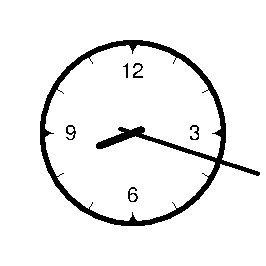
\includegraphics[page=1]{clocks}}
  \qquad
  \subfloat[Med marginal.][\label{fig:times:early}Kiosken stänger snart, men inte nu — perfekt!]{\includegraphics[page=2]{clocks}}
  \\
  \subfloat[I grevens tid.][\label{fig:times:on-time}Precis i tid — du får in ett finger i luckan just när kiosken ska stänga.  Han som jobbar blir sur, och det blir smolk i bägaren.]{\includegraphics[page=3]{clocks}}
  \qquad
  \subfloat[Försent.][\label{fig:times:late}Du är sen — kiosken är stängd.]{\includegraphics[page=4]{clocks}}
  \caption{\label{fig:times}%
    Illustration av \emph{subfloats}.  Den så kallade \emph{bounding box}en visas i \protect\subref{fig:times:late}.  Lägg märke till att bounding boxen har satts så att alla bilder har samma storlek, med enhetlig placering av själva innehållet i förhållande till bounding boxen.  Antag att du ska träffa en kompis för att äta glass just när kiosken stänger för dagen vid 08:30.  När dyker du upp?}
\end{figure}

\section{The YoungDrive App: Iteration 1-4}\label{developed-application}

  After three months time, the app developed has been successful in addressing YoungDrive's goals with the app, with very high precision to the needs and context of the end users. In figure~\ref{fig:iteration-map} the app development from iteration 1-4 are shown. The final app works on web or as an app, online or offline, on all of YoungDrive's Android and iOS devices. The app is fast to use, the back button on the phone can be used to go to the previous view, and the font size and images are consistent for each screen (which was not the case iteration 1-3, see figure \ref{fig:iteration-map} E-3. The goal was to provide a great learning experience, with a strong YoungDrive feel (embracing the values of fun, plus using the YoungDrive logo and colors).

  \todo{Flytta bild till helsida!}
  \begin{figure}[h]
    \centering
    \includegraphics[width=1.0\textwidth]{IterationMapLowRes.png}
    \caption{The app flow described as a timeline (A-I), per iteration (1-4). E.g. in iteration 4, login (B4) appears after choosing quiz to take (A4).}
    \label{fig:iteration-map}
  \end{figure}

  %\subsection{Iteration \#1}

  There was no developed application at this point.

  Instead, two workshops were held, which together would inform the future development of an application.

  There were the findings from those two workshops:

  \subsubsection{Workshop \#1: Customer Journey Map: A day as a coach}

  \subsubsection{Workshop \#2: Quizical and Duolingo}



  The quiz flow during iteration 1-2 was a standard multiple-choice quiz game, designed for assessment, but not for learning. In a scoreboard, they could see which questions they were awarded points for and not, with a total score, see figure \ref{fig:iteration-map} H-1. In the end of iteration 2, whey were encouraged to go back to the start screen, to redo the same quiz again, or select a new one. 1 point is awarded for correct answers, whereas 0 points is given for incorrect answers.

  In iteration 3, feedback for self-reflection was introduced. The coach answers Yes or No on "Are you sure?" for each question (figure \ref{fig:iteration-map} C-3), with the aim of increasing meta-cognitive skills, and being able to give personalized feedback in the score board.

  Thanks to recording both if they were correct and confident, the app can give very precise learning feedback (e.g. showing that the coach answered alternative B with confidence, but showing that A was actually the correct alternative).

  In iteration 3-4, after observing their incorrect answers, and learning their correct ones (closely compare figure \ref{fig:iteration-map} D-3 and E-3), they could retake the wrong answers immediately.

  In iteration 3, the score board was simply showing each correct question with the answer the coach provided versus the correct one. After giving feedback, the coach can train, and improve on incorrect answers and guesses, and when being 100\% correct and confident, ideally take the whole quiz without faults.

  For iteration 4, the score board is more personal, encouraging the coach to reflect on her own learning process. The feedback is designed to give a self-confidence boost ("You were correct, and you were sure" or "You guessed, but you were correct. You can answer with confidence the next time"), unlearn knowledge ("You were incorrect, but you were sure"), or encourage studying more when unsure and wrong ("You were incorrect, and you were not sure").

  To discourage guessing during training, since iteration 3, the coach is shown number of tries on the quiz if they do not get 100\% in their first try (see the top bar of figure \ref{fig:iteration-map} E-3). For iteration 4, the coach will also get a minus point (-1) for answering incorrectly but confidently "Are you sure?": "Yes". If uncertain, the coach should answer "Are yo sure?": "No", and no penalty will be given. The coach will later recieve feedback, either "You can be confident next time" (if correct but unsure) or "How can you get these correct next time?" (if unsure and incorrect).

  The coach is encouraged to be well-prepared before trying again (either consulting the answers or the manuals). At 100\% correct answers, they can get certified, by getting the whole quiz correct without faults. Failing a question on the certification would show that they have not \textit{reliably} learned all the answers during the training. The more effort the coach has put into the training, the more likely the coach will be to pass the certification.

  %Lena Tibell menade vid förslaget att "Belöna inte hur snabbt %en elev går från att kunna till att inte kunna, för olika %människor lär sig olika snabbt". "Vad vi ville åstadkomma %med Antal försök var endast att undvika gissningarna".

   This certification quiz is the same as in training, but no longer do they need to answer "Are you sure?". If the coach can again get 100\% correct answers, without any faults, they have proved they are correct and confident with the topic they should teach the youth.

   If they fail a question, the score board will encourage more training and that they did not get certified, see figure \ref{fig:iteration-map} H-4. Since the coach did get 100\% correct in the training (maybe after a couple of tries) but not in the certification, the knowledge can be described as "Can do with effort". The coach can choose to take a new quiz, or take the same quiz from the beginning of the training.

   For passing the certification on the 1st, 2nd or 3rd time the coach is awarded a Gold, Silver or Bronze medal respectively (after certificate try 3, no medal is given, only the certificate). Compare figure \ref{fig:iteration-map} I-3 to I-4: for iteration 4, the "certificate" mentions the persons name and the topic certified in, which is a form of gamification in addition to the intrisic motivation of rewarding deliberate practice.


In the following sections, you can read more about what data guided the development of the final app, as well as the results from the final app evaluation.

\section{Iteration 1: Uganda Coach Visit}

Here the results from the qualitative and quantitative data for iteration 1 are shown together with conclusions.

\subsection{Qualitative data}

Below, the most important results from the stakeholder and coach interviews are presented.

\subsubsection{Stakeholder interview findings: Entrepreneurship education considerations}
Through early interviews with YoungDrive staff, it is clear that YoungDrive's entrepreneurship education methodology goes hand in hand with the presented theory. It's mottos are: "Dream big, start small", "Learning by doing" and "We have fun!" \citep{youngdrive-manual}.

Both in regards to designing for the users and for the above reason, the app should be a complement to YoundDrive's existing training material and the structure of the program.

A challenging part of the work is that YoungDrive consists of both the practical skills of the entrepreneur, theoretical material of running a business, and an entrepreneurial mindset. Therefore, both how to assess knowledge, and build habits, needs to be examined.

As the stakeholder interviews answered "What's it like being a coach?", their perspectives could now be understood and summed into a early understanding of the coach situation. The stakeholder interviews heavily informed the Questionnaire guide, highlighting aspects that had previously not been taken into account.

\subsubsection{Coach interview findings: Teaching with confidence}

The purpose of the coach interviews was to understand "What's it like being a coach?", from the coaches own perspective. Thanks to having similar interviews with stakeholders, their views could be compared. Also, more detailed answers on background, desires, experience and situation could be provided.

 From the interviews it was understood that CBTs can be responsible for from 7 up to 12 different youth groups in different programs, and such a high number places huge demands on the CBT. Even if there are only 7 groups, being behind on schedule or not being confident, can be very demanding.

%\textbf{Stayover at Patrick:} På morgonen visade Patrick mig hur han jobbar med deras tomt, var det odlas ris, och andra råvaror, deras djur, deras story från Syd-Sudan, till Kampala, till hyddan här i Tororo, och hans värderingar.

%Efter en ungdomssession nästföljande dag besökte vi och hälsade kort på en av de 2 CBT:s vi har session med idag. Sedan hade jag och Patrick den obligatoriska review av ungdoms-sessionen, och jag bjöd honom på middag. Kl. 19 ringde hans fru (som har börjat få tecken av malaria) och skyndade hem.

%Nästa ungdomssession fick jag besöka en annan CBT. Vi var tidiga. Sedan började jag prata med henne, och fick bra tillfälle att intervjua henne och även förklara för henne vad jag gjorde där. Det blev underligt att förklara för henne: Patrick påminde, när jag tabbat mig, att “Marcus, du måste förklara för X vad en app är”. Så hon fick låna min mobil, och jag förklarade att app var kort för applikation, och att för varje applikation har ett eget syfte, t.ex. ta foton. Jag bad henne klicka, svårt, råkade klicka åt henne, men sedan lät jag henne göra. Efter hon sett att det hon såg i skärmen var det hon såg på riktigt, blev hon jätteglad och började fundera vad hon skulle fota. Hon reste sig och gick runt hörnet, och jag följde efter. Hon fotade, efter att noggrannt tänkt igenom, att hon fotade buskarna med frukt. Sedan sade jag hon kunde fortsätta fota, och då tog hon ett litet runt hus utanför.

The interviews with CBTs, Project Leaders and stakeholders led to the realization that different coaches handles this differently well. All coaches possess high self-confidence in varying degrees in various situations, and as a result, quality among coaches is unbalanced, which they see as a challenge. Depending on the situation, everything is going according to plan, you are not confident, or you are falling behind with the schedule, you can be in one of these three Need groups:

\begin{itemize}
  \item The ideal coach
  \item The realistic coach
  \item The challenged coach
\end{itemize}

It was discovered that coach confidence comes largely from being able to have good youth sessions. This is important, because according to the interviews, being a high-quality YoungDrive coach to a large extent means having high-quality youth sessions. For having a high-quality youth session, these are the most important attributes:

\begin{itemize}
  \item Correct information
  \item Correct structure
  \item Time management
  \item Fun atmosphere
\end{itemize}

These findings were used to inform the Customer Journey Map workshop. In addition to the findings here, questions were also asked around etnography.


\subsection{Co-Creation Workshops}

    %What the data said

    Two workshops were held, which together would inform future development of an application. These were the findings from those two workshops:

    \subsubsection{Customer Journey Map: "A Day As a Coach"}

    %After the 15 minute introduction, they started with 5 minutes + 10 minutes discussion mapping out Before, During, After for the ideal coach, John. Green postits were used.

    %Since it took too much time to do this for the other two personas, they were given 5 minutes to either use pink post-its for steps that a realistic coach would skip, and yellow notes that the coach would do differently. This worked well, and the results were discussed within the 5 minutes between the coaches, and explained during 5 minutes witth audio recording.

    %Since they were understandingly tired, they were given a 10 minute break, during which time they were asked to think about things that could go wrong for the sad/angry persona, Suzan. When I got back from the toilet, they had already started working! I took time of 5 minutes, and they walked through the concerns and it’s effects, just like they had did with the 2nd persona.

    The three coaches understood the concept of the workshop surprisingly effortlessly, although the concept of postits and Customer Journey Map and Personas were unfamiliar to them. Contributing to the energy, was probably that the timeline and personas were largely informed by their interview answers. The workshop gave great insights for understanding the coach situation and the coaches themselves, both observing their behaviour during the workshop and learning about all the unknown activities involved in being a coach.

    The first workshop was concluded with many important insights. Thanks to using Personas, it was discovered from the workshop that the difference between coaches and the quality of the youth training was more diverse than originally thought. This is especially true when the coaches prepares for their youth session, an activity which was regarded as important as the coach training, but where quality of preparations were very divergent. This could be a great opportunity for delivering the app's promise of distance learning (see section \ref{purpose}). The teacher Josefina in an after-interview commented that while she can influence the coach training by her physical presence, she currently has no influence or insight into how the coach prepares, more than the co-project leaders' reports. When preparing for a session, there is a wide variety of \textit{when} the planning happens, and how a coach judges what amount of preparation is enough.

    Most coaches plan their next session during the morning, or immediately after a session with their group. Since a coach has somewhere between 7-10 groups (some even more), and the youth groups are at different modules, there is a lot of knowledge for the coach to handle - not only theoretical knowledge, but also the struggles of the youth, assignment presentations, workshops to be facilitated, etcetera. It is easy for a coach not to do everything as planned or as specified in the manual. Most of the coaches are said to be motivated by the possibility of becoming a better coach.

    According to the workshop, most of the coaches assess if they were ready for a topic \textit{after} a youth session. The feedback from the youth, as well as their questions and how well the coach can answer these, are the biggest informant. The exception is if the local project leaders comes to visit the youth session, but they do seldom have time to visit all of the coaches during a month, and during a month coaches should have taught 4 topics to all of their groups.

    \subsubsection{Smartphone Test using Quizoid and Duolingo}

    Quizoid (see figure \ref{fig:quizoid}) and Duolingo (see figure \ref{fig:duolingo}) were tested to understand the technical possibilities of the coaches, see figure \ref{fig:smartphoneTest}. They had circa 45 minutes to spend in each app, with discussions after each app test. The result was that the app can place itself somewhere in the middle of the two, regarding difficulty level.

    \begin{figure}[h]
        \centering
        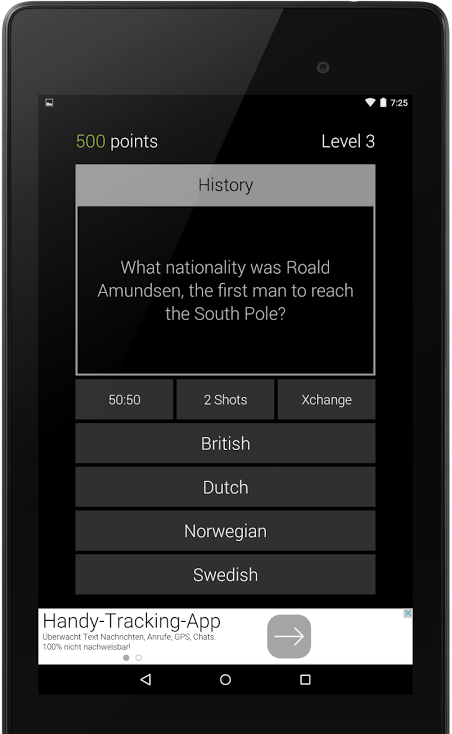
\includegraphics[width=0.5\textwidth]{quizoid.png}
        \caption{Quizoid is a simple multiple-choice game \citep{quizoid}, tested by coaches in iteration 1}.
        \label{fig:quizoid}
    \end{figure}

    \begin{figure}[h]
        \centering
        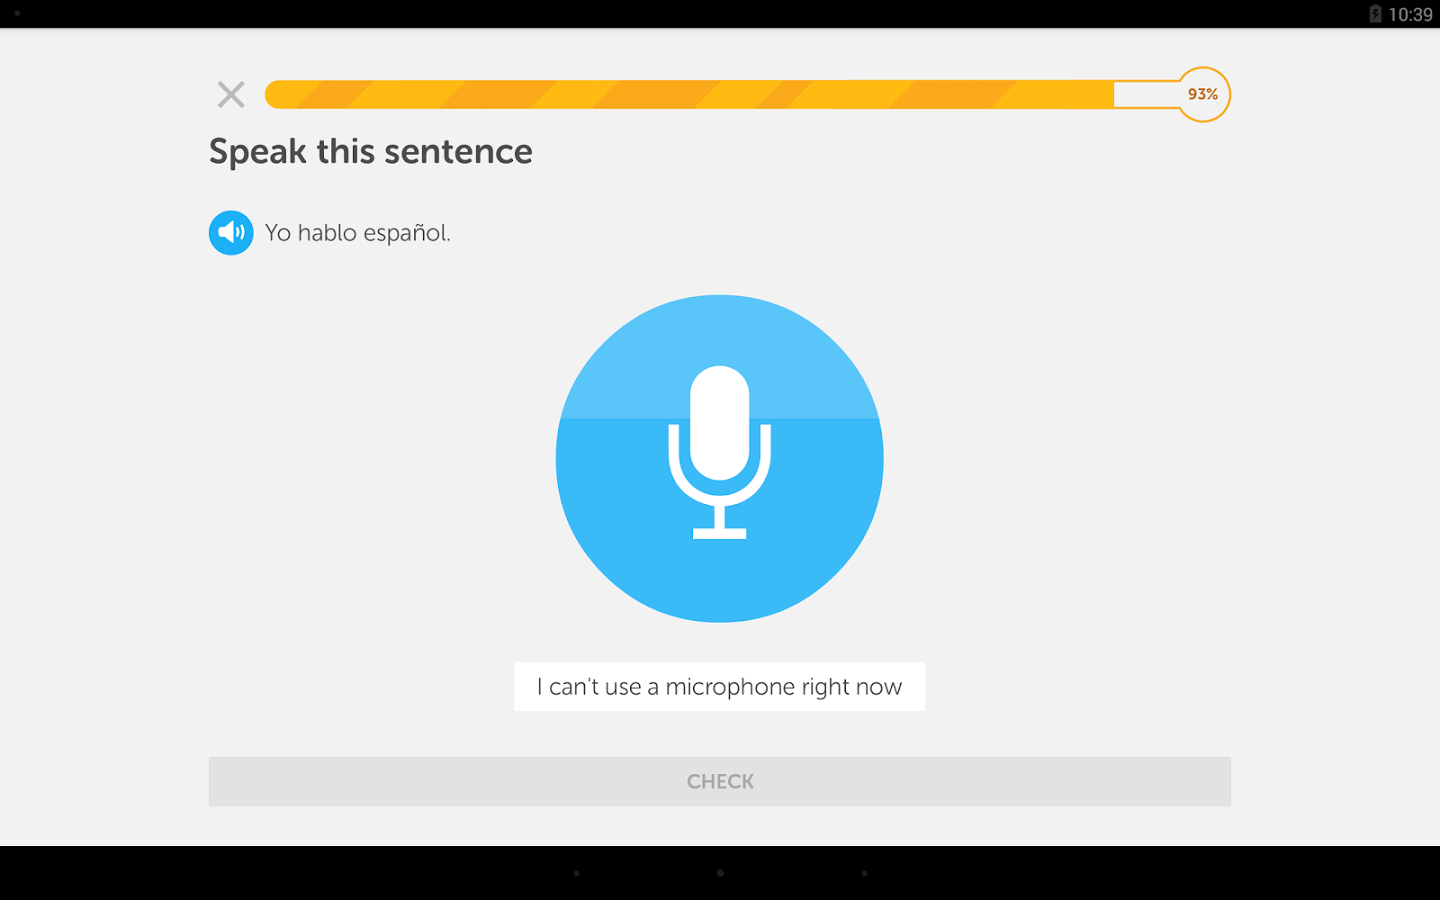
\includegraphics[width=0.7\textwidth]{duolingo.png}
        \caption{Duolingo is a praised app for language learning \citep{duolingo}, tested by coaches in iteration 1}.
        \label{fig:duolingo}
    \end{figure}

    \begin{figure}[h]
        \centering
        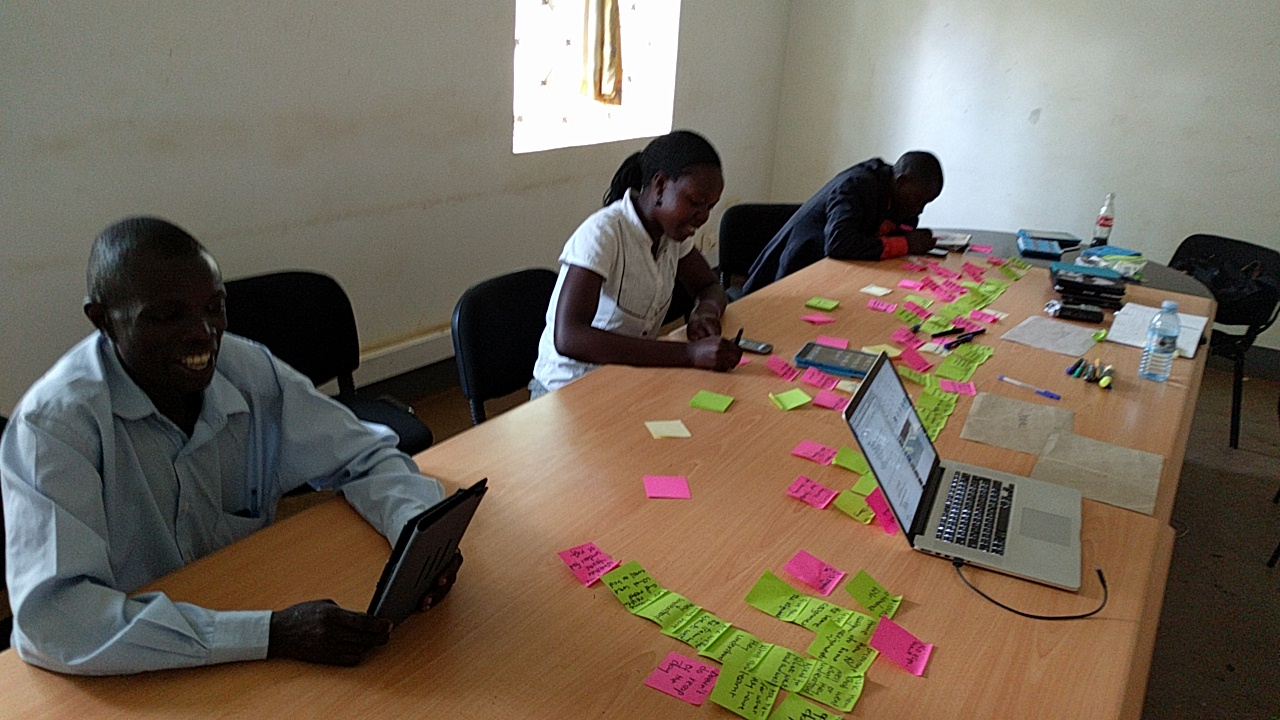
\includegraphics[width=0.7\textwidth]{iteration1/smartphoneTest.jpg}
        \caption{Picture from the smartphone test, observing how the coaches comprehend using Duolingo and Quizoid for the first time.}
        \label{fig:smartphoneTest}
    \end{figure}

    \clearpage

    Two of the three YoungDrive coaches (two of them being the local project leaders) used a smartphone for the first time. The attitude towards using a smartphone was overwhelmingly positive. One of the coaches even mentioned: "Marcus, today one of my dreams have gone true" regarding using a smartphone for the first time. He even asked if he could borrow one of the devices during the remainder of the stay. Even for coaches that had never touched a smartphone before, some concepts were easily understood (like using the camera and Quizoid).

    Other concepts were harder (accidently getting to the settings menu, unlocking the device, understanding advanced games, or training languages using Duolingo with advanced interactions). Point and click is easily understood, whereas sliding is much more unnatural.

\subsection{Discussion}

During a evaluation meeting with Linköping University and YoungDrive, it was determined that Iteration \#1 did provided answers for research question \#1, \#2, and \#3, and partly \#5. Thus, the iteration could be considered very successful, and now, the development of the app could begin.

It is clear from the data that the motivation of the app should be to assess and strengthen the entrepreneurship knowledge and skills of the coach. For coach quality to improve was a desire from the stakeholders as well as the coaches themselves, even if they were also satisfied with the current results. This lead to a challenging situation how an app can address becoming a better-performing coach.

An app could increase accuracy of correct information. With an app, the coach could keep a record of the module content, and see when and if they do need to refresh their skills. It was discovered that a coach app can benefit not only the coach training, but also in a surprisingly precise way, what was called "distance learning" in section \ref{purpose}. Accountability if the coach is ready for a session by automatic assessment. A very important aspect to increase learning and confidence will be to give good feedback (see section \ref{learning-assessment}).

With all the possible benefits of an app, it is definitely a problem that so few coaches have smartphones. Either continued development could be guided solely by the use case of having an app tailored for the coach training (where donated devices are available). But this would be to ignore that an app helping the coach to prepare for a session would be extremely beneficial, which discovered during the field visits to youth sessions and during interviews.

The motivation for using technology is very high, so one way forward would be that the app for distance training will reach only the users that can be given access to a smartphone, counting that more coaches will get smartphones in the future. Not using smartphones but feature phones (which all coaches possess), would mean building an SMS-based service (see \ref{rq1}.

As most coaches are already motivated to become a better coach and using technology, Sierra's \citep{sierra} advise of designing for their compelling context can be followed. From a YoungDrive perspective, this might mean "Given a teaching situation among the youth group, a great coach can teach an entrepreneurship topic more consistent with what the coach material said". Their performance in the YoungDrive app could translate into: "Given a question in the app, a great coach will get the right answer more often, and increasingly leverage the correct answer to their coach situation".

\subsection{Next iteration}
It is agreed with Josefina that the most important found skill of a YoungDrive coach is having great youth sessions. It is a challenge that the coach surely needs to feel, but does not always possess, self-confidence for its youth session. This partly stems from the lack of practical experience being put into realistic situations during the coach training.

If self-confidence comes from being able to deliver Correct Information, Correct Structure, Time Management and Fun Atmosphere, an app strengthening these will surely improve youth session quality. According to Josefina, assessing and increasing Correct Information is the parameter she values the most highly, and this will be the continued primary focus of the master thesis.

It is agreed with Josefina that preparing for a youth session can have an increased focus. It is a worry that designing for both the coach training and preparing for a session might be too ambitious within the given time frame. If so, designing for the coach training is deemed more important.


\section{Iteration 2: Zambia Coach Training}

Here the results from the qualitative and quantitative data for iteration 2 are shown together with conclusions.

\subsection{Qualitative data}

\subsubsection{Design workshop \#1 in Zambia}

The result was fantastic, in the sense that it gave me an unbiased look at what the coaches expected from the app, what functionality wasn't important, and into their technical preferences.

The designs and insights gained were used throughout the week to further improve the app I had actually started creating, and gave great insights to who the coaches were and their thinking. \todo{Add image here}

\subsubsection{The desire perspective}

Insight: "The app could be used on my spare time". This is particularly true, about the bonus quizzes that were produced during the week.

Insight: \textit{Coach:} "I'll buy one" (a smartphone), \textit{Response from other coaches: } "Whoa!"

\subsubsection{The utility perspective}

Ideation: "The app should have notes, not only quesitions"

\subsubsection{The usability perspective}

Low resolution screens, made the text be barely visible. This showed, that the app needed to be tested on a lot of different devices. This is particularly true, as on day 1, the coaches did not know how to zoom, which could cause accident refreshs, frustration or confusion.

The app needs to work offline! To be online on the phone is too expensive for the coaches, and too unrealiable to give a satisfactory experience. Also, during testing, relying on internet can cause a lot of problems, especially if the teacher is alone.

\subsubsection{The learning perspective}

    The coaches had surprisingly high results, and at day 3 they wished harder questions when asked.

    We responded by having harder questions, e.g. by introducing similar answers, and testing 4 alternatives instead of 3. This was appreciated.

    The following analysis could be done:

    \subsubsection{Doing a pre-quiz: good for learning}
    When asked about what they thought about doing "Graduation" as a pre-quiz (before the session), 10/10 said they liked doing the quiz before, and that it benefited their learning during the session.

    When asked why it helped, these were the results:

    \begin{itemize}
    \item "During session, it is easier to follow" - 10 (100\%)
    \item "Giving the paper manuals before, scanning headings and pictures etc, would not help" - 10 (100\%)
    \end{itemize}

    It was also tested to work in group or individually. The ones who answered, said that you learned more individually (3/3), and more fun doing it together (3/3). Doing it together, was enjoyable as it was "Very easy because of using different minds" and "We can collaborate to do better".

    \subsubsection{Doing a post-quiz: Spaced versus massed learning}
    In "Goal setting", quotes were "I thought it was fun and challenging to do the quiz immediately afterwards", with another coach commenting "The mind was still fresh".

    When asked on timing preference, 10/10 said it would be more fun to do the quiz immediately afterwards, not at the end of the day. The motivation, seemed to be that it was easier.

    9/10, said they wanted to do the quiz afterwards. The outlier, said it would be better for learning doing it later.

    After this comment, this was the distribution:

    \begin{itemize}
    \item 3/10 wants to do the quiz both before and after a session
    \item 1/10 wants to do the quiz before and at the end of the day
    \item 7/10 wants to do the quiz only immediately afterwards
    \item 10/10 wants to do the quiz immediately afterwards, and then again at the end of the day
    \item 7/10 wants to do the quiz immediately afterwards, and then a joined quiz with other topics at the end of the day
    \end{itemize}

\subsubsection{The teacher perspective}

  \textbf{Low scores}
  The 9/19 shows the relevancy of the quiz, as Josefina did not think she would have discovered that the coach was lagging behind otherwise.

  In the data, it was observable that the coach had done well together with others, but 3/7 when done individually.

  Josefina said about the 9/19: "This is where a control group would be beneficial". "He is often passive during open questions, but active during the team exercises."

  The question we needed to ask ourselves, was: "Does this imply he is a good or bad coach?".

  \textbf{What would hinder Josefina from using the app}

  Josefina says: "Not doing data collection digitally works whenever they are 10 - but not with bigger numbers than that."

  According to the final interview with Josefina, she does not wish the app to replace her. She enjoys teaching, thinks she has an important role, and suggests the app to be designed to support her and the coaches, not replace her.

  \textbf{Acceptance criteria}

  If you have a high score, you are ready. If not, you need to redo the quiz.

  If you are 8/10 or lower, you are in the red zone. If lower than 10/10, they are not ready, the motivation being that what they don't know, they will teach in an improper way: affecting hundreds of youth. This is why Josefina thinks they should need all of the answers correct.

  \textbf{Testing Correct Structure, Time Management and Fun Atmosphere}
  Josefina informs that Correct Structure, Time Management and Fun Atmosphere would be the most valuable to test after a youth session. She also notes, that \textit{some} aseessment could be made via the app before a session. Because of the reason that this thesis does not focus on after-session-evaluation, Correct Information is primary to improving on the other factors, which are secondary.

\subsubsection{The developer perspective}

  \begin{itemize}
    \item Bugs was a big hindrance to functionality, and a lot (both high-dose, and high-scale) of testing is very important
    \item Simpler design than I thought (KISS) was sufficient
  \end{itemize}

\subsubsection{Bonus results: Testing the app on Kampala university student}
The app was tested on a university student from Makarere University.

The university student from Makarere University scored 100\% correct, in spite of not having any entrepreneurship training. This showed that guessing was possible, or that the quizzes were too easy.

\subsection{Quantitative Data}

    %What the data said

    This section presents the results from the two workshops held, in form of lessons learned. Also, some of the quiz results are shown.

    \subsubsection{Quiz Results from the Coaches}

    Quiz results ranges from the worst on 24\% (getting 4/17 correct answers) to 100\% (which has happened on 52/101 instances, for all of the quizzes). Week 9 was undoubtably the hardest quiz, with the topic being "Goal Setting and Action Plan" (17 questions, average being 76.22\% correct answers, 18 quiz results submitted). The easiest quizzes are week 3 "Financial literacy" (11 questions), week 6 "Mastering sales" (9 questions) and week 7 "Sales day" (3 questions), where all of the results are 100\%.

    There are some amount of coaches that have taken the same quizzes multiple times. From this, interesting conclusions can be drawn. Attending the lecture shows a 15.0\% average increase in quiz results, compared to an 12.8\% increase with simply taking the quiz two times. This shows that a lecture is still more effective than learning via the app.

    Time to finish a quiz took between 2 minutes to 33 minutes (3/4 quizzes that took longer than 25 minutes were on quiz 9, there is a correlation with number of questions). Most of the quizzes took under 5 minutes to complete, and results are always over 80\% for these instances. This shows that the coach had a high confidence with the answers. Similarly, all of the scores under 60\% has taken more than 20 minutes. This can be explained by that the coach is unfamiliar with the app or smartphone, and that the coach is uncertain of the answers.

    It is seen in the quiz results that the quizzes did get gradually more challenging, as the average of quiz scores gets lower after day 3 of training, when it was discovered was welcoming the quizzes to get harder.

    The quiz scores when quizzes are performed in group is very varying (from 24\% to 100\%), and it is observed that influence of another coach can lead both to a worse score than their individual average, and a higher score. It is interesting to see that the three coaches that have the worst average (67, 72 and 85\%) are also the ones that have taken quizzes the least times individually, and the most taking quizzes together with others. This may show that the app is more effective when used individually, and there seem no other connection to previous entrepreneurial activity or background.

    There are few correlations that can be made between the coach's background and experience, compared with quiz results or app behavior. Nothing in the coach information distinguishes the worst 3 performers in the quiz. For the opposite, there is however a noticable behaviour that being confident, having trained youth, leadership experience, business experience, care for community, care for oneself and confidence to take on many youth, almost guarantees a high quiz average (which demonstrates learning) and quizzes done (which demonstrates motivation).

    For coaches with 0-1 negative remarks during the interviews (n=6) compared to coaches with 2-4 negative remarks (n=4), their quiz average is but 2\% higher (87\% to 85\%). This is not significant, but this number is increased to 93\% (an 8\% increase) if the outlier from the group is removed (a coach which only did three quizzes with average of 57\%). In the future, more research could be done into comparing coach data with quiz results.

    %Comparing instances when coaches have taken a test before and after a lecture, the results are: 71\%to 100\%, 59\% to 74\%, 80\% to 86\%, 90\% to 100\%. Without the lecture, improvements has been from 80 to 90, 100 to 100 to 100, 90 to 90, 80 to 100, 90 to 100, 100 to 100, 86 to 100, 100 to 100, 90 to 100.

    \subsubsection{Lessons Learned from Unbiased App Design by Coaches: Use Case 1}

    The result was fantastic, in the sense that it gave an unbiased look at what the coaches expected from the app, what functionality wasn't important, and into their technical preferences. A simpler design than originally thought was deemed sufficient, and the simple sketches guided continued development of the app during the week. From using the devices, it was found that most coaches prefer using the tablet (5 for tablet, versus 2 for smartphone and 2 for computer). Both the designs and insights gained were used throughout the week to further improve the simple app created at the end of iteration 1. The workshop gave great insights to who the coaches were and their thinking. \todo{Add image here}

    \subsubsection{Lessons Learned from Unbiased App Design by Coaches: Use Case 2}

    During this workshop, the focus was to examine what builds confidence among the coaches. The following clusters could be determined: "I believe in myself" (3 coaches), "I believe in God" (2 coaches), "I am well prepared" (4 coaches) and "I am certified" (1 coach). See figure \ref{fig:zambiaWorkshop2} for the different clusters.

    \todo{Make full-page}
    \begin{figure}[h]
        \centering
        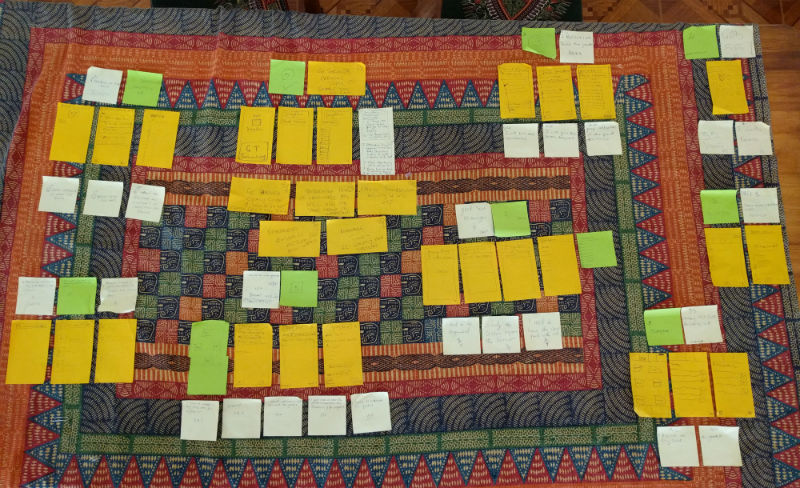
\includegraphics[width=0.7\textwidth]{zambiaWorkshop2small.jpg}
        \caption{The clustered postits with needs, together with included design proposals.}
        \label{fig:iteration}
    \end{figure}

    Josefina comments after the workshop: “I have a problem: There is no way I can control them how they have prepared themselves for a youth session.", says Josefina.

\subsection{Analysis of Questions in Regards to Bloom's Revised Taxonomy}

%Analysing the quiz questions is one of the most important prerequisites to evaluate the learning effect of the app.

%The analysis of the questions showed that in general, where the question performed on Bloom's Revised Taxonomy got gradually higher for each new topic.

Analysing the questions by each topic according to Bloom's Revised Taxonomy, showed that questions on average gradually reached higher levels on both the knowledge dimension and the cognitive dimension. In topic 1 of 10, most questions only reached the first level of the knowledge dimension ("Factual") and cognitive process dimension ("Remember"). In quizzes created at the end of the week (like topic 9 of 10), questions reached up to "Analyse" on the cognitive process dimension (level 4, not reaching "Evaluate" or "Create"), and the whole range of the knowledge dimensions ("Factual, "Conceptual", "Procedural" and "Metacognitive").

\subsection{Discussion}

The quantative and qualitative data from iteration 2 shows that the app works for "validating the coaches' level of knowledge during their education", which was the main purpose of the master thesis (see section \ref{rq}. Now, the app should be tested in Uganda as well, and there can be an increased focus on "distance training" and "certify all staff".

Iteration 2 has translated the theoretical understanding of answering research question 1, 2, 3 and 5 into practical experience. Now there are observable evidence for what the interactions from Iteration 1 showed:

\begin{itemize}
\item The purpose of the coach training should be to prepare the coach in having great youth sessions
\item Therefore, this is what the quizzess should assess
\item What it really means being a good YoungDrive coach, is having good youth sessions
\item
\end{itemize}

\subsubsection{Validating the coaches' level of knowledge}
The quiz results data shows that a lecture is still currently more valuable than taking a quiz in the app two times to improve (15.0\% to 12.8\%). For iteration 2, work on answering research question 4 has started. While the teacher has appreciated the multiple-choice assessment, challenges of designing test questions to support entrepreneurial learning has been found. It is clear that the app is valuable for assessment, increasing coach self-awareness and being a valuable indicator for the teacher. However, the questions formulated scores low on Bloom's revised taxonomy \cite{bloom} compared with YoungDrive's educational objectives for the topics.

There are previously found issues with using multiple-choice for assessment and learning, but they seem to become especially relevant in the context of teaching entrepreneurship.

Either question formulation needs to be improved, or creative design solutions needs to be experimented with which can increase coach understanding and identify and reduce guessing. This needs to be further investigated for iteration 3.

Test with university student scored 100\% correct, means that common sense can go a long way, and that the results can't be 100\% trustworthy, and that multiple-choice questions has serious issues - this, we already knew during and before the coach training - but it needs to be taken care of. Similarly business and leadership experience for the coach seems to lead to a higher quiz average, while a low quiz average can't seem to be relatable to any of the coach characteristics found during the interviews. This makes it hard to design the app for different types of coaches, without testing other parameters, which should be done in iteration 4 for the summative test.

\subsubsection{Distance learning}
In addition to the formative app tests, workshop \# 2 heavily informs what is necessary when designing for use case 2, distance learning: preparing a session in regards to building confidence. The results from the workshop are somewhat surprising, factors not only those that relate to the four parameters from iteration 1 ("I am well prepared" and "I believe in myself"), but for some also "I believe in God" or "I am certified" (which relates to purpose 3 of the app). These should be considered for iteration 3.

Further, app tests expose how the app is currently not actively designed with learning in mind, and thus not distance learning. This is unfortunate, both because distance learning is important, and as the app test with refugee innovators shows that there is an opportunity doing entrepreneurship training in rural areas outside of YoungDrive's coverage area. In order for online coach-training to work for distance learning, learning and feedback, and not only assessment, is however essential.

While it may be technically possible, the teacher desires the app support her during the coach training, not replace her. Therefore, completely replacing the teacher with an app should be avoided. The teacher is very important for giving coaching and educating in a way that the app can't. But the teacher can also be empowered by the app. For the future, Josefina would have liked to be able to stop coaches from having taught, if they do not have 90-100 \% correct information on the subject. Today, Josefina can not assess this. This means that some coaches, are teaching incorrect information to hundreds of youth. Here, the quiz has a very good need to fill.

If wrong on an answer, the app today has no means of giving high pay-off tips to get to 100\%, or exposing you to deliberate practice or perceptual exposure. If the coach gets 9/10 correct answers reliably, or gets 5/10 answers with guesses, the coach still needs to retake all answers, not having learned the correct answer before taking the quiz again.

How to develop the app to solve these issues, is not obvious. Multiple strategies could and should be used. The app could benefit from introducing smart feedback encouraging a growth mindset ("You did not get 100\% \textit{yet}") \cite{dweck}.

\subsection{Next iteration}
After the meeting with the partner and expert group, the following was concluded from iteration \#2:

\begin{itemize}
\item The app is partly working on assessment now, but not for learning. Are coaches really learning via the app, especially learning to be better coaches?
\begin{itemize}
  \item Multiple-choice is flawed in its current form. How can guesses be identified and reduced in a multiple-choice format? How can answering questions improve confidence and encourage learning?
  \item How can questions be formulated in a way that teaches entrepreneurship, which is so practical?
\end{itemize}
\item The need for a field app still feels relevant (especially for sessions long since the coach training)
  \begin{itemize}
  \item An app could be used, either before you start planning (to guide what you need to study the most on), or after you think you are ready (so you can assess and improve).
  \item When designing the app, it is concluded that an app for coach training, and an app to use before a youth session, should be able to be the same app if possible, since the purpose of preparing the coach to be great with its youth session is the same.
  \item Discussing the importance of self-reflection after a youth session with Josefina, led to asking more of such questions in coach quizzes. While Fun Atmosphere can be hard to assess using multiple-choice, can Correct Structure and Time Management be assessed?
  \end{itemize}
\end{itemize}

After the partner and expert meeting, it was decided that the following needs to be done for iteration 3:

\begin{itemize}
  \item Make sure that the coach actually learnes the desired educational objectives
  \begin{itemize}
    \item Create a new quiz guided by Josefina, "Are you ready for Session 9?", also to test if Correct Structure and Time Management could be assessed using multiple-choice
    \item See if design additions to multiple-choice can increase learning in-line with Bloom's revised taxonomy
  \end{itemize}
  \item Design quiz app for learning, focus on field app, and have a design that works stand-alone from the YoungDrive coach training in mind.
  \begin{itemize}
    \item Investigate the effect of giving growth mindset feedback in the app (The Power of Yet approach)
  \end{itemize}
  \item Test if the app created in Zambia could work also in Uganda
    \begin{itemize}
      \item This also means converting all the questions from the new (Zambia) manual to the old (Uganda) manual, since both structure and content of the manuals has changed.
    \end{itemize}

  \end{itemize}
\end{itemize}


\section{Iteration 3: Uganda Formative Test}

Here the results from the qualitative and quantitative data for iteration 3 are shown together with conclusions. For the coach training in iteration 1, designing the app only for assessment but not for improvement was acceptable, since Josefina could give feedback in person. This meant that scoring low (like 5/10) or high (like 9/10) on a quiz after a session, the coach not taking the quiz again was not mandatory. Josefina could observe the results, and complement the missing information in an upcoming lecture or give immediate feedback herself.

In contrast, image the situation of using the app being weeks or months \textit{after} the training, and Josefina is no longer available. Instead, the coach uses the app exclusively one hour before a youth session, to assess if the coach is ready. If a coach receives the score 5/10 or 9/10, what should happen? Clearly, in this case the app should be designed to not leave the coach alone, but help the coach to get smart feedback, encourage the coach to try again and improve their score, and again assess if the coach is fully ready for teaching the youth in the given topic. This new design of the app was the focus of the interactions from iteration 3, the results observable below.

\subsection{Qualitative data}

  %What the observations said

  \subsubsection{Observations from Kampala test}
  The entrepreneurship student in Kampala, informed the following changes:

  Instead of "Become certified", he would be more motivated by unlocking the opportunity to apply the skills.

  "Improve" should be renamed "Try again", because it is more intuitive.

  His overall opinion on the app was:

  "Can you give me the link, because I'd love to do more of this. I think it's amazing."

  \subsubsection{Verified relevancy of seperating Training and Certification}
  When asked for an opinion, Josefina answered: "I like the idea that when the coaches have answered all of the questions correctly, they can consilidate the knowledge by the certification test, when the coach should get 100\% correct on their first try."

  \subsubsection{Field visits}

  The first thought was to use Gold/Silver/Bronze in the Training mode, and "Are you sure?" in the Certification mode. User tests showed that the other way around was better.

  \subsubsection{Big app test}
  \textbf{Learning: } The app test simulated the app being used to assess preparedness for a youth session. They clearly showed evidence between the difference between designing for Assessment and Learning:

  Given a coach having prepared for their youth session on week 9, and then only scoring 5/10, what should happen? In a similar way, what should happen if 9/10 correct answers?

  For the coach training, the assessment was okay, since Josefina could pick up and give feedback.

  Before a youth session, leaving the coach there is not viable. If the coach has 9/10, that coach should not only be let be, and especially if the score has been 5/10.

  Feedback was that one user did not want to press "Improve", until having read the manual. The motivation was: "Not because that is what the info says, but because I can learn more from the manual, about more than what the questions says."

  This is indeed the preferred behaviour from Josefina, and the app should continue to encourage only using the app training or certification mode after having prepared via the manual. This way, the app is still assessment, but it is "learning by thinking", with feedback.

    %What the data said

    \subsection{Big Formative App Test}
  The app test simulated the app being used to assess preparedness for a youth session. The test clearly showed evidence between the difference between designing for Assessment and Learning. See figure \ref{fig:tabletTest} and figure \ref{fig:computerTest} to understand the setting.

  Before the quiz started, the coaches were asked to raise their hand if they felt proficient with using a smart phone. 8 out of 23 said yes. After using the app, 16 thought they were proficient (25\% increase), while 5 said low proficiency, and 2 said no (we don't yet feel proficient, still fear).

  The test was done in pairs, because of lack of devices. Manual data collection of quiz results was not viable with coaches more than 10 people (as Josefina said in Zambia), it got to hectic, which is why not all quiz results were recorded, only when coaches raised their hands, which they often did only when they got 100\%, and some never raised their hand. The results gathered can be seen in figure \ref{fig:iteration3data}.

  A couple of notes can be made from the quantitative data. 6 groups consisted of two CBTs, and 5 groups were mixed (1 CBT and 1 Youth Mentor in the group). Among the CBT groups, the average score on a quiz was 77\%, while the presence of a Youth Mentor increased the average to 98\%. The groups were free to choose whichever quiz they wanted to. Only one group chose to redo the same quiz (scoring 100\% both times), while all others varied between different quizzes. Out of 18 quiz instances, 85\% was the mean (versus a 89\% average over 105 instances in Zambia), with 1 instance of 0\% (0/15!), 35\%, 53\%, 71\%, 2 instances of 83\%, and 12 instances of 100\%. The lower result than in Zambia could be that in Zambia the topics were still fresh, and that in Uganda, much of the information from the earlier topics of the training has not been repeated in a long time.

  \begin{figure}[h]
    \centering
    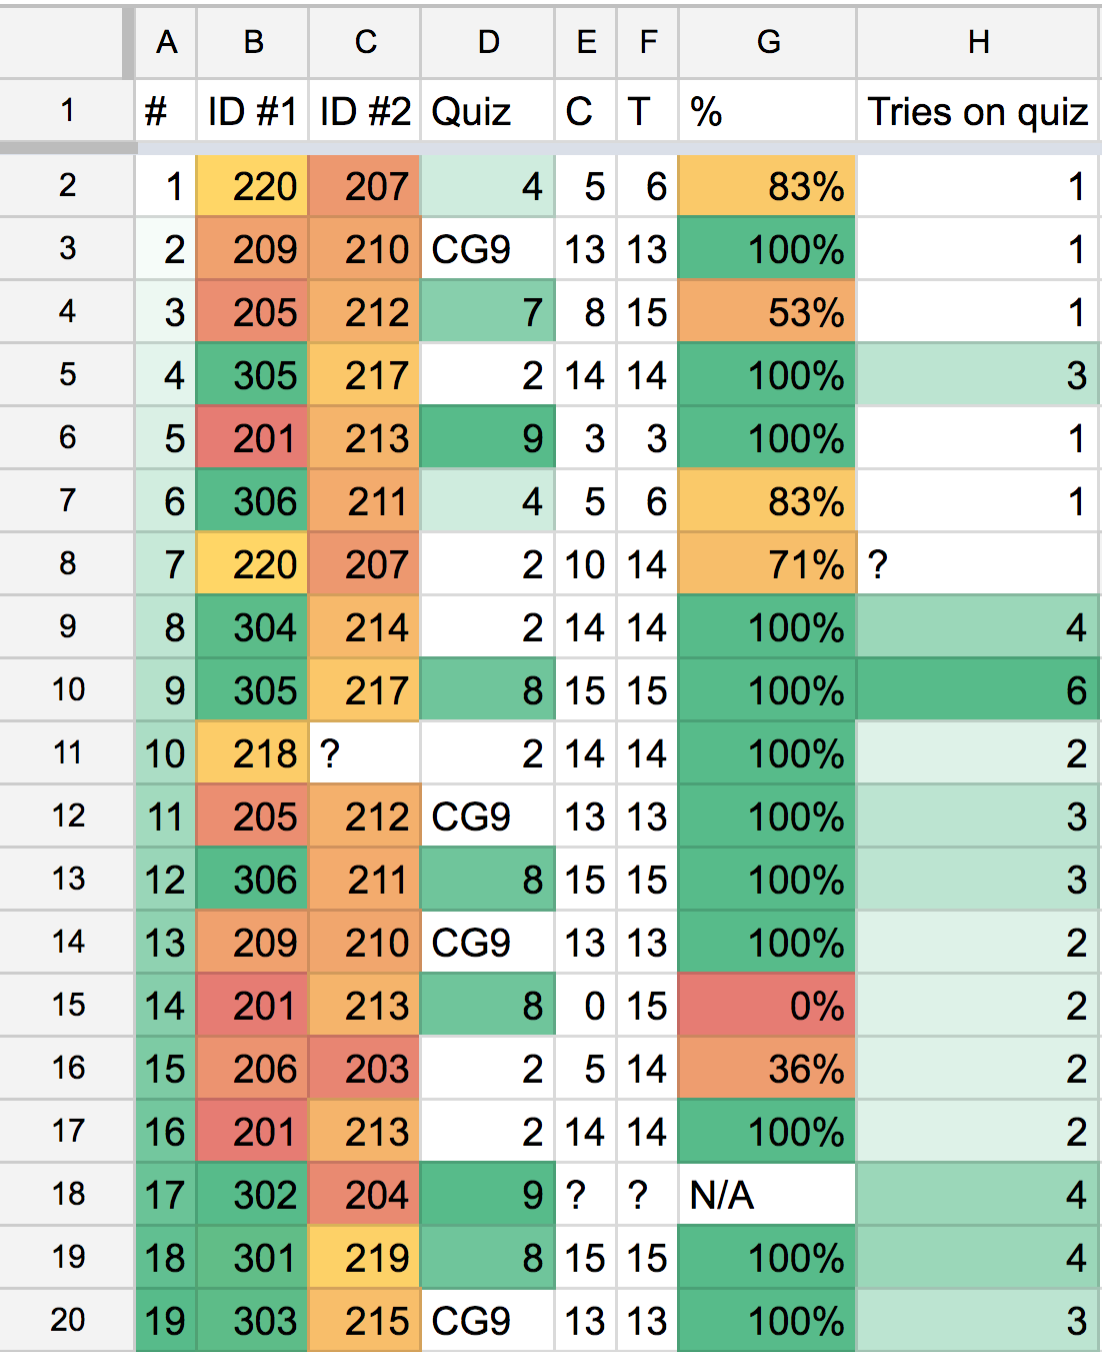
\includegraphics[width=0.8\textwidth]{analysis/iteration3data.png}
    \caption{The data gathered from iteration 3. A is order of quiz submission, B and C is Coach ID for coach 1 and 2 in the group, C is quiz chosen (CS9 meaning "Coach guide week 9"), D is correct answers, E is number of questions, G is percentage correct answers, and F is recorded quiz try on the particular topic at the time of submission.}
    \label{fig:iteration3data}
  \end{figure}

  An aspect which makes the data analysis less usable is that since the quizzes were carried out in pairs, the results are non-traceable to individuals, and pre-knowledge about the coaches or for iteration 4. This is why such a large focus has been on observations.

  \begin{figure}[h]
    \centering
    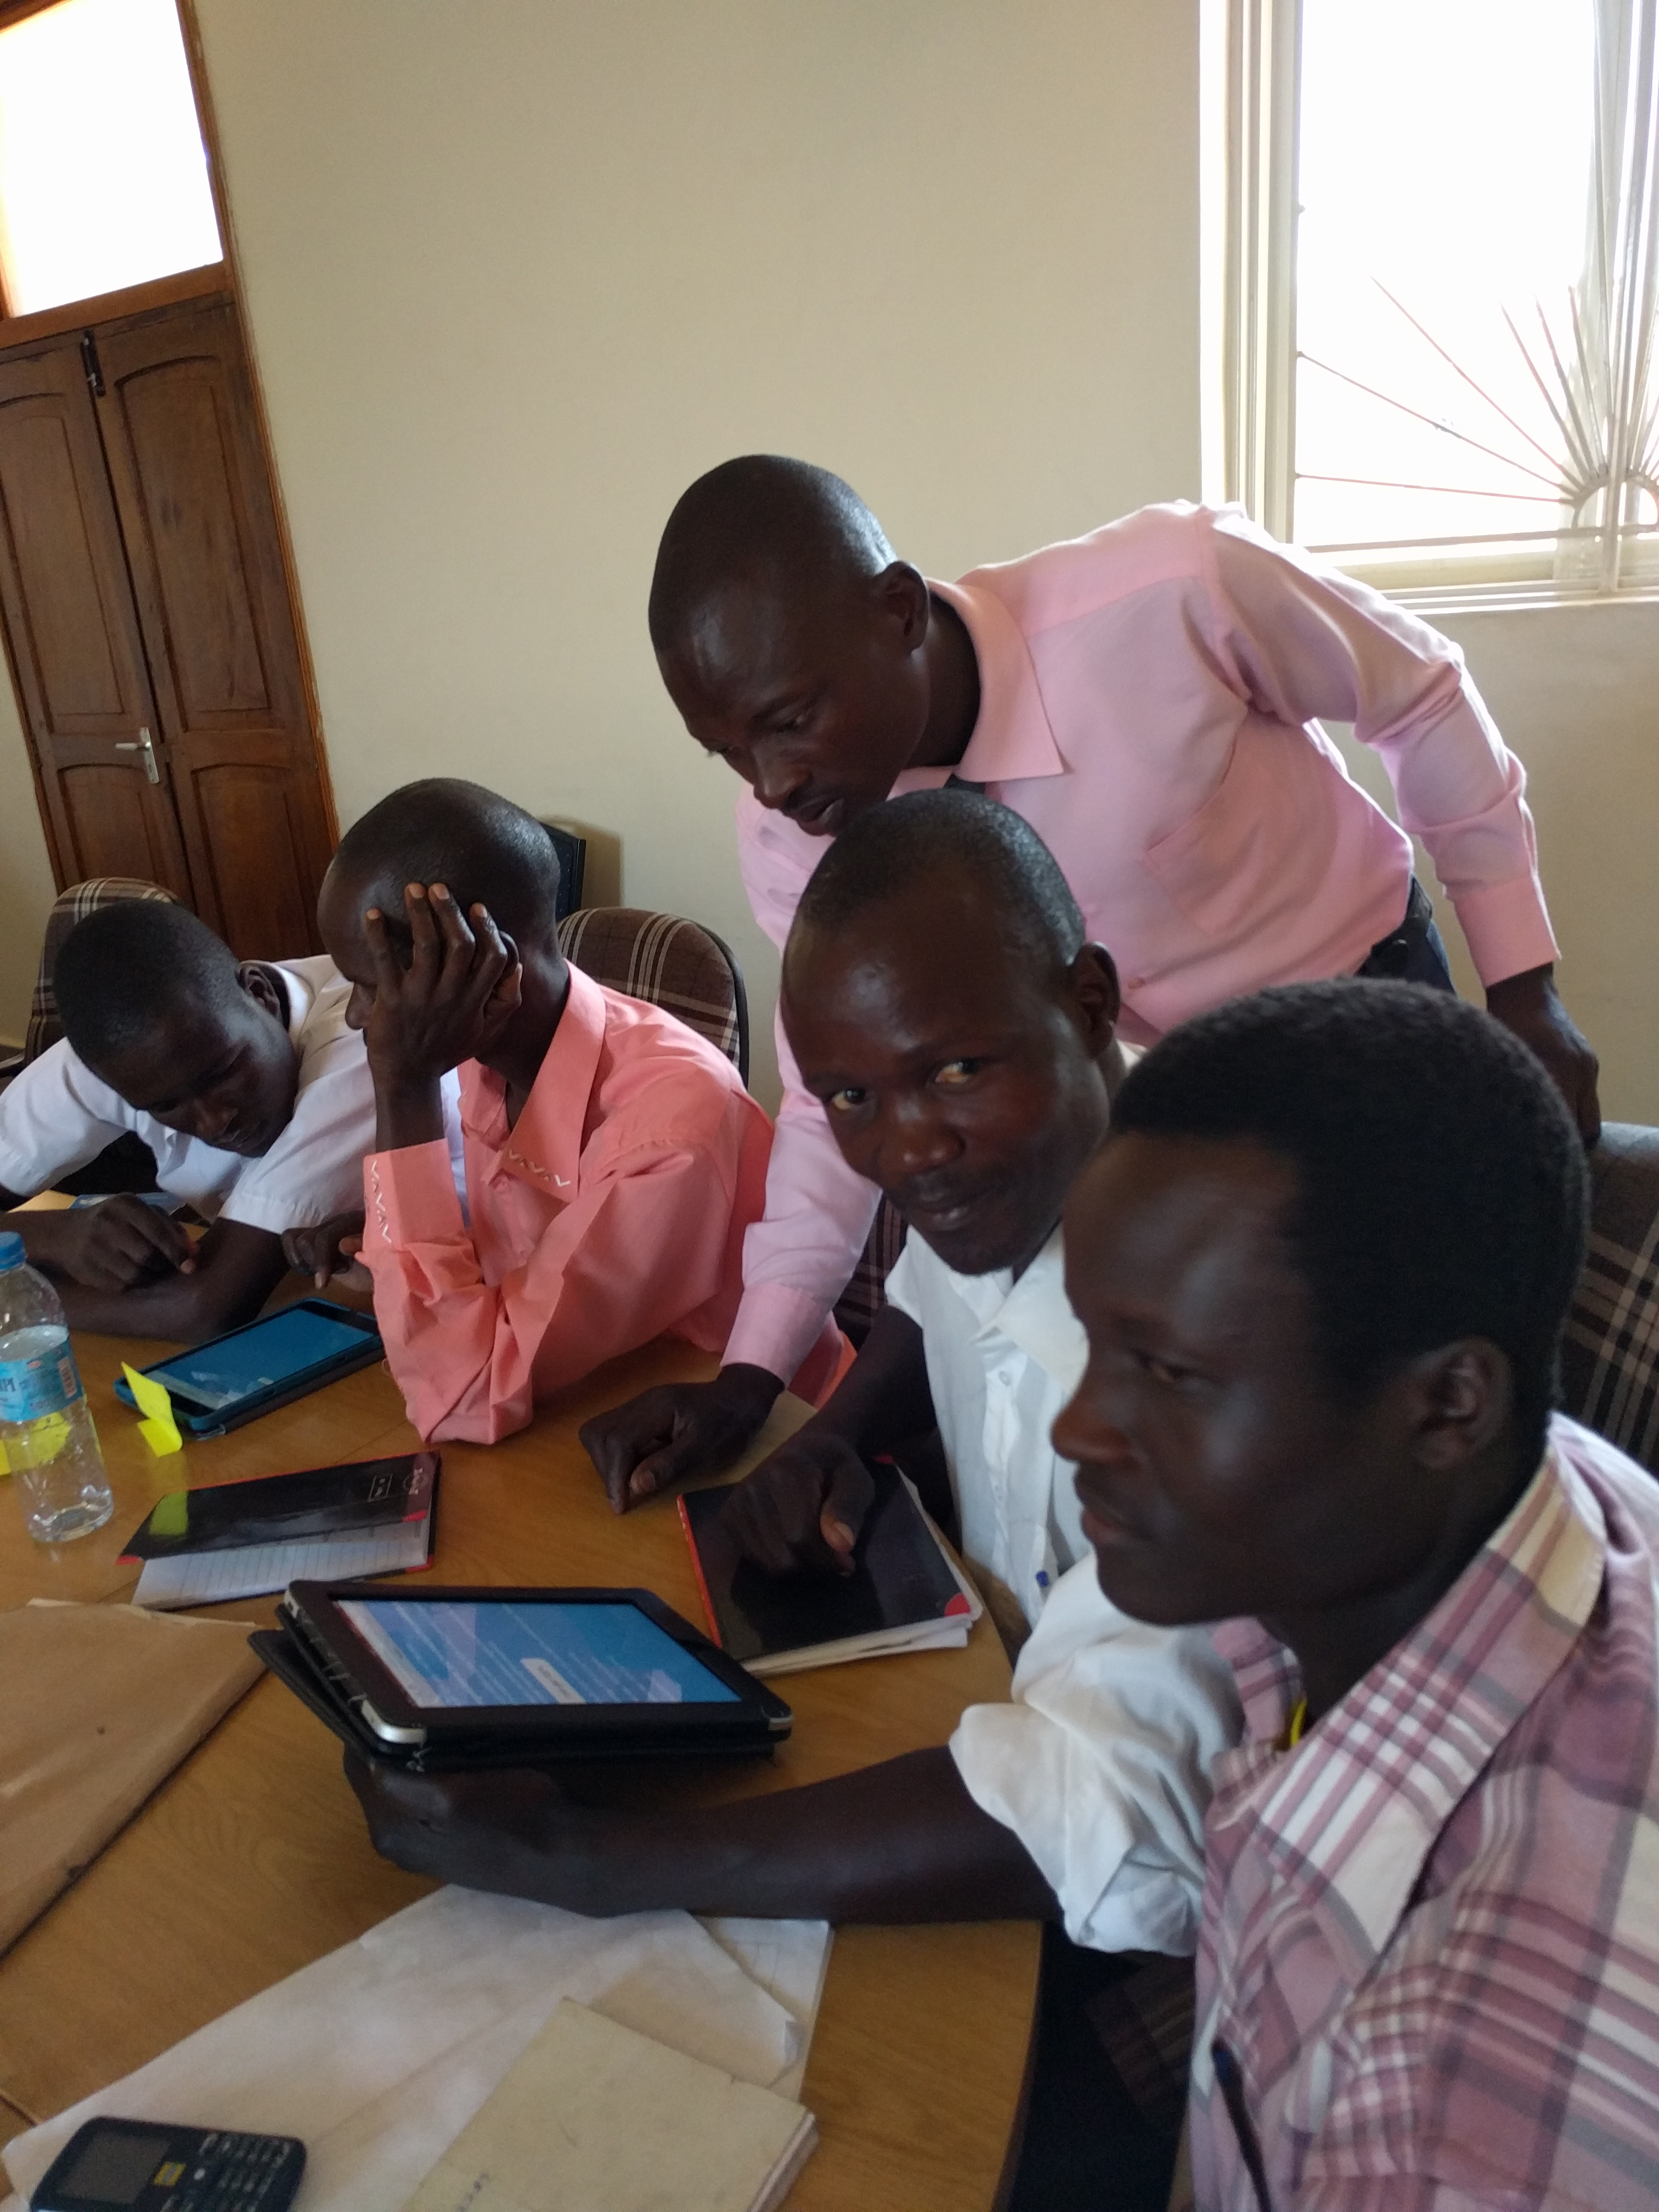
\includegraphics[width=0.4\textwidth]{iteration3/appTestTablet.jpg}
    \caption{Two coaches using a tablet for the formative app test. The coaches worked in pairs. After the app test, interviews was held, before co-creation workshops started.}
    \label{fig:tabletTest}
  \end{figure}

  \begin{figure}[h]
    \centering
    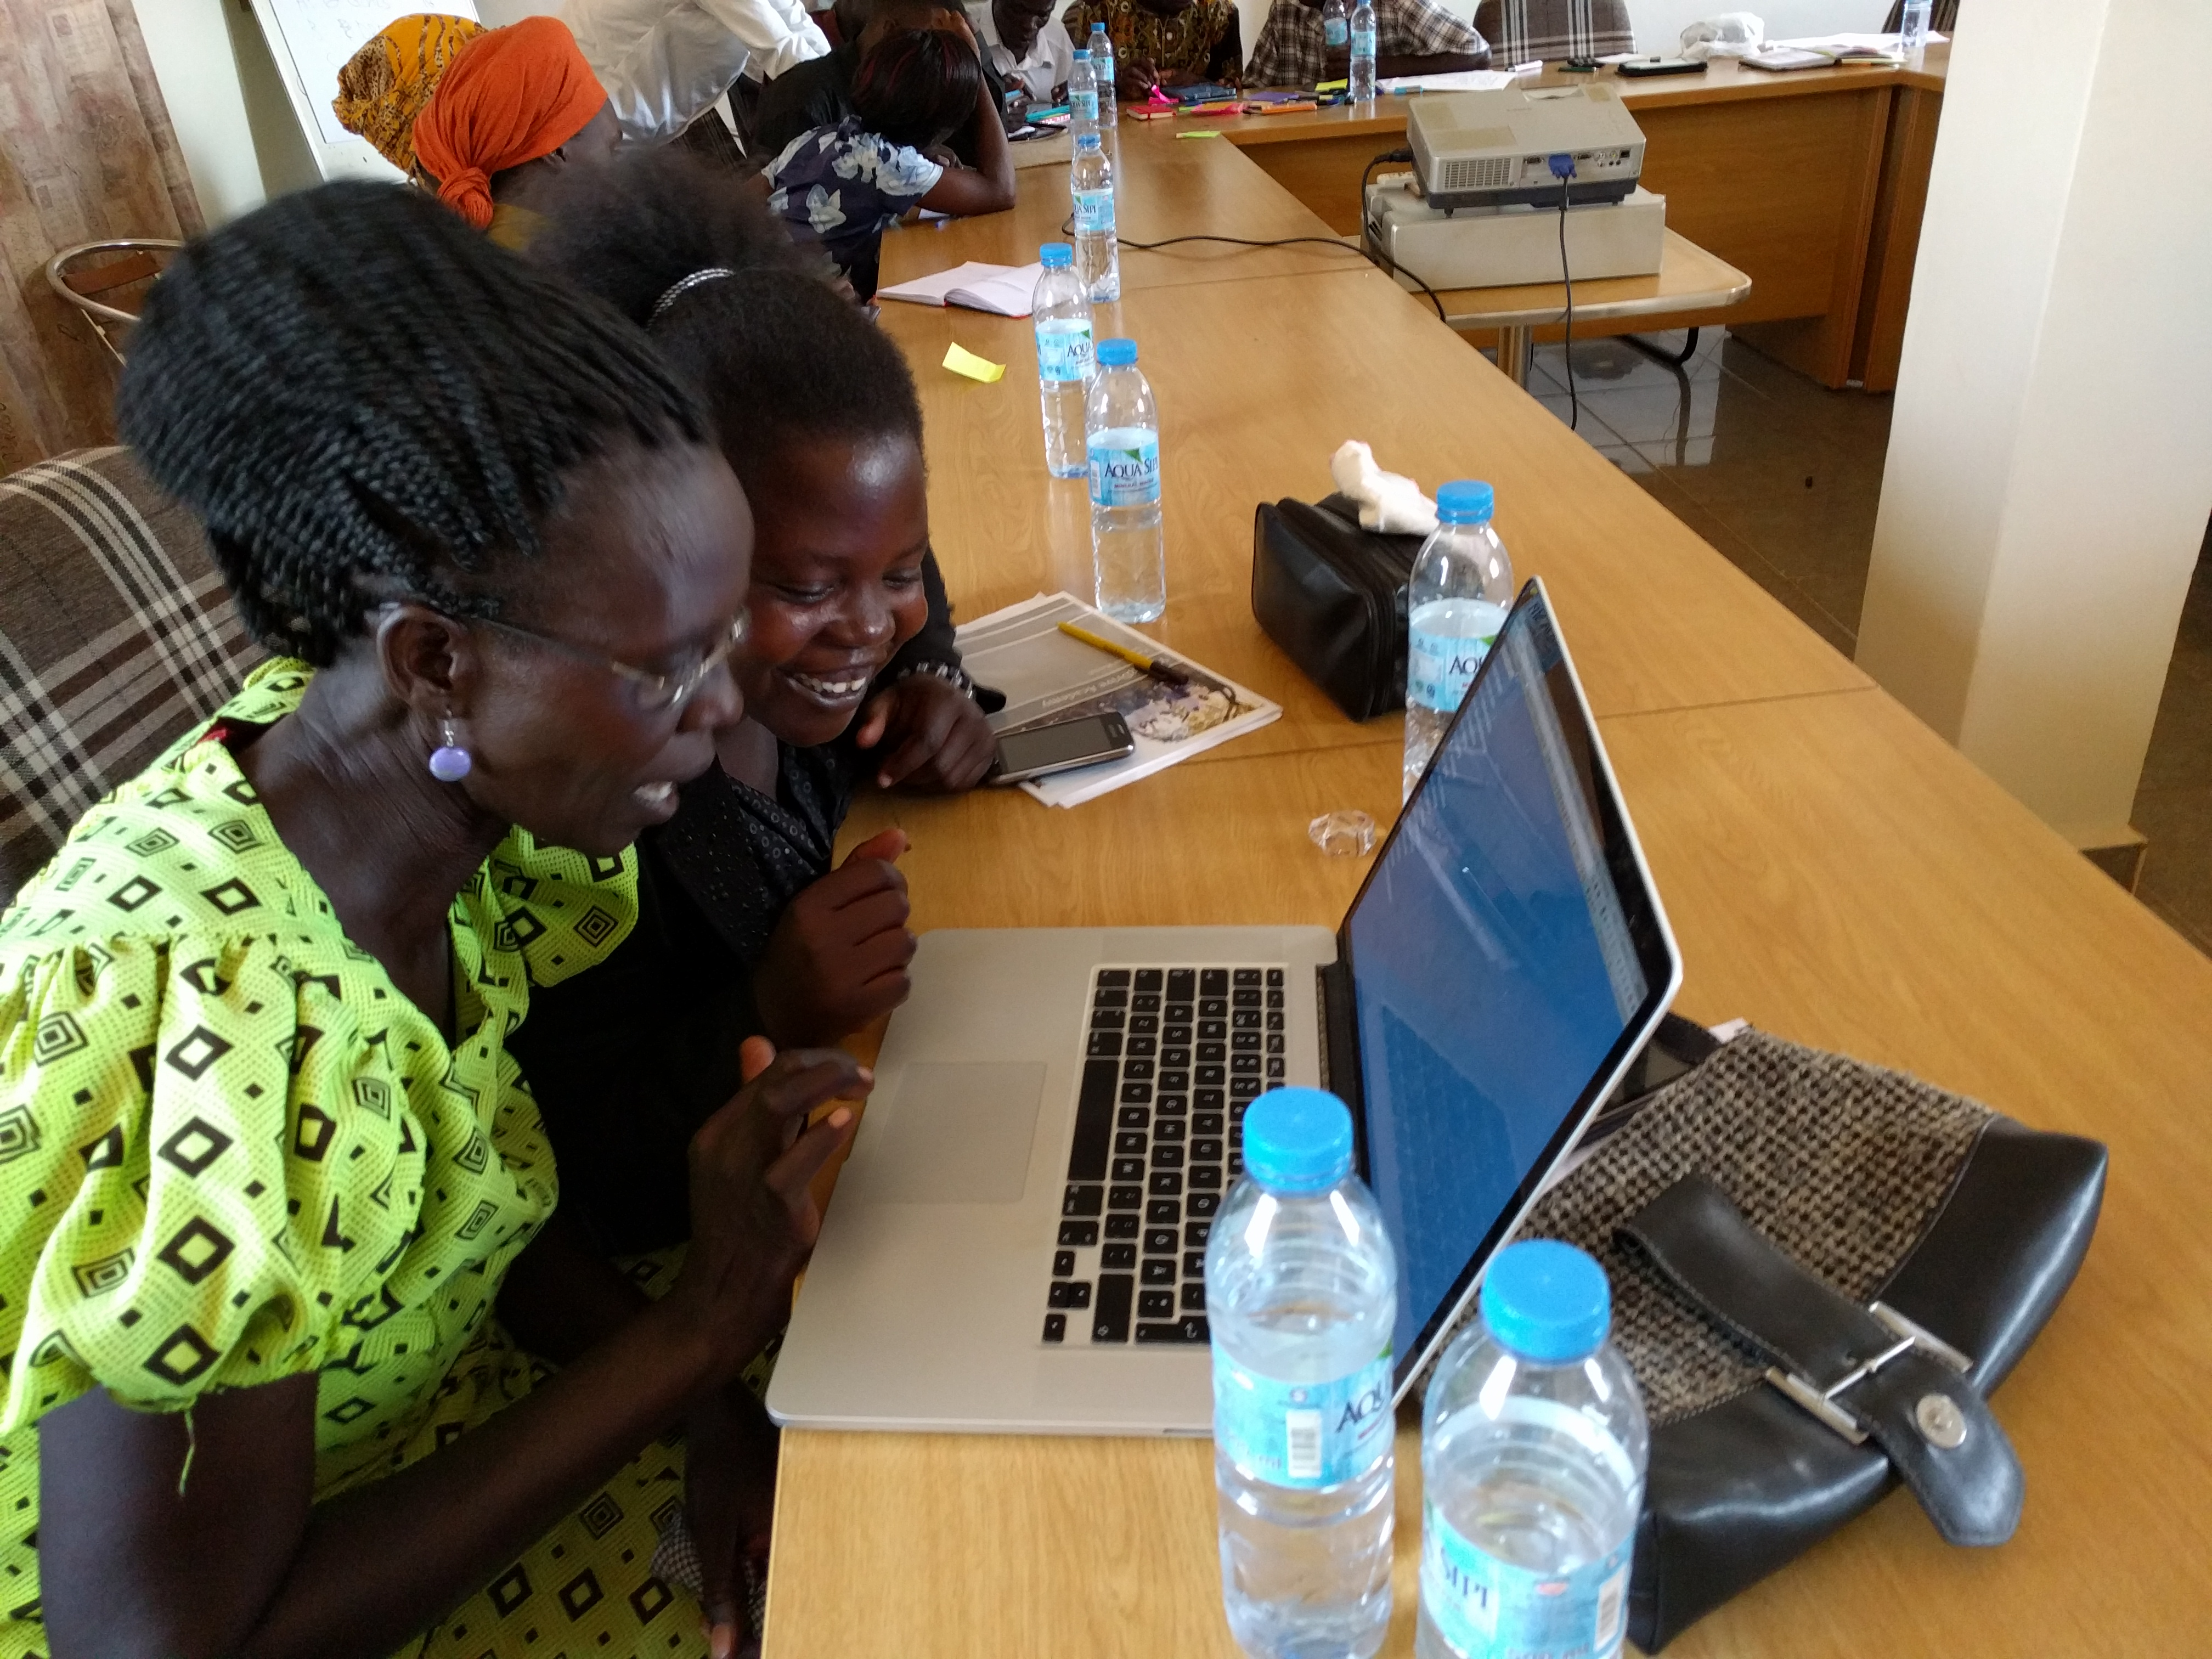
\includegraphics[width=0.8\textwidth]{iteration3/appTestComputer.jpg}
    \caption{A variation of smartphones and tablets were used. In one case, the battery died on one of the device so it needed to be replaced with a computer. It was the first time the coaches used a computer, and they learned quickly and eagerly.}
    \label{fig:computerTest}
  \end{figure}

  Regarding usability, the most negative thing from the app test, was that the app was not user friendly for first-time smartphone users. There were a lot of bugs, the most damaging for the app test being resizing of the font size for each new question, see figure \ref{fig:iteration-map} E-3. This forced some coaches to try to zoom on the devices, even if they did not know how. This could in turn cause refresh of the web page, and sometimes there was no Internet available. Thus, the data can not be fully reliable.

  This was the first time true frustration was shown. Out of 23 respondents, 7 rated the app easy, 11 medium, and 6 hard. This was not viable.

  Another reason for this, is that cognitive load seemed to be too high. The feedback was not scaffolded enough, so coaches did not have enough energy to assess all of their results carefully before taking the test again via "Improve". One user did not want to press "Improve" until having read the manual. The motivation was: "Not because that is what the info says, but because I can learn more from the manual, about more than what the questions says." This is in fact the preferred behaviour from Josefina, and the app should continue to further encourage only using the app training or certification mode after having prepared via the manual. This way, the app is still assessment, but it is "learning by thinking", with feedback. In iteration 4, comparing those that are allowed to use the manuals with those that are not allowed to, would be interesting.

  Regarding learning, four new ideas were tested during the app test, assessing the new pedagogical model of the app. Item 1-3 were tested in the app (the high-fidelity trigger material), and item 4 was tested via low-fidelity trigger material, asking a coach (and then the coach audience) if he or they could give the answers from memory without being shown alternatives.

  \begin{enumerate}
  \item "Try again"-button. When clicked, your wrong answers are repeated.
  \item If 100\% on the 1st try, gold. On 2nd try: silver. On 3rd try: bronze.
  \item Ask meta-cognitive questions, "Are you sure?", at the end of each question.
  \item Record your answer to the question before you are shown alternatives.
  \end{enumerate}

  Item 1, 2 and 3 were determined good after the interviews. Item 4 showed relevance, but implementation in the app would give many challenges (mainly how to assess if the coach could give the right answer without giving different alternatives. Voice recognition or free-form answers are hard to analyze, to implement, and to use by a first-time smartphone user).

  \clearpage

\subsection{Follow-Up Co-Creation Workshops}

  There were room for doing five co-creation workshops during iteration 3, which were done immediately after the big app test with the same 25 coaches. For the following workshops, the coaches themselves could propose topics. These were the five suggested topics by the coaches:

  \begin{enumerate}
  \item Finding the YoungDrive icon after unlocking the device
  \begin{itemize}
    \item The outcome led to in iteration 4, only the YoungDrive icon being on the start screen, and no other apps.
  \end{itemize}
  \item Making the app more user-friendly
  \begin{itemize}
    \item While the proposals was not very concrete, this led to a realization that the app needed to be more user-friendly, and thus gave a larger focus on this for iteration 4.
  \end{itemize}
  \item Finding local examples of entrepreneurs to inspire the youth
  \begin{itemize}
    \item This lead to the realization that most coaches having a hard time finding local success examples of entrepreneurs. An app could address this need in the future, both having a bank of successful local entrepreneurs, and booking them for visiting a youth session.
  \end{itemize}
  \item How to get access to smartphones (costing no more than ~70 USD)
  \begin{itemize}
    \item The action was very concrete: a Plan International staff voluntarily participated in this workshop, they contacted two retailers of smartphones, and concluded that 1) coaches could utilize the youth saving group to afford buying their own devices or 2) Plan International could buy and then borrow devices to the coaches, coaches being prepared to pay if they got lost or damaged. The results showed that both stakeholders and coaches are very eager to be equipped with smartphones, seeing the benefits.
  \end{itemize}
  \item Becoming a better coach via other apps (like Google's products)
  \begin{itemize}
    \item This workshop was very interesting, as coaches found numerous uses of a smartphone which would benefit them in their work. The coaches even figured out how to use Google voice to ask questions, like the most profitable company in Tororo, or getting directions, or using the app for translations. It is evident that equipping the coaches with smartphones has very concrete extra benefits other than the YoungDrive app, and shows a tendency that the coaches are more eager to use the smartphone for utility than for entertainment.
  \end{itemize}
  \end{enumerate}

\subsection{App Tests with Three Coaches Before and After a Youth Session}

Below, the results from the app tests with three coaches before and after having a youth session are shown.

  \subsubsection{App Test with Coaches Before a Youth Session: Collection of Affective Reactions, and Proposals for Improvements}

  There were three coaches testing the app after having prepared for their youth session, but before carrying out the teaching. Some things were notable from the field visits: %with John:
  \begin{itemize}
    \item "Are you sure?" is understood intuitively (you can't progress without answering), but some coaches deliberately answer "Yes" even if they are not sure.
    \item Idea to highlight different words of similar answers, to increase speed
    \item In summary, if wrong, show the other alternatives either way, not only the wrong answer
    \item Idea for future work: "Go to participant manual" within the app % Juliet, this was discovered:
    \item If correct and unsure, she says "I still feel good". "Include it in wrong, because maybe I was still guessing".
    \item Change button to "Become certified", to increase likelihood to press the button. As of now, it was not obvious.
  \end{itemize}

  When she did get certified, she said: "I feel good". When asked why, she said: "They have appreciated what I have done". The next day, the same three CBTs gathered at the Plan International office to do an app test on the hardest quiz.

  Having a service mini-sprint after the field visit, quick iterations could be made to the app. One such example comes from the field visits. Originally, it was believed best to use Gold/Silver/Bronze in the Training mode, and "Are you sure?" in the Certification mode. User tests showed that the other way around was better, and this was changed for the next meeting with the coaches. This example shows the relevancy of testing the app with the intended users, as it had not been evident from the tests with the Kampala student or the teacher.

  A service design approach was used, first observing how preparations was made without the app, and \textit{then} introducing assessment via the app, followed by interview. What was the most valuable feedback from the field visits, was to see that the app had indeed been a perfect fit for use in the field before a youth session. However, it was not possible due to time limitations to follow the coach to their youth session afterwards, to see the actual effect of preparing via the app.

  \subsubsection{App Test with Coaches After the Youth Session: Quiz Results and Analysis}

  Several conclusions could be drawn the day after from a joined app test with the same three coaches from the field visits. Two of the coaches were competing with finishing the coach guide quiz 9 (see results in figure \ref{fig:areYouReady}, the coach guide quiz for the topic they had taught the day before. The third coach (who arrived late) offered feedback on the app.

  \begin{figure}[h]
    \centering
    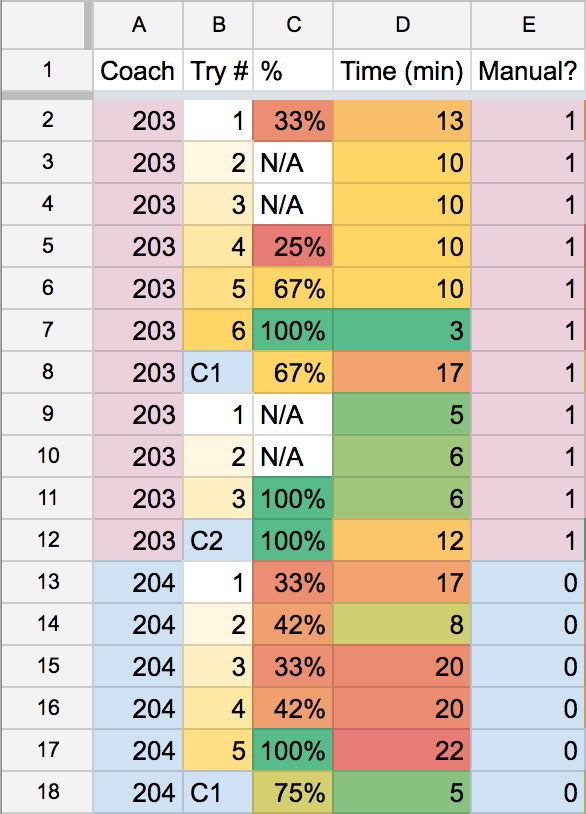
\includegraphics[width=0.5\textwidth]{analysis/sheets/iteration2tororo_smalltest_compressed.png}
    \caption{Data analysis in Google Sheets from the quiz results during the workshop for the coach guide quiz 9: "Are you ready?". It is observed how the two coaches (id 203 and 204) scores for each new try, where C1 means "Certification try 1". N/A means that the quiz score were not logged at this specific time. "Manual?" means that if 1, the manuals could be consulted.}
    \label{fig:areYouReady}
  \end{figure}

  \clearpage

  The two coaches did 17 quiz tries on quiz 9. Coach 203 (referred to as "Beatrice" in the text) was allowed to use the manual, while coach 204 (referred to as "Rehema" in the text) could only consult the feedback via the app, see figure \ref{fig:iteration-map}, D-3 and H-3.

  Apart from the quantitative quiz results, some comments were made. Beatrice having 4/12 correct answers on the first question, when asked from the quiz question 13 "How comfortable and ready do you feel right now to carry out session 9? (There is no right answer, just be honest with yourself!)", answered " Ready, but I probably still want to look in the coach manual and participant manual.". The other alternatives were: "Not ready at all, I need to prepare myself more by using the coach manual and participant manual.", "Somehow ready, but I still need to look more in the coach manual and participant manual." or "Very ready and comfortable.".

  Beatrice got 4/12 correct answers on her first try, but eventually she did pass the certification, getting 12/12 correct answers in one try in 102 minutes from the quiz start. It took her 43 minutes from her quiz try 1 to passing the training. She then failed the certification try 1 (i.e. not getting Gold) after spending 17 minutes with it. Thus, she needed to go back to the training. Back in the training, now she got 8/12 instead of 4/12, and passed the whole training in 17 minutes. Then, she got 12/12 in the certification test (earning Silver), in only 12 minutes.

  Rehema also got 4/12 correct answers on her first try. Not understanding the "Improve" button, she repeatedly went back to the home screen and retook the whole test (like in iteration 2). This was a slow approach. On her new tries, she got 5/12, 4/12, 5/12, which showed that learning was too hard. Similar results had been found in iteration 1 using Duolingo, where the app failed to train the coach to get a better score. After this try, she was explained the "Try again" button, got 7/7 (spending 22 minutes with the questions compared with her 16.25 minutes average doing all 12 questions, which showed she really put effort into analyzing the answers properly). Unlocking the certification test, she got 9/12 in 5 minutes, an improvement from 4/12 on her quiz try 1 75 minutes before.

  The results from this quiz shows that:
  \begin{itemize}
  \item "Improve", only needing to repeat the questions you are not sure of, does improve learning quality and speed, compared to retaking the whole quiz again after each try - it makes learning more focused on what you need to train
  \item It needs to be clearer that you should press "Improve", for example by changing the text to "Try again"
  \item The time needed to become reliant on the session takes too long. To pass the rule of thumb for deliberate practice, a session getting to 95\% reliability should take 45-90 minutes. For Beatrice, it took 102 minutes from quiz start to being 100\% reliable. For Rehema, she did only manage to get 75\% reliable within the same time frame. Either scaffolding needs to increase (dividing the quiz into smaller chunks), or learning effectiveness needs to increase (for example by better feedback).
  \end{itemize}

The data and observations also shows that learning Correct Structure and Time Management via multiple-choice is not effective. Especially, this is shown by the time it takes to get a high score. To score well on such a test, the coach would retrieve from memory using a clear mental image. In its current design, getting a clear mental picture is not supported by the multiple-choice design. See Future Work in chapter \ref{cha:future-work} for a further discussion how this Correct Structure and Time Management can be better assessed in the future.

\subsection{Discussion}

  For iteration 3, the coaches could not only assess, but also \textit{learn} Correct Information, which was successful, but needs to be done more effectively. It took an unacceptable amount of time to reach 100\% proficiency on all the quizzes. This was especially evident, on the quiz on Correct Structure och Time Management, "Week 9: Are you ready?", when it took a coach 102 minutes to reach 100\% without errors. In iteration 2, when "Improve" did not exist, it probably would have taken even longer.

  For the first time both signs of learning via perceptual exposure (many questions during a limited time, by trial and error) and deliberate practice (via learning via reflection) could be identified from the app. It is just that the app as of now is quite inefficient, especially in terms of speed, so while the ideas are there, the criteria are not fulfilled.

  The focus had been on "I am well prepared", but also including "I am certified.". It was shown that most coaches does not care about the simple gamification aspect of "I am certified" (which the workshop already had shown) but that they do care about their learning progress and learning results. The app could further embrace this.

  If there is one thing additional learned during the iteration, it is the notion of "data is knowledge, and knowledge is power". A realization is that both the developer, the coaches, the teacher, and the project partners can gain important insights. Adding "Are you sure?" to each quiz question, coach understanding was amplified, because now, also the coach's attitude towards learning can be evaluated. See more about this in the Discussion chapter \ref{cha:discussion}.

  \subsection{Next iteration}
  To improve effectiveness for the next iteration, a couple of goals were chosen. While the app would work well for the Ugandian coach training, the use case of a youth session was not good enough yet. Mostly, this is in regards to that it takes too long time to improve via the app, and that the feedback is not sufficient.

  \begin{itemize}
    \item Improve Deliberate practice. The criteria for Deliberate practice is not fulfilled today.
    \begin{itemize}
      \item  Follow the recommendation to design so that knowledge in a topic can go from unreliable to 95\% reliability within one to three 45-90-minute sessions.
      \item If this is not possible from changing the learning tactic, don't continue trying: split the quizzes into smaller pieces \citep{sierra}.
    \end{itemize}
    \item Improve Perceptual expose
    \begin{itemize}
      \item Divide the learner's expertise according to \cite{sierra}, "Can't do", "Can do with effort", and "Can do effortlessly".
    \end{itemize}
    \item Increase the use of questions to prompt self-monitoring  and self-evaluation \citep{sitzmann}.
    \begin{itemize}
      \item Using "learning by thinking" and encouraging a growth mindset, can benefit reaching metacognitive skills on Bloom's revised taxonomy.
      \item Help the coach to analyze and evaluate its own learning, possibly improving faster in the app.
    \end{itemize}
    \item Improve feedback to reflect that the teacher does not want to encourage coaches to have their youth session before they are 100\% confident with the material
    \item Data collection needs to be online and needs to be individual
    \begin{itemize}
      \item To do it online means that there needs to be a database, but also a login, so individuals are traceable.
    \end{itemize}
  \end{itemize}


\section{Iteration 4: Uganda Summative Test}

Here the results from the qualitative and quantitative data for iteration 4 are shown together with conclusions. In these activities, there were 25 coaches present during both the app test and the interviews.

\subsection{Analysis of Quiz Results}

    %What the data said

    % Christine och Patrick berättade senare att i regel presterar Young Mentor lite bättre än CBT, enligt deras rakningar. (från iteratoin 1 - stämde detta?)

    % Relevans av att testa financial literacy: "Precis som med förra gruppen, verkar ekonomin vara det svåraste att förstå (dolda utgifter, hur gå med vinst), som youth." (från iteration 1)

% Important to be objective
% En diskussion om hur resultaten kan användas i praktiken är också i de flesta fall belysande och relevant i rapporter

% https://liu.se/ias/kontakta-oss?l=en

For the first time, automatic data collection was used, which increased the amount of quantitative data that could be analysed substantially. Below, the findings from each data analysis method are presented. There was one test group and one reference group, the difference being if they were allowed to consult the manuals or only use the feedback from the app.

\subsubsection{Quiz Results and Pre-Test Data Analysed in Google Sheets}
For results gathered and analysed within the Google Sheet, see figure \ref{fig:analysFarg3}. For a zoomed in version, see Appendix \ref{cha:appendix4}. Early observations from the pre-test data when inserted into Google Sheets was that a surprising number of cells were left blank. One user had not done the pre-test (see column for coach 220), where some had left questions unanswered (most commonly "Do you own a company?" (should have used the word "business"), plus "Hours of preperation" and "Occations for a youth session" (there is a tendency this might be because they were not proud of their answers, because of correlations with low quiz results).

\begin{figure}[h]
    \centering
    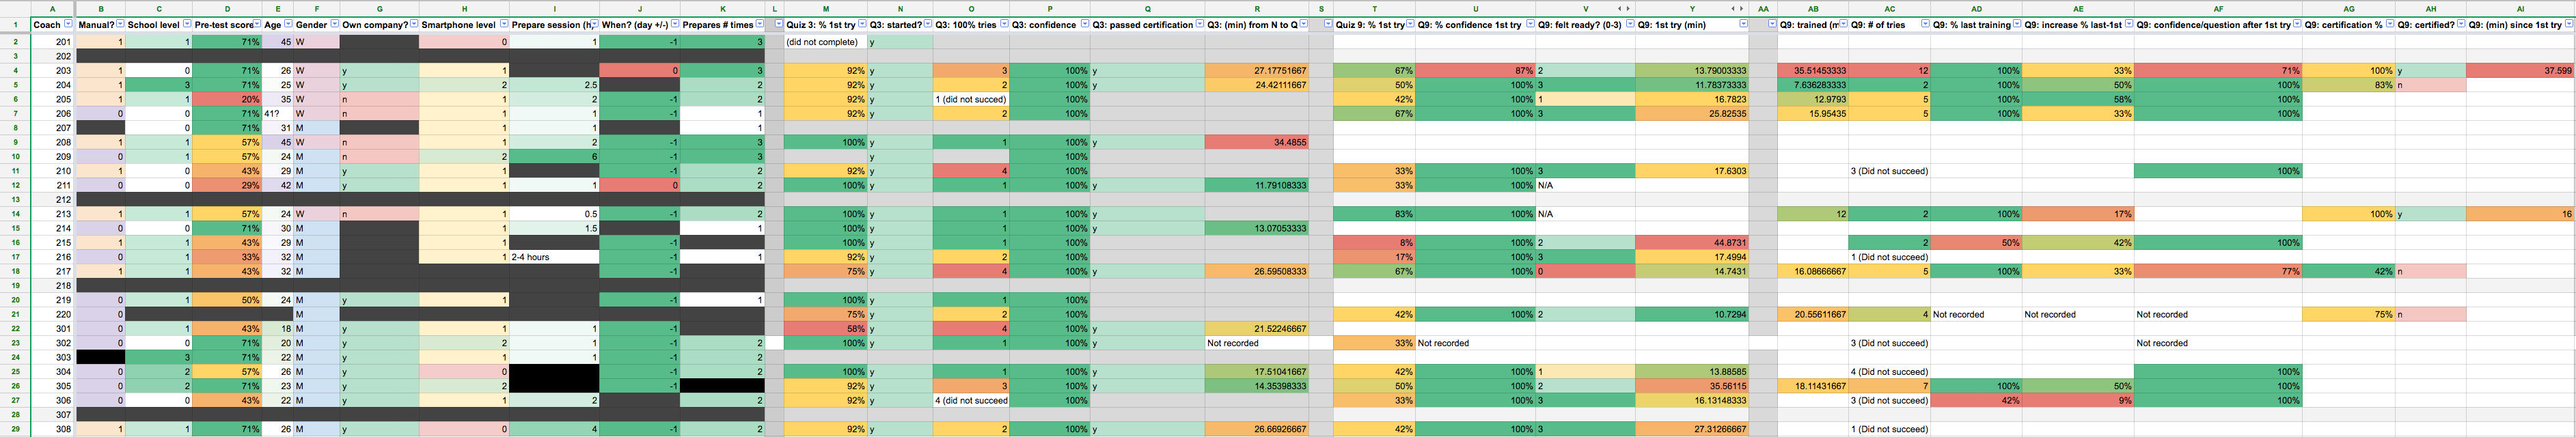
\includegraphics[width=1.0\textwidth]{analysis/sheets/0Overview.png}
    \caption{The Google Sheet after merging the pre-test data and the summed quiz results data. See zoomed-in versions and explanations for each section below.}
    \label{fig:analysFarg3}
\end{figure}

\begin{figure}[h]
    \centering
    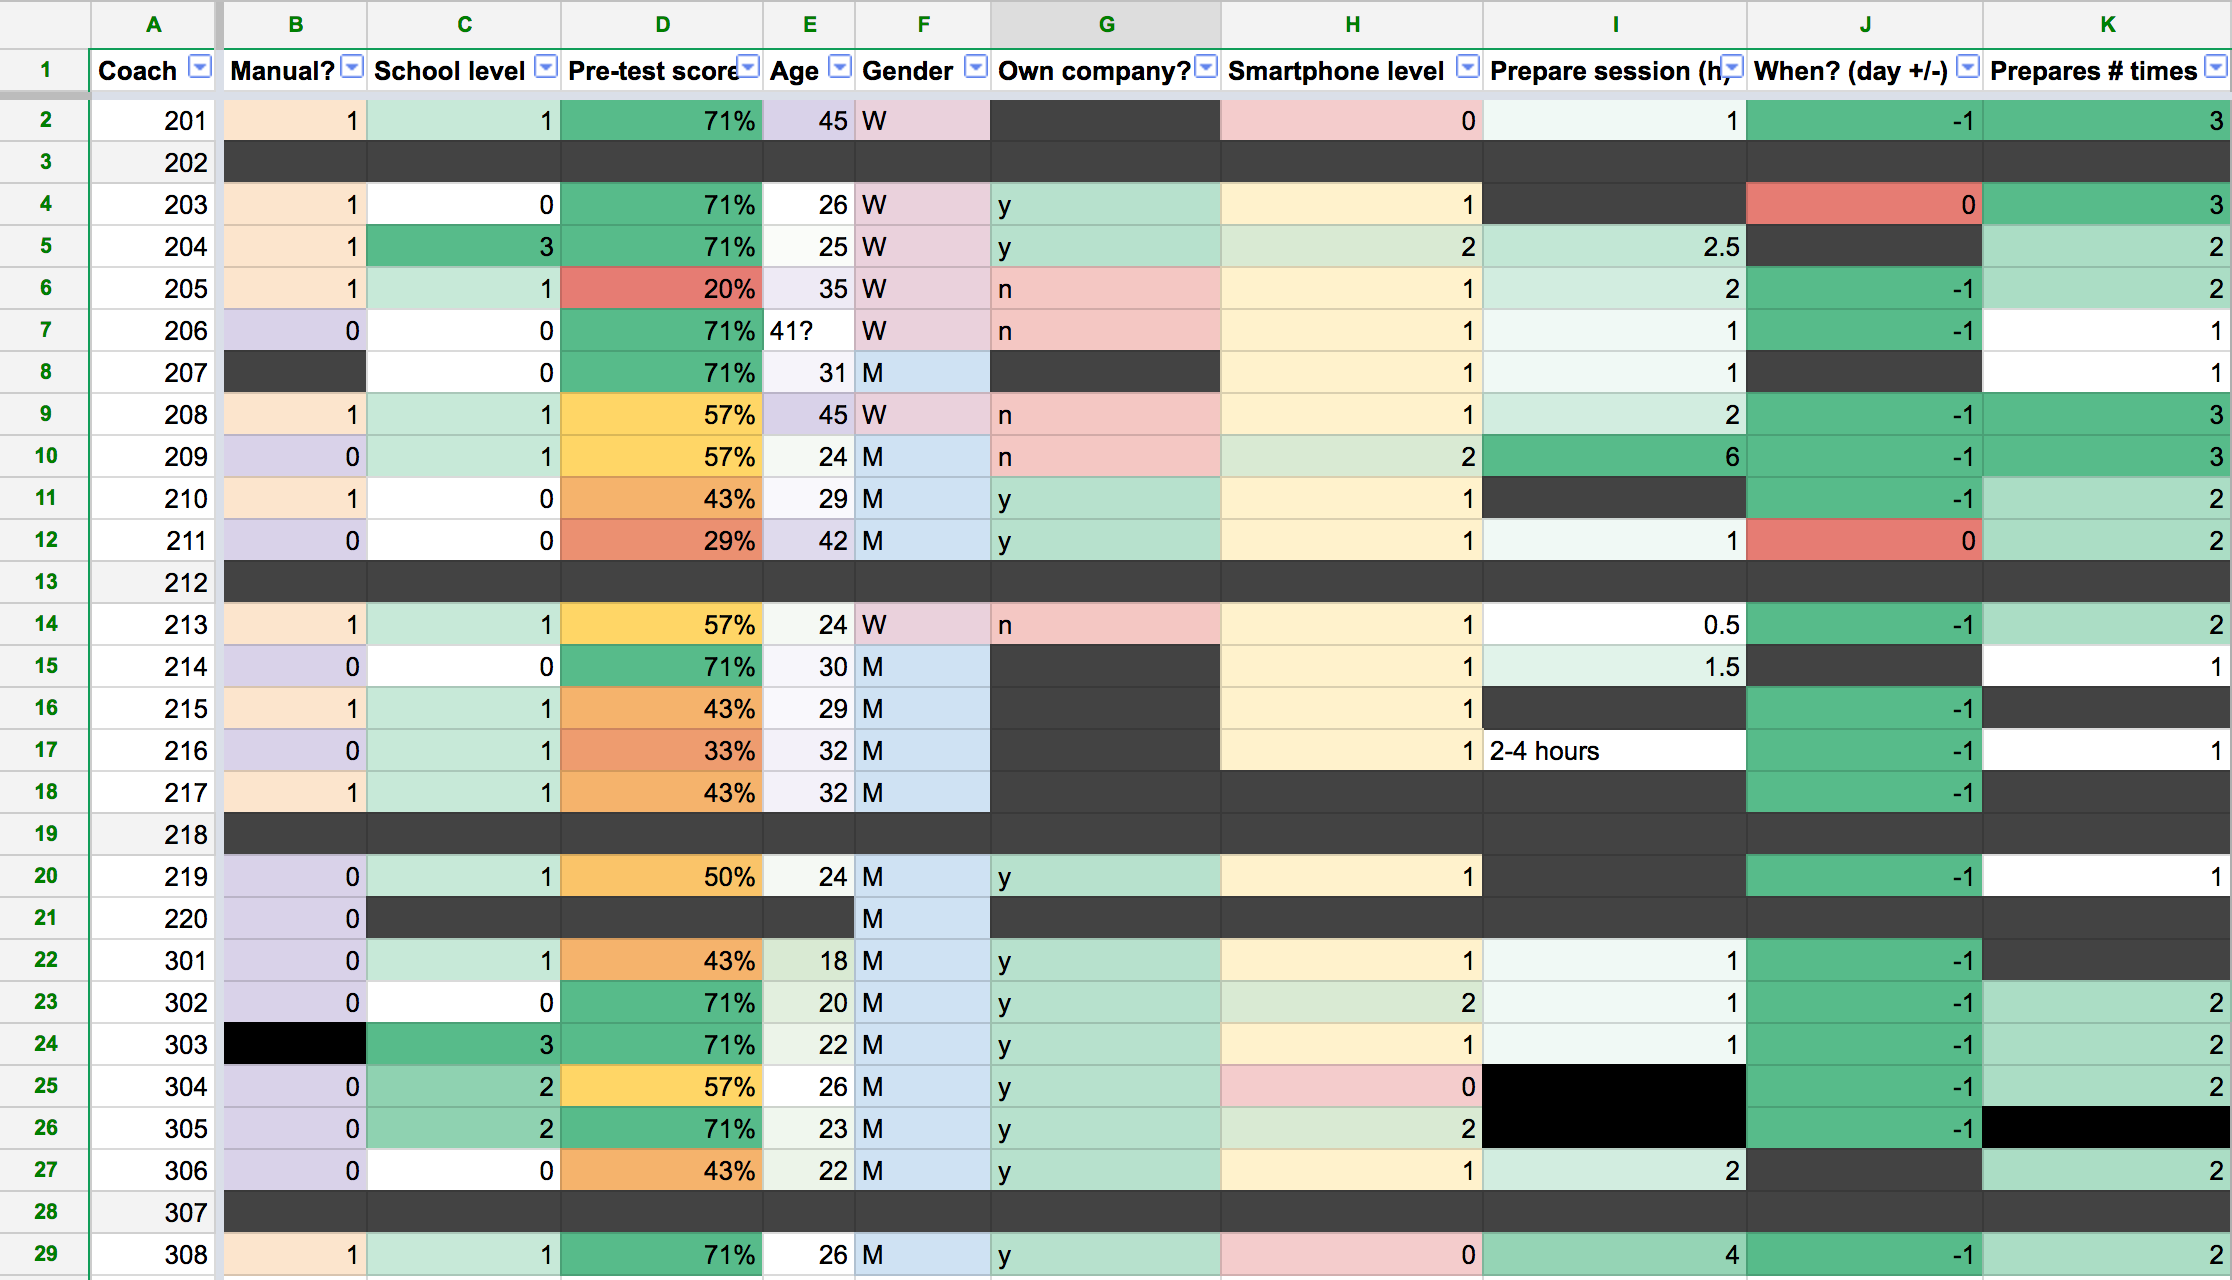
\includegraphics[width=1.0\textwidth]{analysis/sheets/1Pre-data.png}
    \caption{Pre-test data}
    \label{fig:1Pre-data}
\end{figure}

\begin{figure}[h]
    \centering
    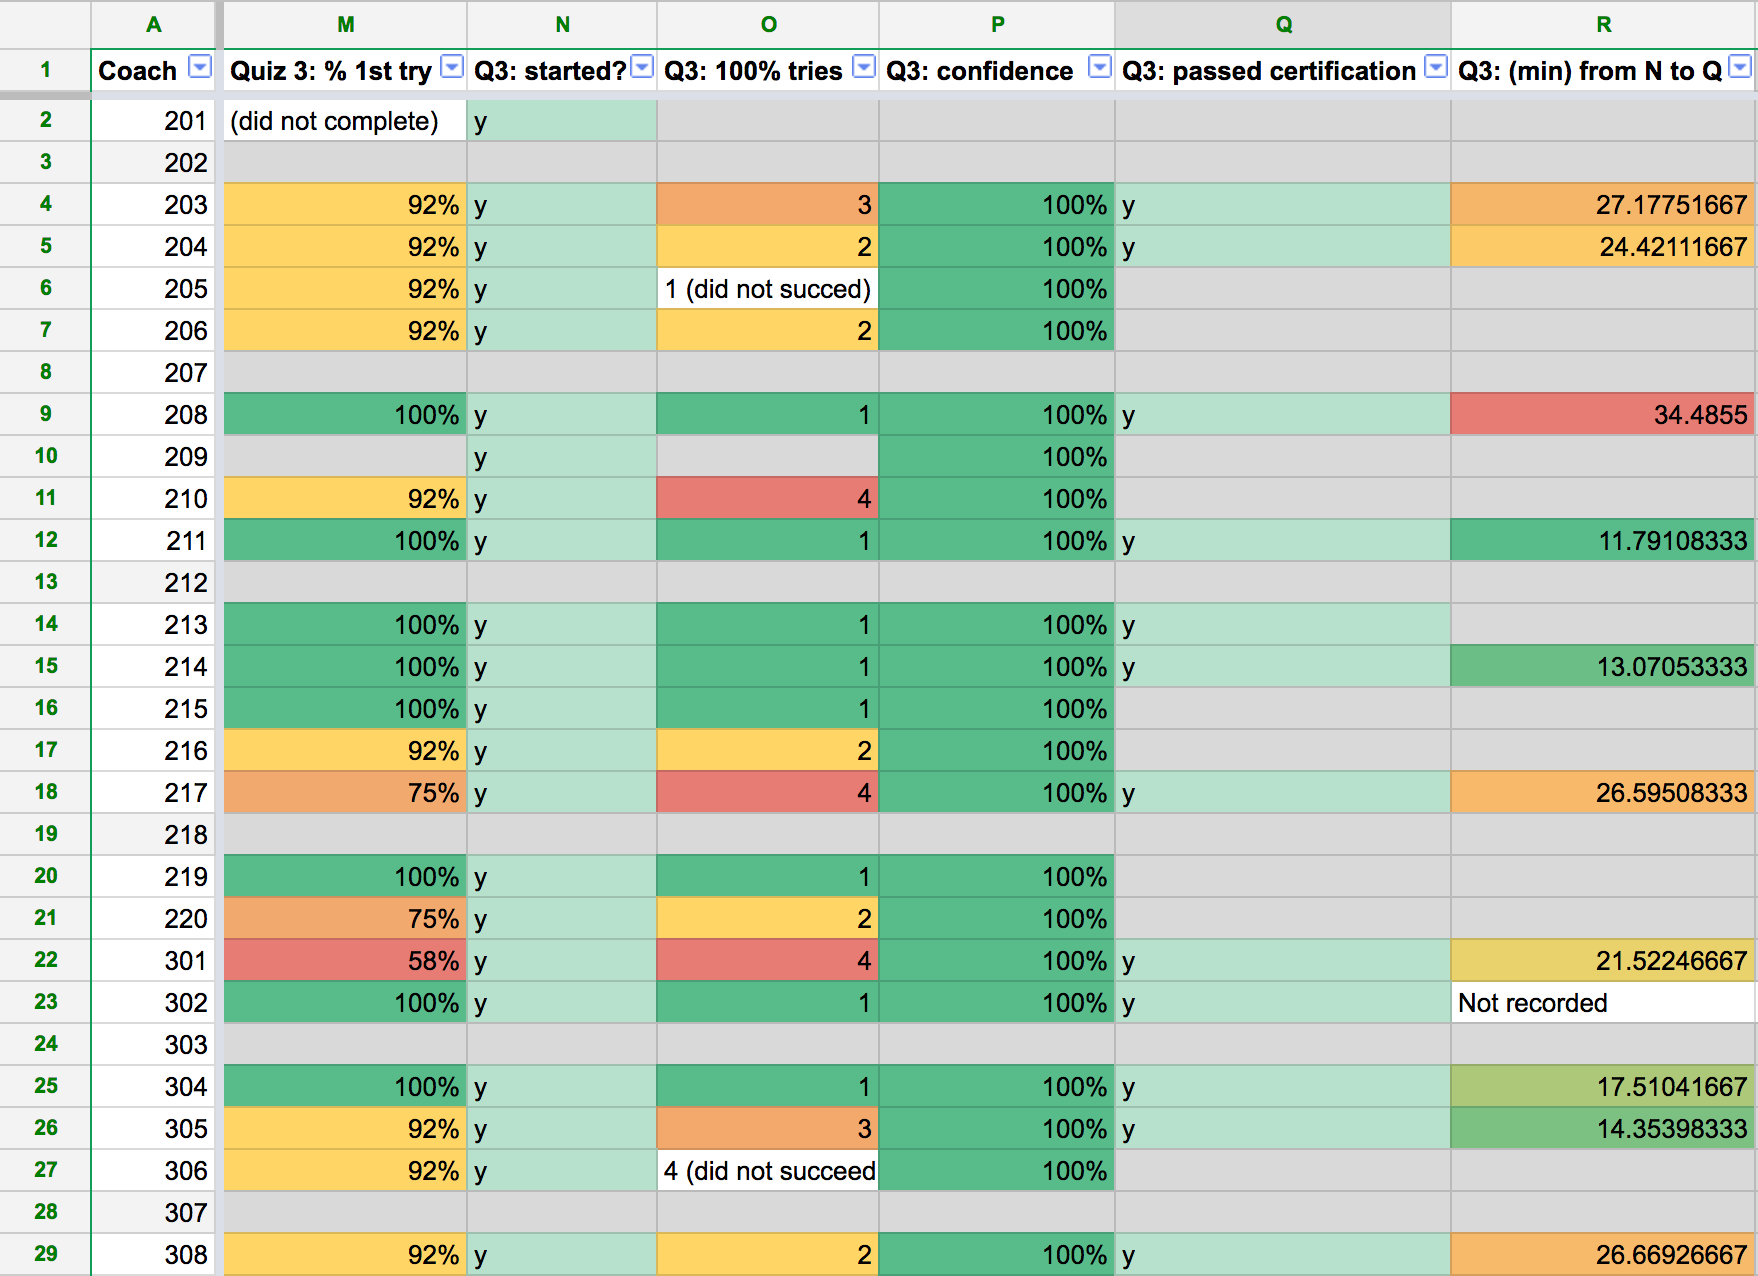
\includegraphics[width=1.0\textwidth]{analysis/sheets/2Quiz3.png}
    \caption{Quiz 3 answers.}
    \label{fig:2Quiz3}
\end{figure}

\begin{figure}[h]
    \centering
    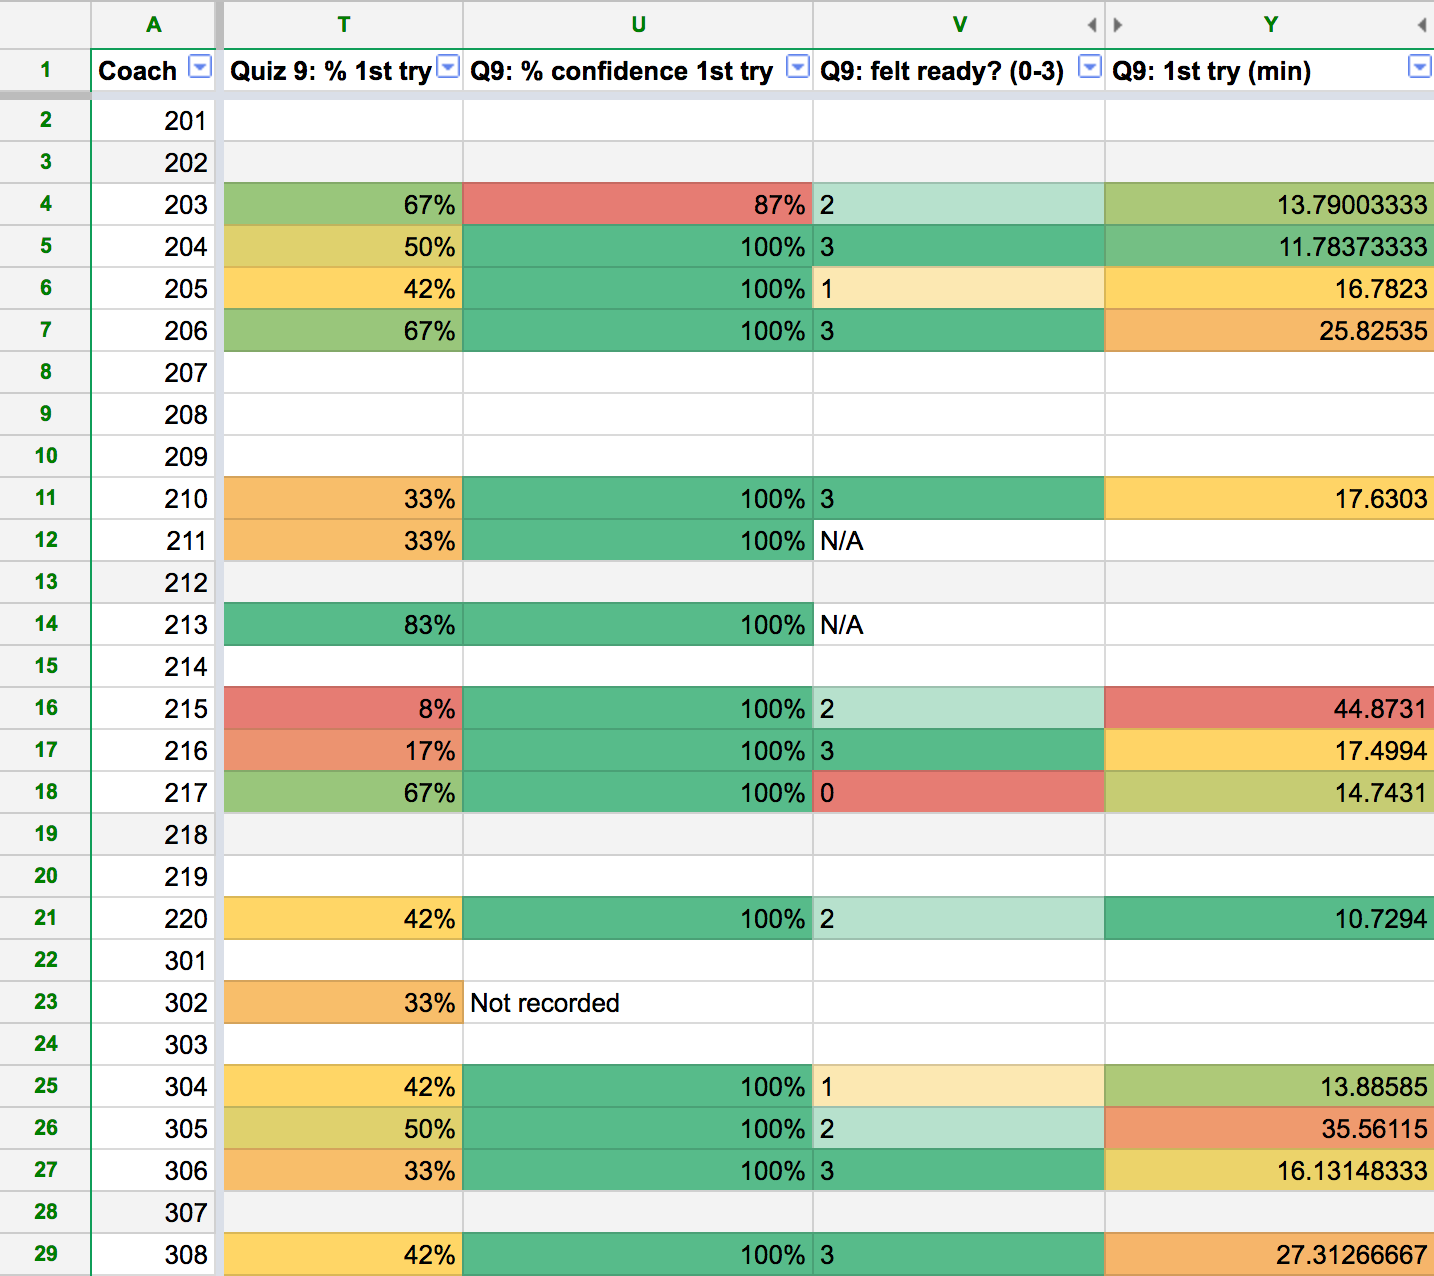
\includegraphics[width=1.0\textwidth]{analysis/sheets/3Quiz9A.png}
    \caption{Quiz 9 try 1 answers (correctness and recorded confidence ("Are you sure?": "Yes/No") on coach guide quiz 9 "Are you ready?", together with answering "How comfortable and ready do you feel right now to carry out session 9? (There is no right answer, just be honest with yourself!", alternative 1-4 ("Not ready at all", "Somehow ready", "Ready" or "Very ready and comfortable"). Finally in column Y, the time it took for the coach to complete quiz try 1 is given.}
    \label{fig:3Quiz9A}
\end{figure}

\begin{figure}[h]
    \centering
    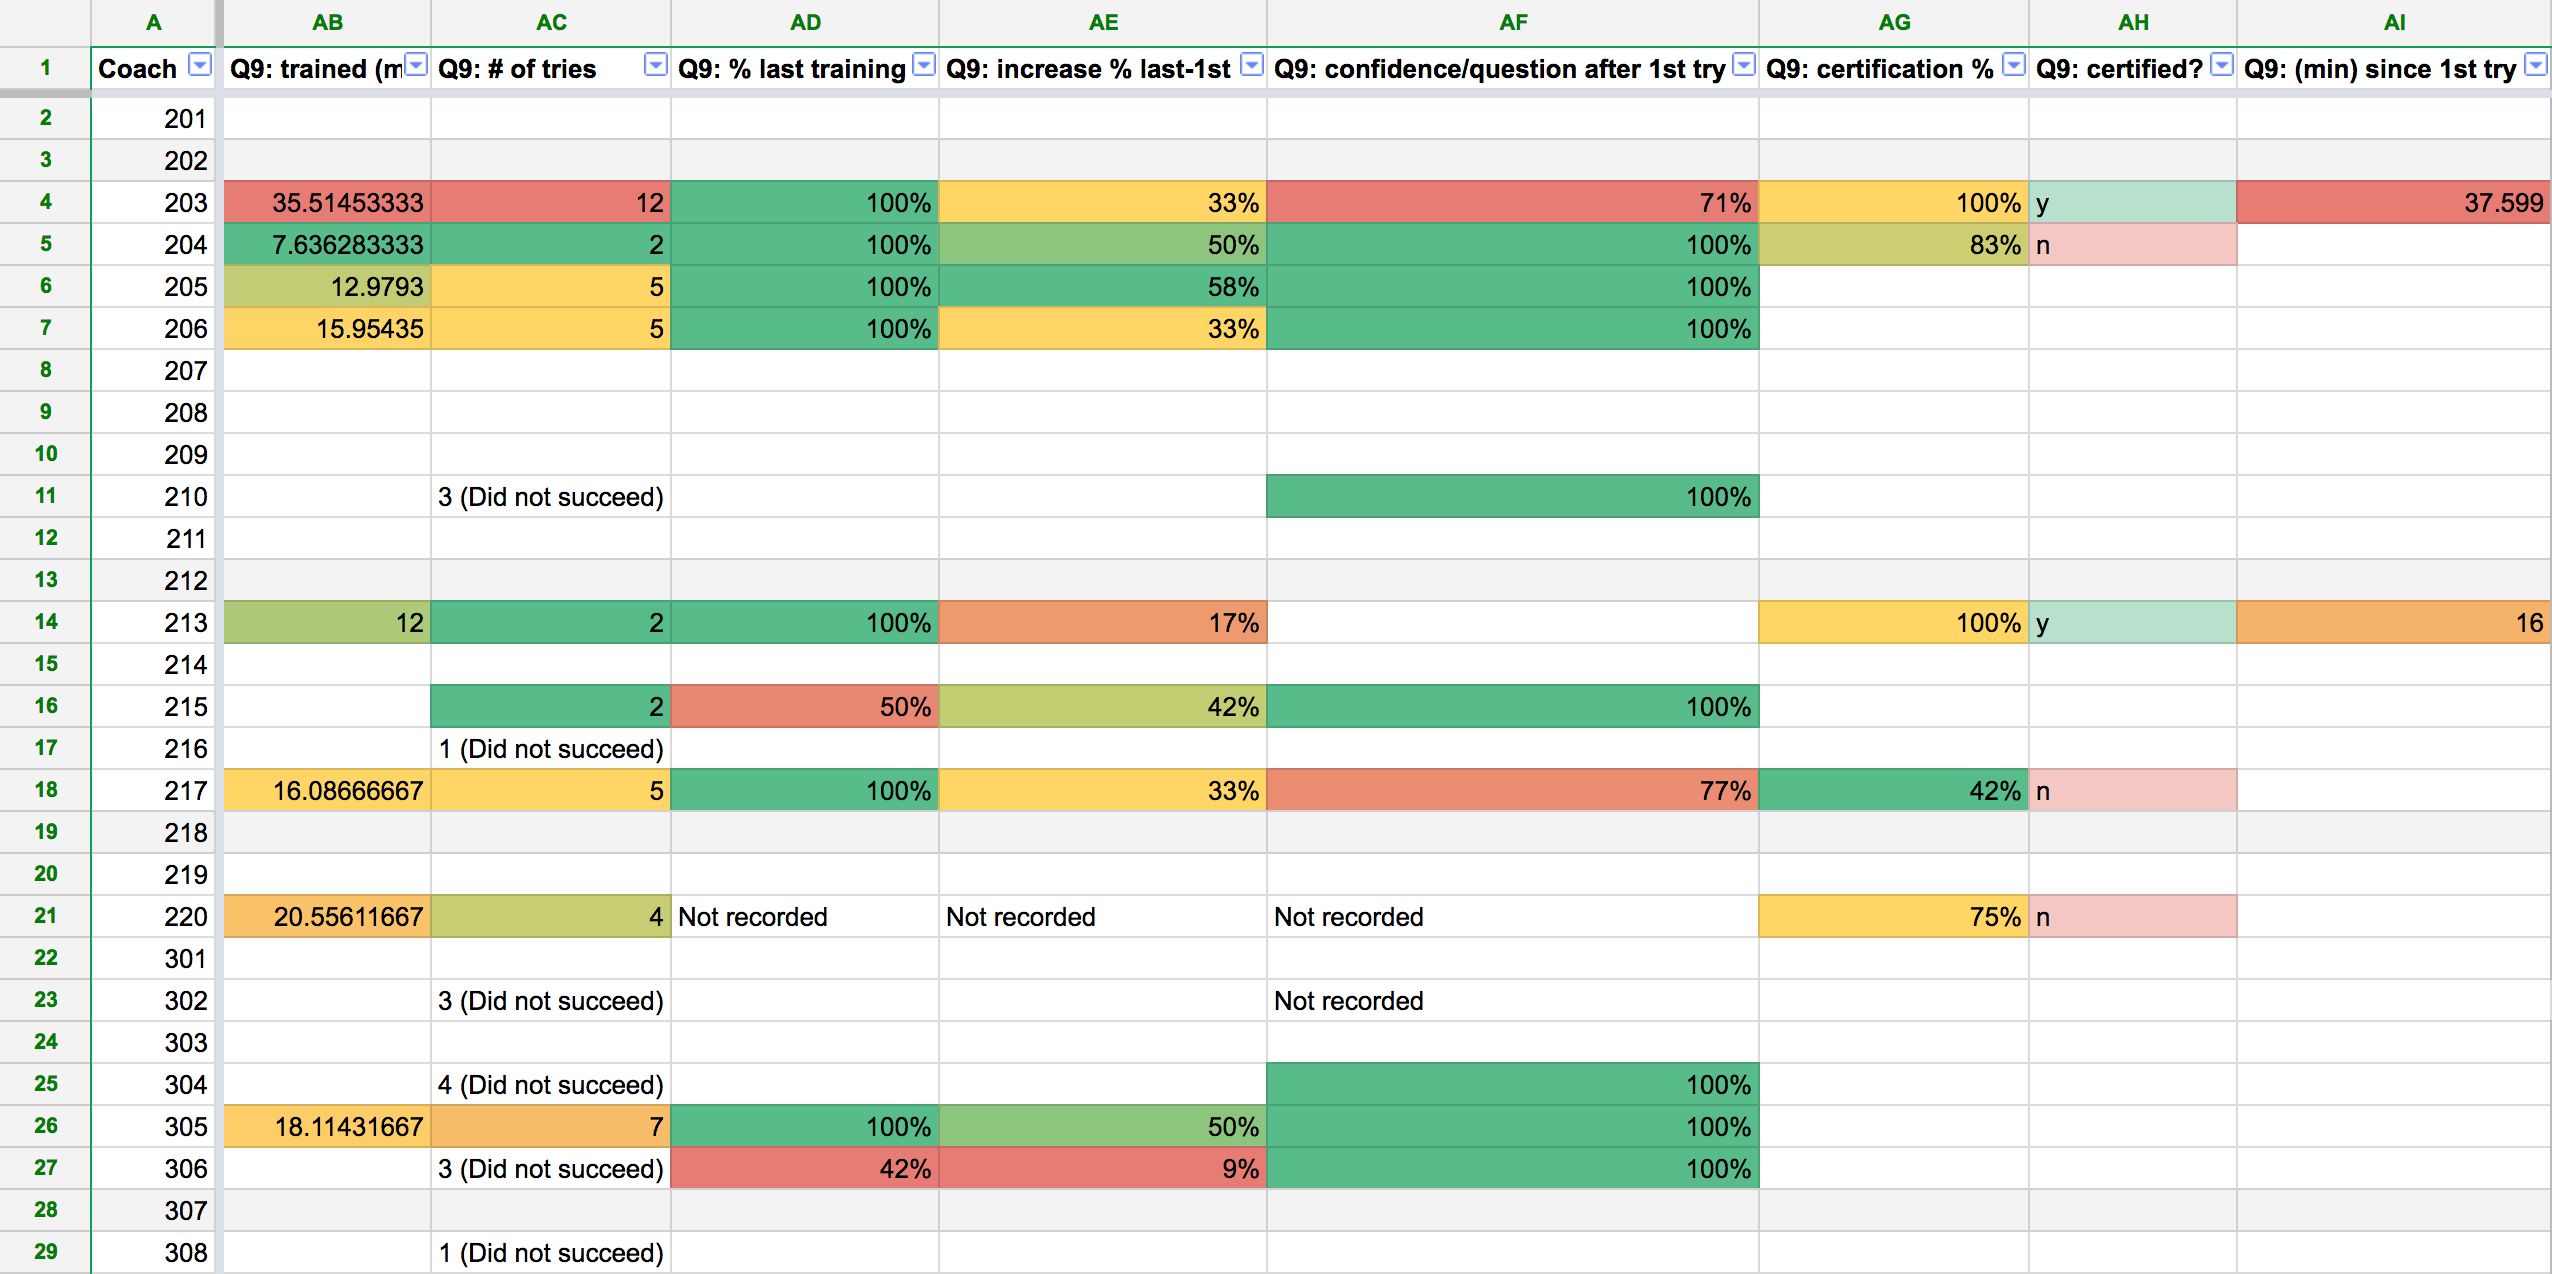
\includegraphics[width=1.0\textwidth]{analysis/sheets/3Quiz9B.png}
    \caption{Quiz results on the training and certification of coach guide quiz 9 "Are you ready?". Column AB: how many minutes they spent in training. AC: how many times they pressed "Try again", retaking the wrong answers. AD: their score on the last training quiz they took. AE: the increase from their first training to their last. AF: recorded "Are you sure?": "Yes/No" after taking the quiz try 1. Finally, for the coaches that started the certification, their results are shown, together with the time the quiz took for those that got 100\% correct on the first try.}
    \label{fig:3Quiz9B}
\end{figure}

\begin{figure}[h]
    \centering
    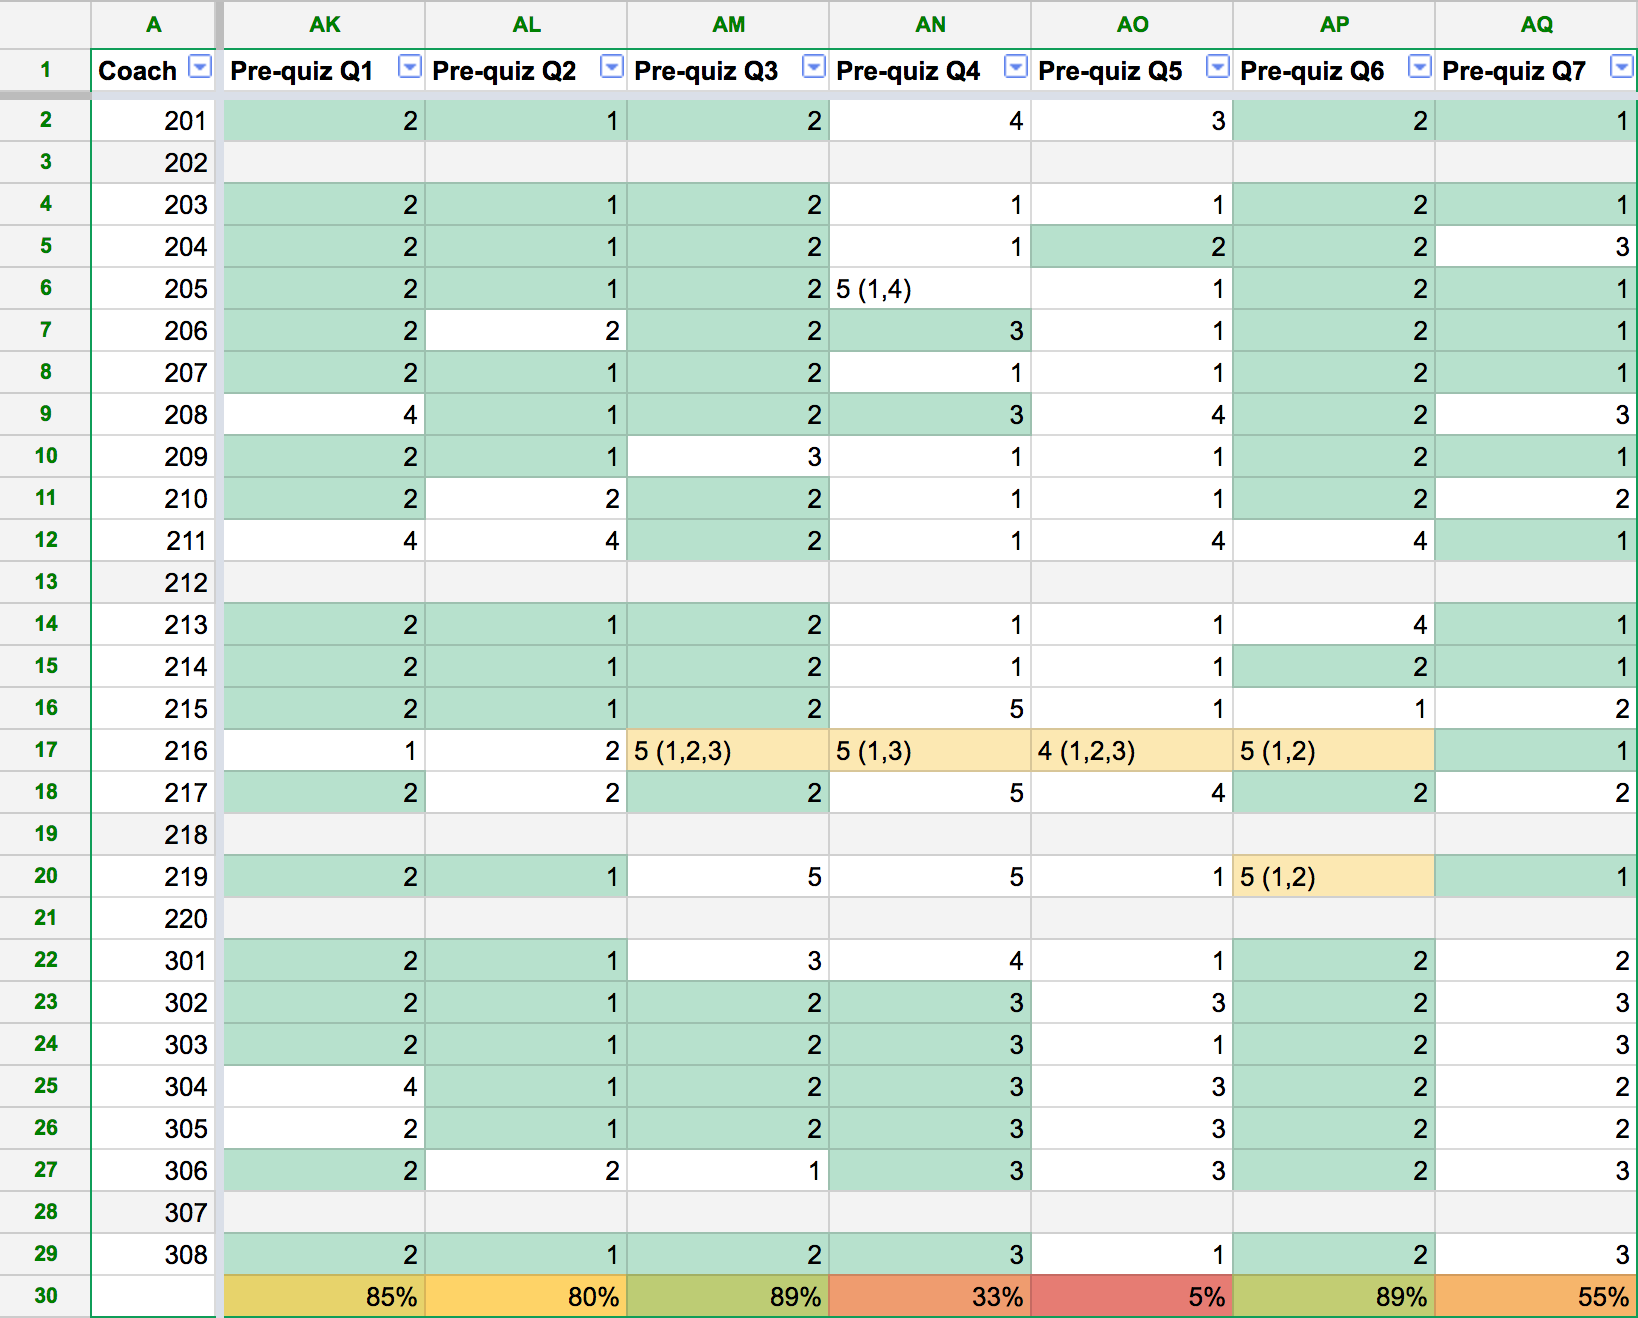
\includegraphics[width=1.0\textwidth]{analysis/sheets/4Pretest.png}
    \caption{Pre-quiz results per question and coach. The correct answers are given in green. The questions asked can be observed in Appendix \ref{cha:pre-test}}.
    \label{fig:4Pretest}
\end{figure}

\clearpage

Missing cells was not as obvious with the app results, were users could not progress in a quiz without answering both the question and the confidence. However, none of the passed quiz 9 certification answers had been submitted. Thus, it was needed to add these from the manual recordings, which had been used as a backup in case anything like this would happen.

There were a number of quick insights that could be drawn before the parallel coordinates visualization, simply by looking at the data as a spreadsheet.

It was believed that smartphone users feeling like novices might have a disadvantage with the app, since they will not learn as fast as experienced users. The interactions shows however, between iteration 3 to 4, almost all of the coaches does not feel intermediate instead of beginners using the smartphone and the YoungDrive app. The quiz data verifies this, with no direct correlation between technical skills and quiz results (comparing column H "Smartphone level" 1-3) with column M and T (quiz scores on the first try for quiz 3 and 9). From the pre-test data, it can be seen that only CBTs said they didn't feel comfortable with smartphone (n=2, column H, of which there were 6 Youth Mentors and 14 CBTs). A reason might be age, as CBTs were older than the Youth Mentors. Also, youth mentors had higher school level than the CBTs. More probable, is that the experience of using a smartphone since iteration 3 has matured over time, and that they are now more confident. %It is interesting that this has improved since iteration 3, possibly indicating that the smartphone skills have matured since the last test two weeks ago.

From the Google Sheets quiz results data, it could be seen that there was a surprisingly low number of answers where the user answered the question without confidence (see column P, U and AF). This is not good for feedback purposes, as answers were actually often not correct.

First-hand insights before the parallel coordinates were that there was a strong correlation between pre-quiz results (column D) and quiz 9 try 1 (column T), and slightly visible also in quiz 3 try 1 (column M), but with more outliers. Also, with manuals there was a higher probability of finishing quiz 9 training and certification (see also findings from the parallel coordinates visualization below). The data shows small tendencies that being honest and deliberate during the training increases the likelihood that a coach can get 100\% without faults, and has truly learned.

The final version of the app shows users can get 100\% on quiz results much faster (column R, AB and AI) than the previous version, as the score board had been improved for iteration 4. Since the target group in Zambia and Uganda was different, it is hard to empirically prove if it went faster getting 100\% with the possibility of repeating only the wrong questions, asking "Are you sure?", and providing individual feedback. Asking after the app does in iteration 4 does show however, that 100\% of the coaches now thought the feedback was good for learning.

%\subsubsection{Bonus Result: Learnings from Observing All of the Quiz Results}
Also, from observing all of the quiz submissions (see sample in figure \ref{fig:unprocessedData}), more users had started a quiz without finishing it than anticipated. This speaks for usability issues (cancelling the quiz by mistake, like clicking the back button, or loss of internet access) or bad technical skills (needs to design to be more fail-safe) or lack of motivation (needs to design for unmotivated coaches as well. The need group of "challenged coaches" might need other design than "ideal coaches".

Finally, a lot of users had done quizzes that were not Topic quiz 3 and Coach quiz 9, which might indicate high interest (if they did more than 2 quizzes) or confusion (if they did not do 3 or 9, but they did do other quizzes) during the app evaluation. This meant that on some aspects, there were less data than anticipated, (which was troublesome, as there were already few data points), and some aspects where there was more data than anticipated (on overlooked other quizzes).

\subsubsection{Parallel Coordinates Visualization}
Statistical analysis in R showed that none of the results were statistically significant to be notable using linear regression, or any of the other statistical methods detailed in the methodical framework. It was believed that statistical analysis could at least give insight into what to look for in the parallel coordinates visualization, but also for this, a larger sample would be needed. An interactive parallel coordinates visualization could give many more insights, more faster than the static presentations in Google Sheets or statistical analysis in R.

There is an almost infinite number of findings and observations that are interesting to look at via the parallel coordinates visualization. Even if there are no clear correlations (which are often found immediately when working with large data sets and parallel coordinates), tendencies can be found. As nothing is statistically significant (mostly because of the small data sample), the only thing that could be found are tendencies, and to analyze outliers. Then, these findings was critically analyzed to characteristics, and observations made from the app tests. As such, the data should be seen as indications of where future research is interested, and not as universal truths. For further research into the data, see figure \ref{fig:parallellCoordinates3} and the below sections.

\begin{figure}[h]
    \centering
    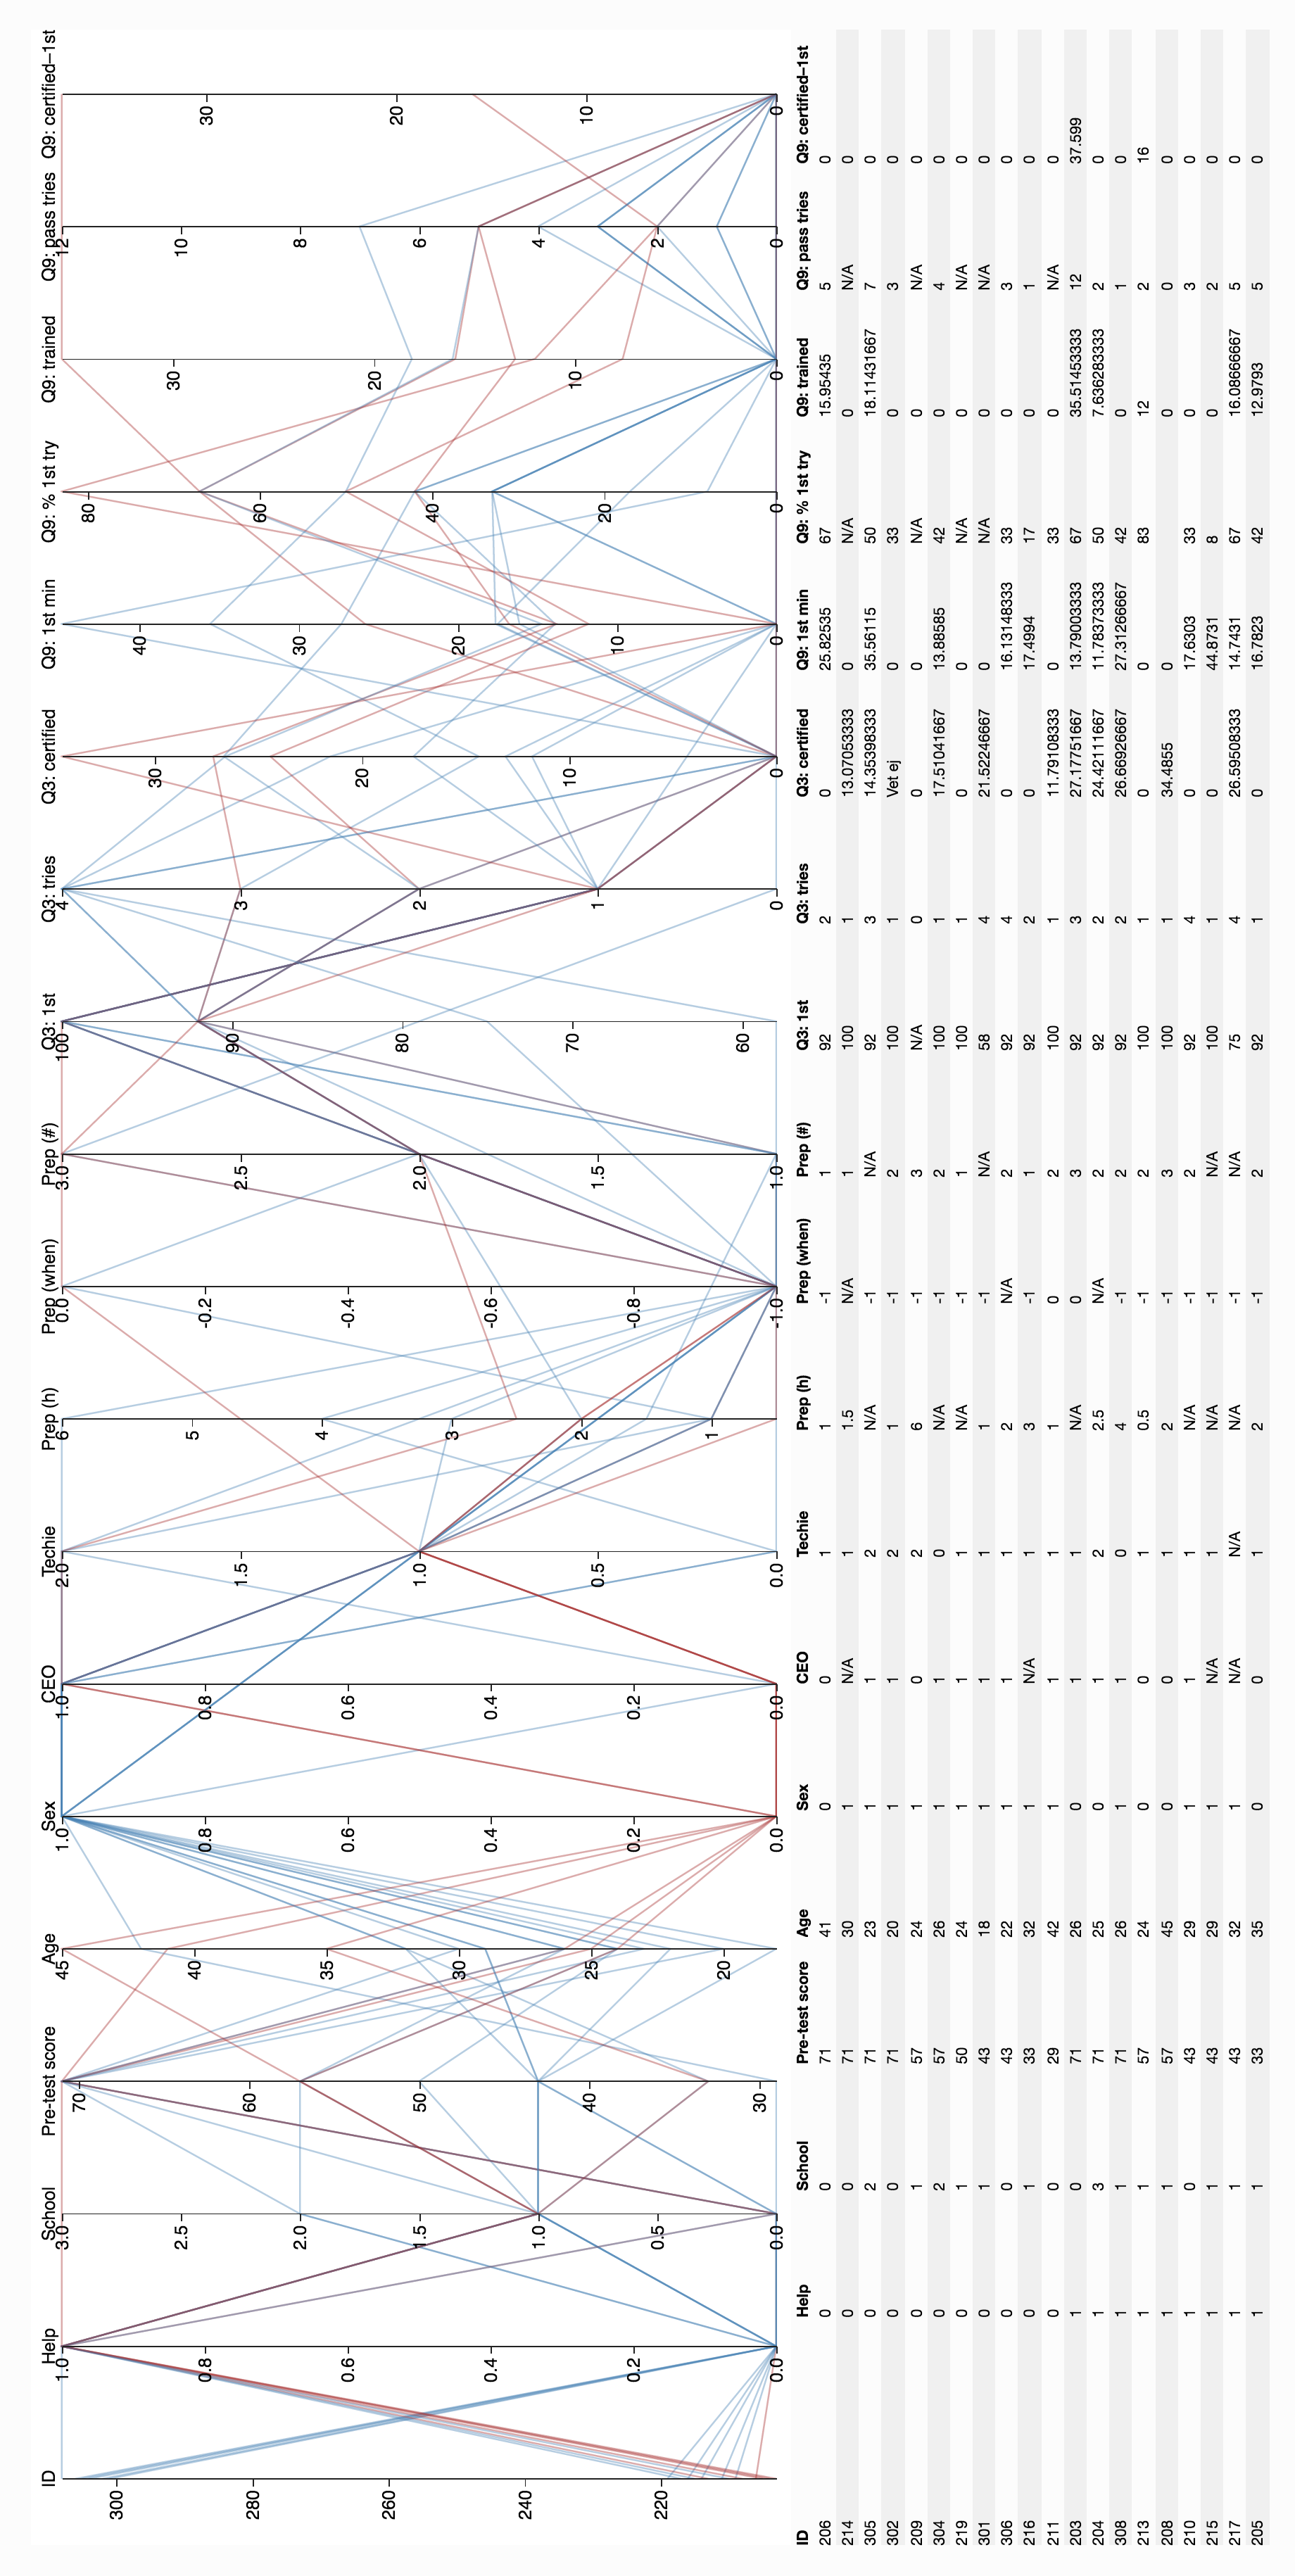
\includegraphics[width=0.7\textwidth]{analysis/parallellCoordinates3.png}
    \caption{The quiz results from iteration 4 shown in an interactive parallel coordinates visualization. The visualization is available on \url{http://marcusnygren.github.io/youngdrive-parallel-coordinates/}.}
    \label{fig:parallellCoordinates3}
\end{figure}

\clearpage

%* 1/6 Youth mentors had brought manual, compared with 8/14 CBTs
%* There are no female Youth Mentors (i.e. 100\% male Youth Mentors)
%* All of the YM's run their own businesses, compared with 5/10 for CBTs

%* Seemingly no difference CBT vs. YM in when prepares for session
%* All YM prepares 2 times for session, while CBT can train also 3 or 1 time)

%* 13/14 CBTs gjorde quiz 3 try 1, 6/6 YM's
Following the lines from column "ID" (for Coach ID), you can compare the difference in performance between Youth Mentors (301-308) and CBTs (201-220). Between quiz 3 and 9, there is no unison difference. In quiz 9 however, the Youth Mentors are top performers compared to CBTs, which goes in line with the project leaders opinion in the field that Youth Mentors are slightly better in the field than the CBTs. This could be explained also by that Youth Mentors only teach YoungDrive, while the CBTs also teaches other programs. It is important to note that there is nothing statistically significant to draw confident conclusions. Further research needs to be made, as a connection between how a coach performs in the field versus the app is valuable. %CBT 6/14 st certifierade, YM 4/6 st

%Quiz 9 (rött=CBT:
%* 6 CBTs gör ej Q9 try 1, 2 YM gör ej
%* YM är top performers på Q9 try 1 jämfört med CBTs
%* endast 1 YM klarade däremot träningen, medan
%* YM's är bättre på quiz 9 try 1 än CBTs
%* Det är endast 1/7 som klarade quiz 9 training som är Youth Mentor
%* Antal försök man gjorde är likvärdigt, förutom en YM som hade 12 försök (och klarade quiz)

%If the app is indeed an indicator if the coach performs well, the data shows that female coaches should be hired for YoungDrive.

The results shows that the ideal coach, according to the quiz app, would be a woman, both in contrast and in unison with the literature mentioned in section \ref{entrepreneurship-education}. In figure \ref{fig:parallellCoordinates3} it can be seen that the female coaches (red lines) on average has better scores than the male coaches (blue lines), in spite of having less formal education. Further, she prepares more, is more aware of her own knowledge and has a better study technique, respecting the app feedback for meta-cognition and meta-memory. More than average, for example in quiz 9, the women have a higher lowest threshold, and a much higher record, than the men. two people were fast enough to get certified on the final quiz before the app evaluation ended, see figure \ref{fig:quiz9pl}. Both were women. Apart from gender, these coaches had higher quiz results, faster learning, and more honesty in "Are you sure?" than the others. Today, the balance between male and female coaches is reversed from what the data says: in Zambia only men have been hired, and in the data collection for Uganda, only 30\% (6/14) were women.

%\textbf{Certified quiz 9}
Other social characteristics on the two coaches that passed the certification for coach quiz 9 is that were that both were CBTs (not youth mentors), and were in the middle of the age groups (24 and 26 years old). Regarding performance, they had a good pre-test score (57\% or 71\%), had top scores on quiz 3 try 1 and 9 try 1. Also, both of them used the manual, they looked at themselves as medium-skilled using a smartphone, and they prepared many times per youth session (2 or 3 times). In figure \ref{fig:quiz9pl}, a more detailed explanation is given. What didn't seem to matter for top performance, was number of tries for passing the training of quiz 9 (one coach did 2 tries on quiz 9, the other 12 tries), or time to pass training quiz 9 (35.5 minutes on the slowest versus 12 minutes on the fastest). Neither did it seem to matter when they prepared their session (1 did preparations the same day, 1 the day before). Regarding social characteristics, one had a business, one didn't, and their school level were both low.

\begin{figure}[h]
    \centering
    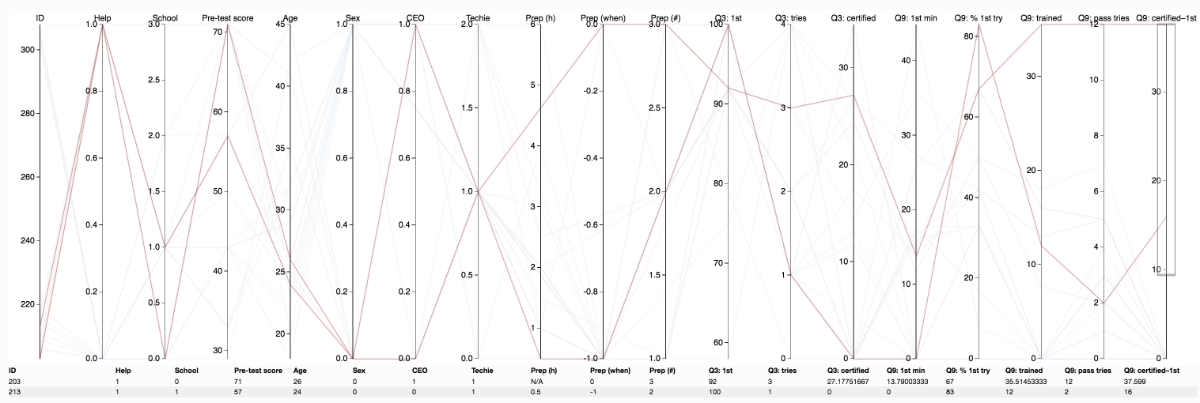
\includegraphics[width=1.0\textwidth]{analysis/paralellCoordinatesWomen.png}
    \caption{The parallel coordinates visualization showing the characteristics of the two coaches that passed the quiz 9 certification. They were both CBTs, they could both could consult the manuals, they had a low education, while still having higher pre-test scores that the average. They were relatively young and were both women (in minority). One had a company and one did not. The one that inserted how she prepared for session, said she prepared the day before (versus doing it the same day), on three occations. Regarding quiz results, they both had a high score on try 1 of quiz 3 "Financial literacy" (1 or 0 errors), just like the majority, and it took them 1 or 3 tries to pass the training. For the coach where time is recorded for getting certified, it took her 27 minutes to pass the quiz (higher than the average). On quiz 9, it took 13 minutes to get 67\%, the other coach (time not known) scoring 83\%. While the coach with 83\% passed the training in only 12 minutes and 2 tries, it was the coach taking 35 minutes to take 12 tries that could afterwards get all of the answers correct in the Certification.}
    \label{fig:quiz9pl}
\end{figure}

Finally, it is interesting to observe the differences (and lack thereof) between the test group and reference group, by following the lines from the second column, "Help", of figure \ref{fig:parallellCoordinates3}. In the test group ("Help" = 1), the paper manuals could be read before improving on the quiz results (not during the actual test) The the reference group ("Help" = 0) were only allowed to observe the right answers within the app, from the score board. In quiz 3, where almost all coaches had 92\% or 100\% immediately, there is no difference observable. However, in quiz 9, the hardest quiz, 5/7 that passed the training were in control group A, and 2/2 that passed the certification were in control group A. An explanation could be that the large amount of questions made the correct answers hard to memorize versus actually learning, or that the ones with manuals felt more supported or motivated because of the extra support. While these findings could be true for a larger sample, further research needs to be done. The same methods of data analysis are increasingly relevant with a larger data set, and there seems to be correlations and tendencies worth looking further into.


\subsection{Analysis of Interviews}

The answers given during the three group interviews has been summarized and clustered into three areas, see figure \ref{fig:overview}. Further, the answers within interaction design has been clustered into its four main principles, see figure \ref{fig:interactiondesign}. The questions regarding learning has tried to answer why a coach is correct or incorrect on a given question, see figure \ref{fig:learning}. Service design has been clustered into the two questions "When do you want to use the app?" and "When are you not able to use the app?", see figure \ref{fig:servicedesign}. Zoomed-in versions of all of the areas are presented after the overviews, where the analysis of the quotes can be seen in its fullest. The quotes from these mind-maps are individual, which means that if another coach has had a similar thought, their quote is branched next to the following quote.

\begin{figure}[h]
    \centering
    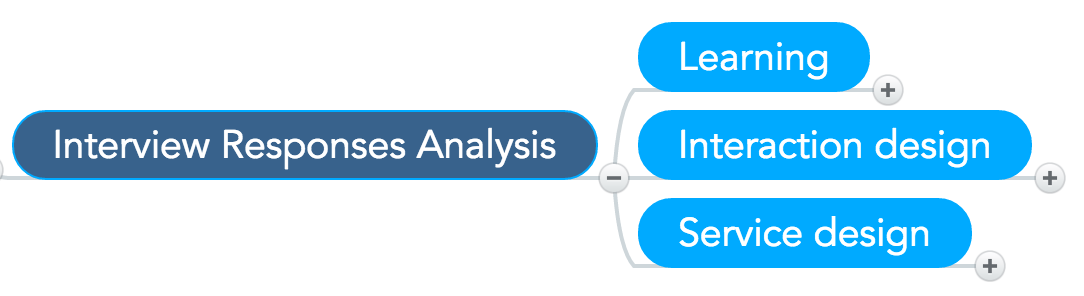
\includegraphics[width=0.3\textwidth]{analysis/interviews/overview_notexpanded.png}
    \caption{The interview answers has been clustered into three areas: learning, interaction design and service design.}
    \label{fig:overview}
\end{figure}

\begin{figure}[h]
    \centering
    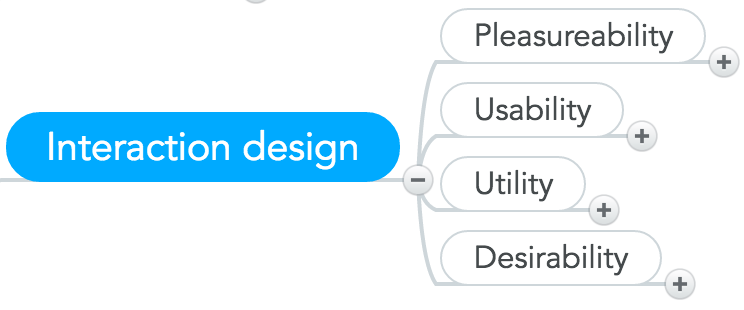
\includegraphics[width=0.3\textwidth]{analysis/interviews/interactiondesign_notexpanded.png}
    \caption{The coach quotes regarding interaction design has been divided by four criteria: pleasurability, usability, utility and desirability.}
    \label{fig:interactiondesign}
\end{figure}

%For learning and service design, the analysis of the interview quotes can bee seen in its fullest in figure \ref{fig:learning} and figure \ref{fig:servicedesign} respectively. Zoomed-in versions of all of the areas are presented after the overviews, where the analysis of the quotes can be seen in its fullest.

\begin{figure}[h]
    \centering
    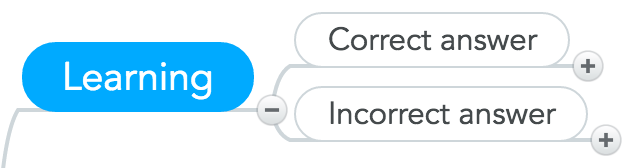
\includegraphics[width=0.3\textwidth]{analysis/interviews/learning_notexpanded.png}
    \caption{The coach quotes regarding learning has been divided by if they give insight to why a coach has been correct or incorrect on a given question.}
    \label{fig:learning}
\end{figure}

\begin{figure}[h]
    \centering
    
\includegraphics[width=0.3\textwidth]{analysis/interviews/servicedesign_notexpanded.png}
    \caption{The coach quotes regarding service design has been divided into \textit{when} you want to use the YoungDrive app, and when you are hindered from doing so.}
    \label{fig:servicedesign}
\end{figure}

\clearpage

\subsubsection{Learning}\label{sec:interview-learning}

By reading the quotes from the coaches carefully, it can be understood why answers can appear correct by the coaches (see figure \ref{fig:learning1}), even if this would not be the case (see figure \ref{fig:learning2}.

\begin{figure}[h]
    \centering
    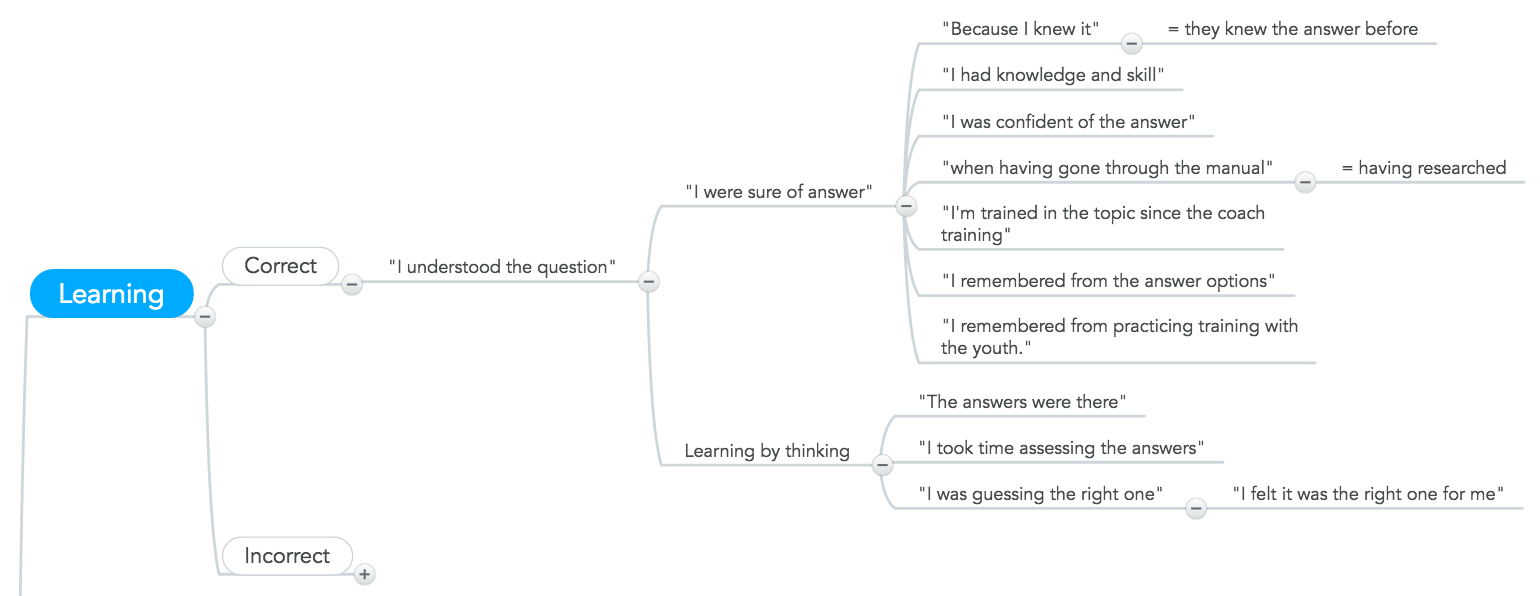
\includegraphics[width=1.0\textwidth]{analysis/interviews/learning_correct.png}
    \caption{Quotes explaining why a coach could give an correct answer on a given question. Either you were sure of the answers, or you made a qualified guess. A prerequisite for answering the question correct is that you understood the questions meaning.}
    \label{fig:learning1}
\end{figure}

\begin{figure}[h]
    \centering
    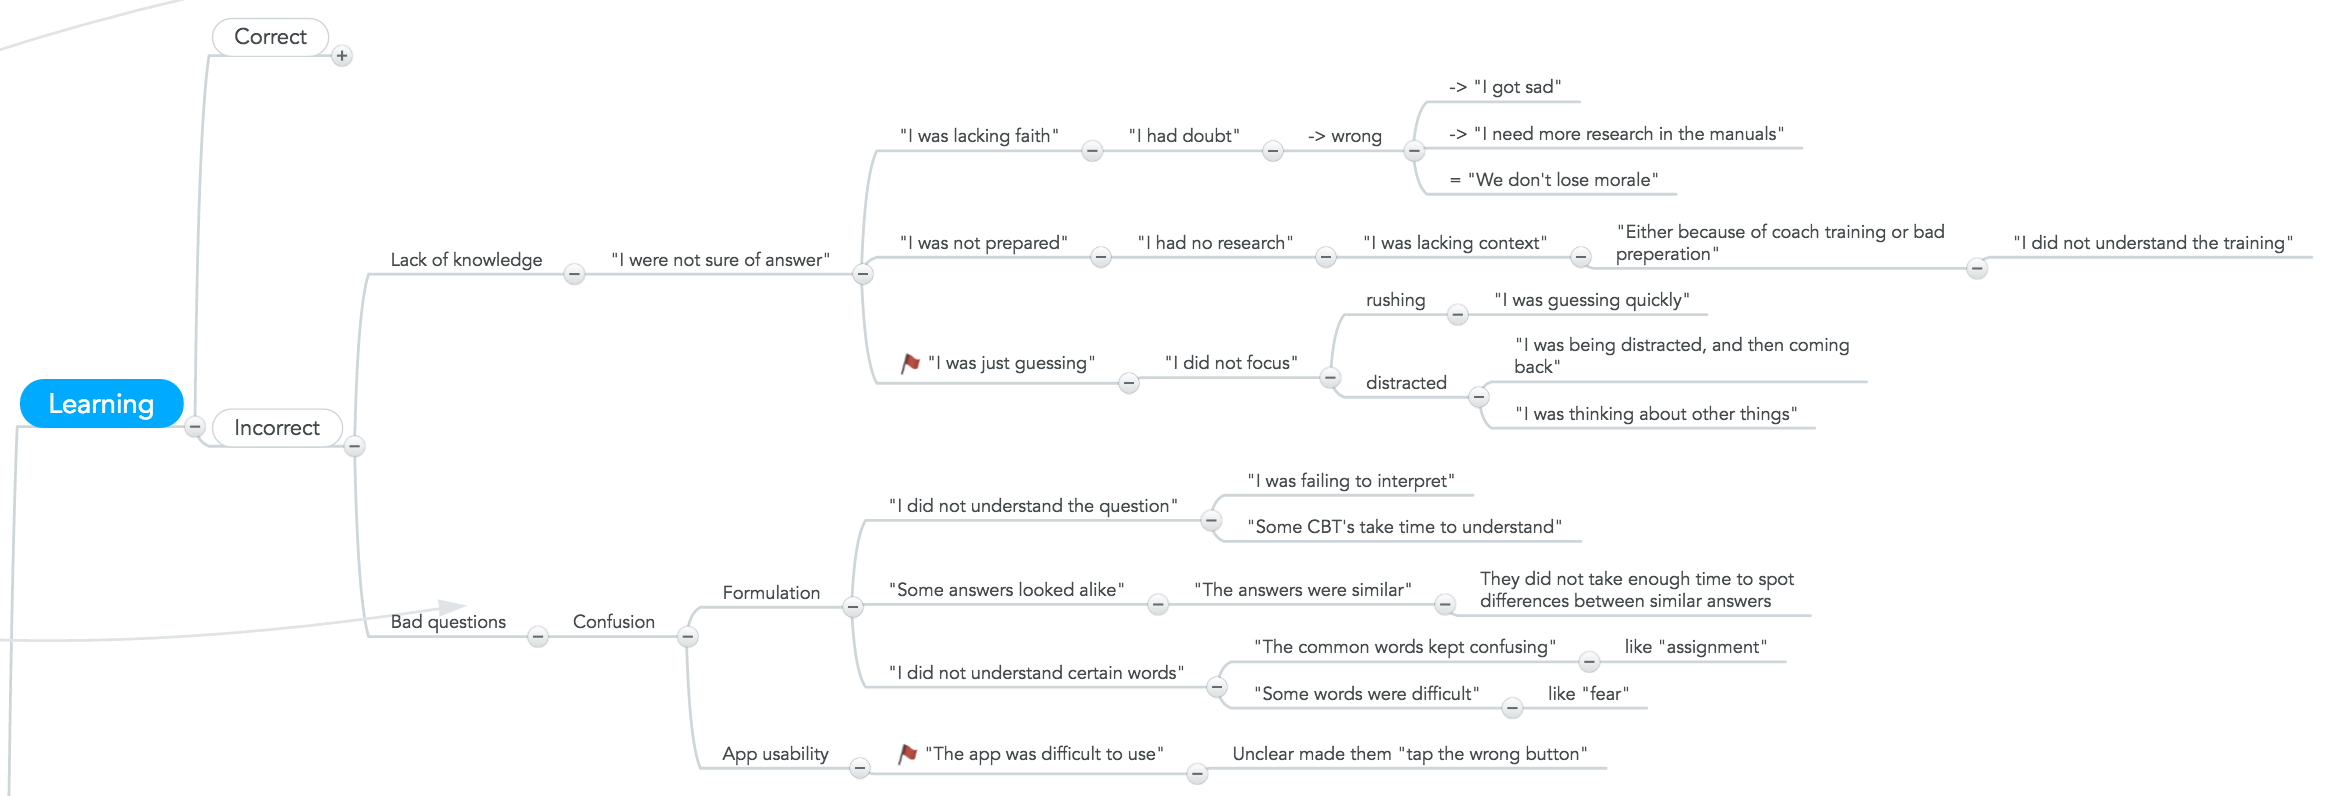
\includegraphics[width=1.0\textwidth]{analysis/interviews/learning_incorrect.png}
    \caption{Quotes explaining why a coach could give an incorrect answer on a given question. Either, the coach did not have sufficient knowledge to answer the question confidently (for a number of reasons, given in the figure), or the question was not understood correctly, or the app usability was a hindrance.}
    \label{fig:learning2}
\end{figure}

\clearpage

\subsubsection{Interaction Design}

Most importantly, in the final app test, everyone thought the app was good and easy to use (n = 26). This is important, as this had not been the case in iteration 3. Regarding the four different areas of interaction design, positive remarks on utility are especially beneficial for learning. However, pleasurability, usability and desirability is a prerequisite for the app to be used by the coaches. For desirability, if the coaches are stimulated by using the app, two reviews were: "It felt good using the app" and "It motivated learning". The other three interaction principles (pleasurability, usability and utility) have been given their own mind-map below, see figure \ref{fig:interaction1}, figure \ref{fig:interaction2} and \ref{fig:interaction3}.

\begin{figure}[h]
    \centering
    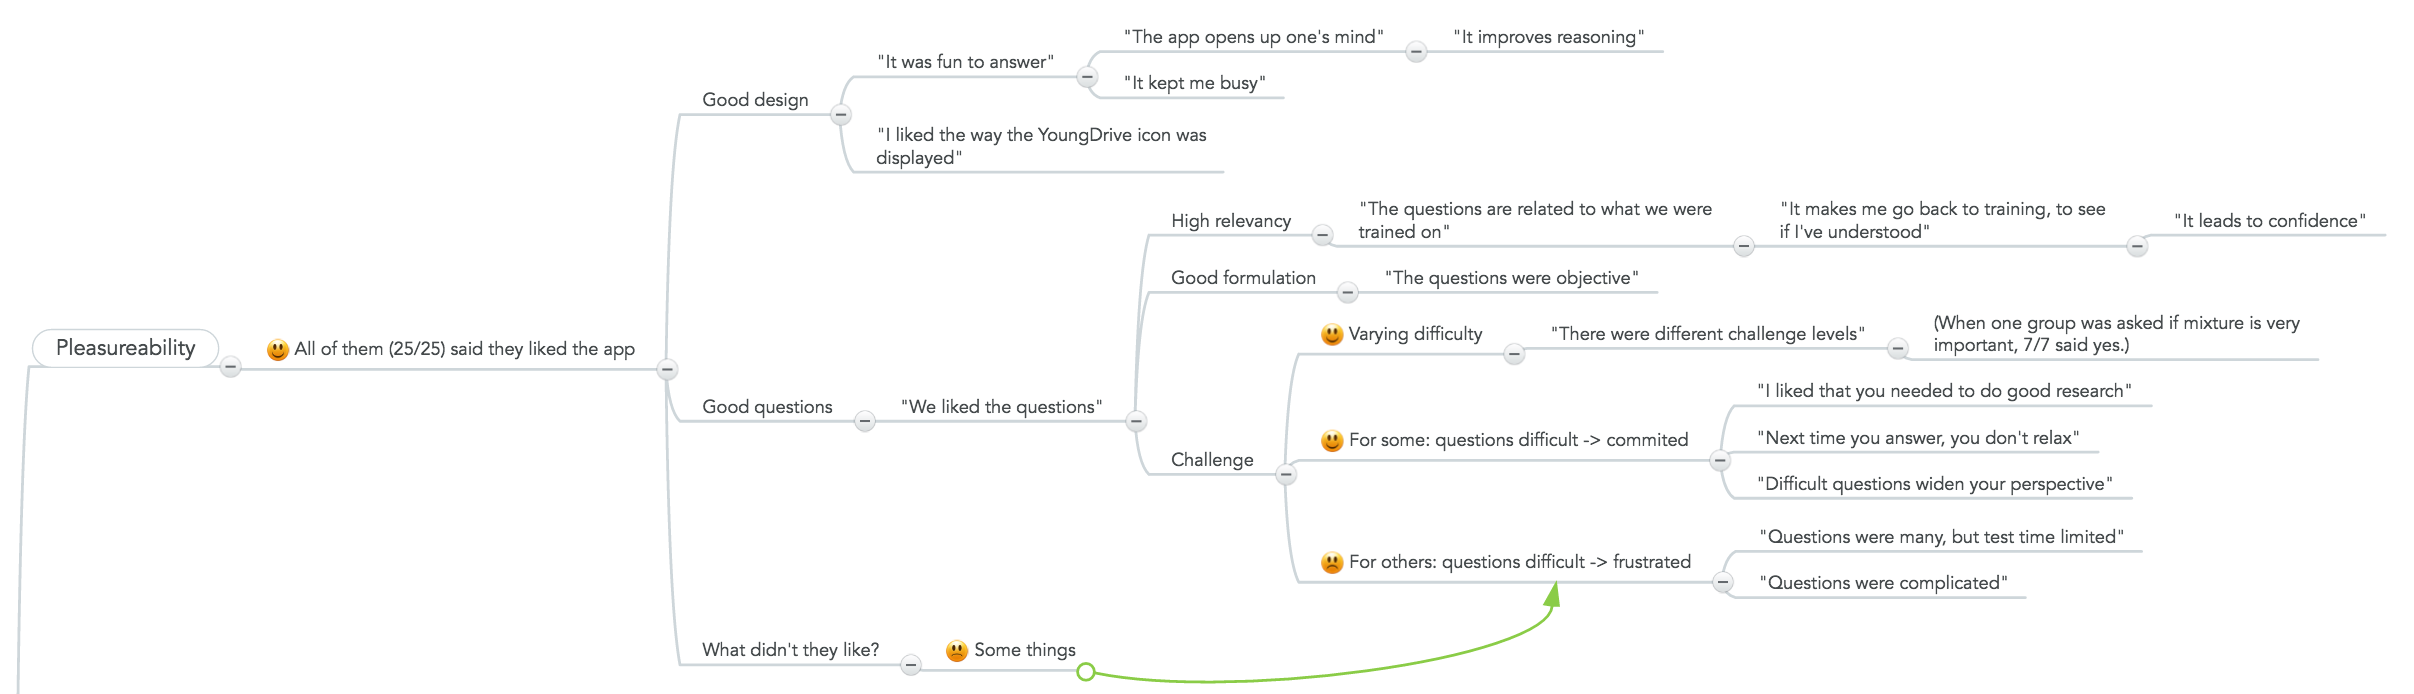
\includegraphics[width=1.0\textwidth]{analysis/interviews/interactiondesign_pleasurability.png}
    \caption{Pleasurability was 100\%, as the app had a good design and well-motivated questions, however some coaches were frustrated by difficult questions in the app, or the time needed to complete a quiz during the workshop.}
    %From the interviews, it is visible that the coaches feel the quizzes has been a fair way to measure their knowledge in the topic. The answer "It leads to confidence" could show that when a coach has done a quiz reaching certification, they do feel more confident about teaching the topic.
    %Positively, assessment of "Am I ready?" can happen already before the youth session, in the app.}
    \label{fig:interaction1}
\end{figure}

\begin{figure}[h]
    \centering
    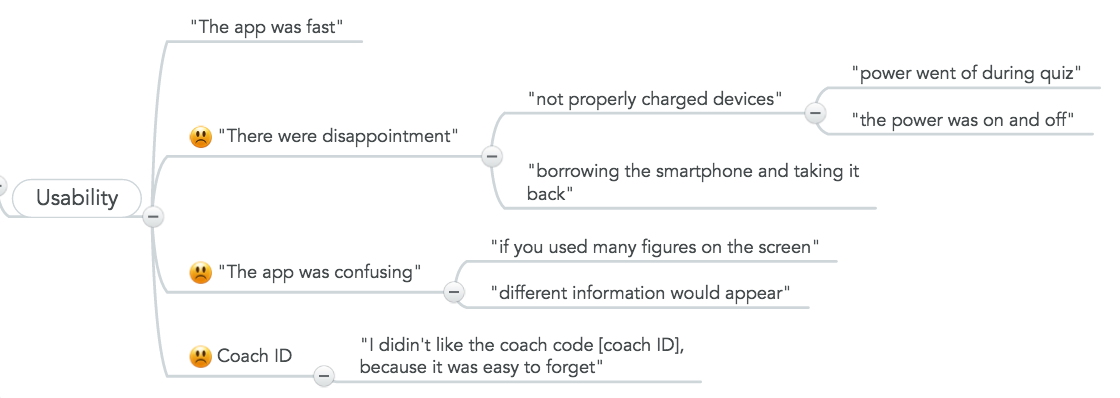
\includegraphics[width=1.0\textwidth]{analysis/interviews/interactiondesign_usability.png}
    \caption{Usability. As previosuly stated, all of the coaches (25/25) thought the app was easy to use when asked by raise of hands. However, in the interviews, some detailed comments regarding usability appeared. Regarding workshop issues, some of the devices' battery died during the workshop, or needed to be replaced. Regarding the app, some still mention too much information to appear at once, or that information are shown that the coach does not expect. Only one coach mentioned thinking that thee login was not user friendly, since the Coach ID was easy to forget. The Coach ID has since been documented by the local project leaders, so they can be contacted in such situations.}
    \label{fig:interaction2}
\end{figure}

\begin{figure}[h]
    \centering
    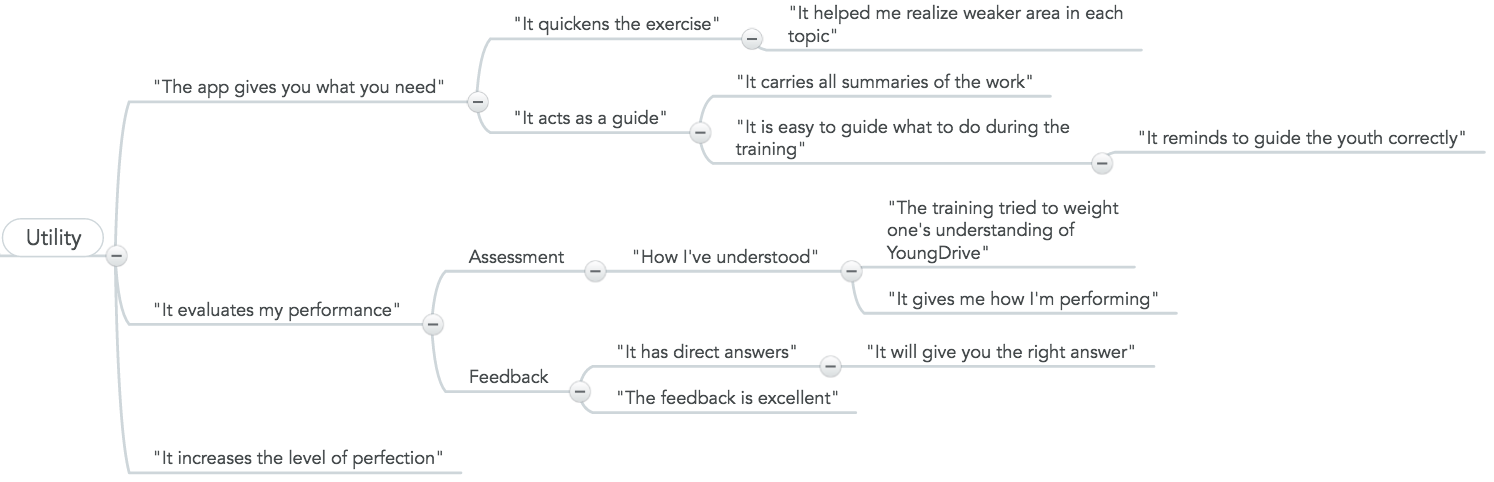
\includegraphics[width=1.0\textwidth]{analysis/interviews/interactiondesign_utility.png}
    \caption{Utility gives a valuable measure of what benefits the coach finds with using the app. Quotes regarding usefulness are: "It quickens the exercise", "It carries all summaries of the work", "It reminds to guide the youth correctly". For training, coaches conclude that "It evaluates my performance" and that "The feedback is excellent". One coach summarizes with "It increases the level of perfection".}
    \label{fig:interaction3}
\end{figure}

\clearpage

\subsubsection{Service Design}

It is important to understand if and when the app will be used by the coach, and if the environment of the coach in any way can hinder use of the app. For understanding the coach situation to these two criteria, see figure \ref{fig:servicedesign1} and \ref{fig:servicedesign1}.

\begin{figure}[h]
    \centering
    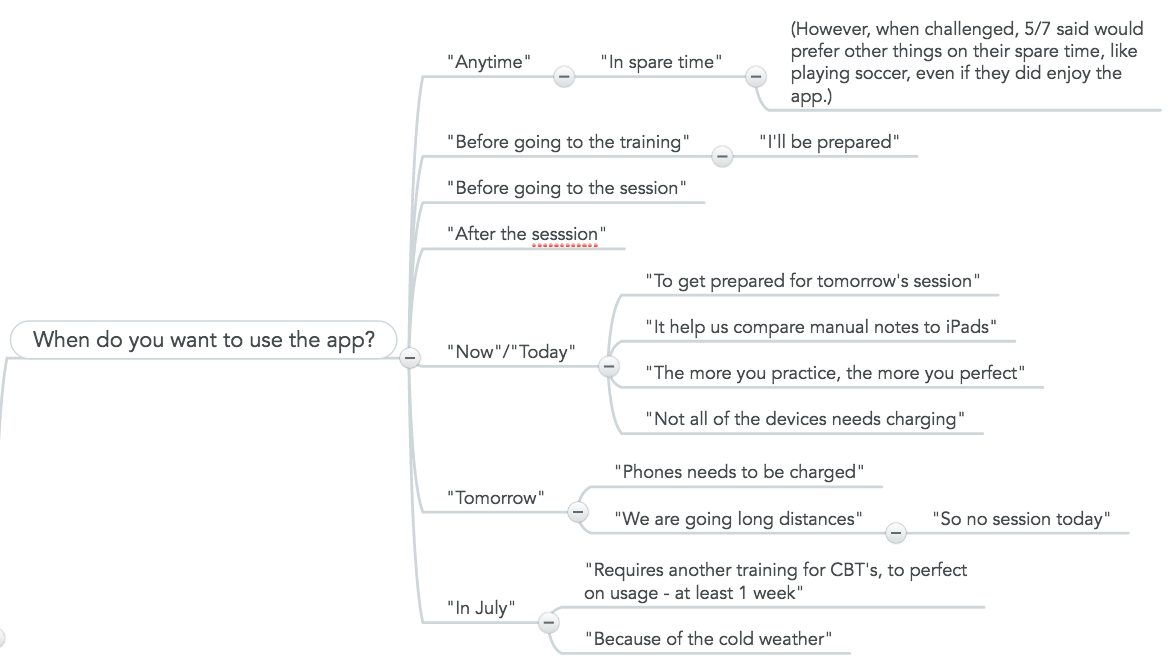
\includegraphics[width=1.0\textwidth]{analysis/interviews/servicedesign_when.png}
    \caption{There are very varying answers to the question "When do you want to use the app?". Most coaches would have liked to use the app immediately. Some of the coaches identified the need for devices, more training, or charging of devices in being able to do so.}
    \label{fig:servicedesign1}
\end{figure}

\begin{figure}[h]
    \centering
    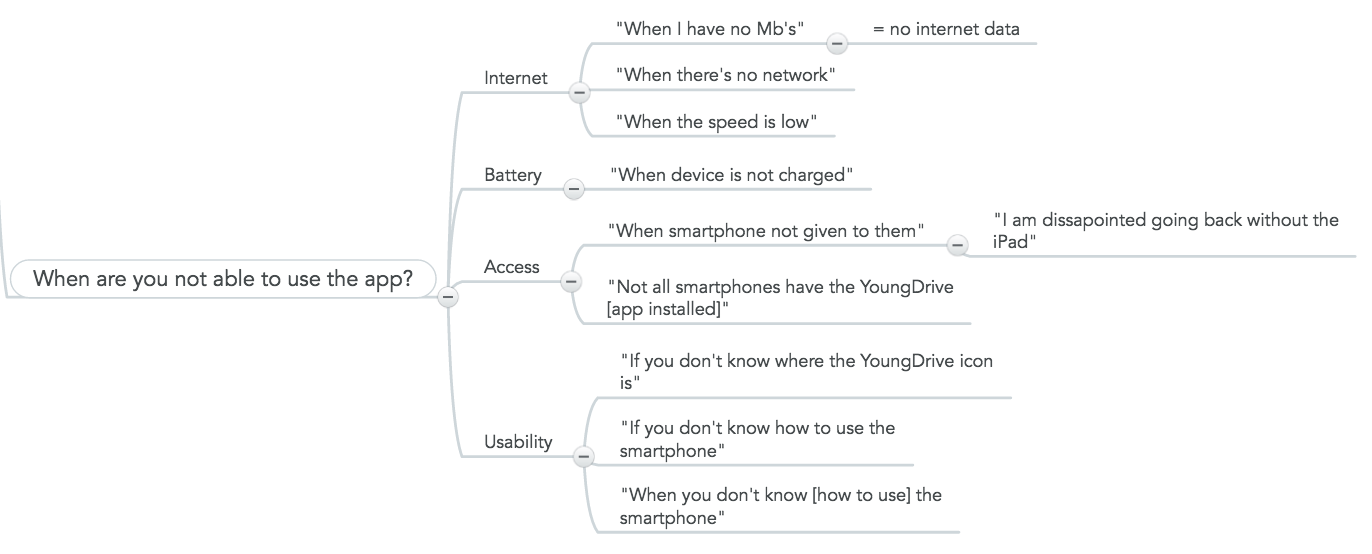
\includegraphics[width=1.0\textwidth]{analysis/interviews/servicedesign_cant.png}
    \caption{Answers for the question "When are you not able to use the app?" are grouped into four segments: internet issues, battery issues, low or no access to smartphones, or if the app is not usable because it is not available on the smartphone, or the coach does not know how to use a smartphone.}
    \label{fig:servicedesign2}
\end{figure}

\clearpage

%\subsection{Conclusions}

\todo{Add everything from the mindmap}

In three months time, an app was developed with precision to the needs and context of the end users. The design has been heavily influenced by the end users, from day 1 of the project, in conjunction with relevant research, and in balance to stakeholder goals and considerations, and supervisor advice.

The results shows that the ideal coach, according to the quiz app, would be a woman, since she has better knowledge in spite of having less formal education. She prepares more, is more aware of her own knowledge and has a better study technique, respecting the app feedback for meta-cognition and meta-memory. This can be seen by higher quiz results, faster learning, and more honesty in "Are you sure?".

It could be that first-time smartphone users have a disadvantage with the app, since they will not learn as fast as experienced users. The interactions shows however, that at the second session, almost all of the coaches felt intermediate instead of beginners, using the smartphone and the YoungDrive app. The quiz data verifies this, with no direct correlation between technical skills and quiz results.

The final version of the app shows users can get 100\% on quiz results much faster that the previous version, where the score board had been improved. Since the target group in Zambia and Uganda was different, it is hard to say if it went faster getting 100\% with the possibility of repeating only the wrong questions, asking "Are you sure?", and providing individual feedback. The qualitative study does show however, that 100\% thought the feedback was good for learning, and that they appreciate the app.

The data shows that being honest and deliberate during the training increases the likelihood that a coach can get 100\% without faults, and has truly learned. Further, when a coach has passed the certificaiton, they do feel more confident about teaching the topic, since assessment of "Am I ready?" can happen already before the session, and they feel the quiz has been a fair way to measure their knowledge in the topic.


%For Discussion, Conclusion and Future Work, see the coming chapters.

%\section{Qualitative Data}
%
%  Here the results from the qualitative data for iteration 1, 2, %3 and 4 are shown.
%
%  \subsection{Qualitative data}

\subsubsection{Entrepreneurship education considerations}
Throught early interviews with YoungDrive staff, it is clear that YoungDrive's entrepreneurship education methodology goes hand in hand with the presented theory. It's mottos are: "Dream big, start small", "Learning by doing" and "We have fun!" \citep{youngdrive}.

Both in regards to designing for the users and for the above reason, the app should be a complement to YoundDrive's existing training material and the structure of the program.

A challenging part of the work is that YoungDrive consists of both the practical skills of the entrepreneur, theoretical material of running a business, and an entrepreneurial mindset. Therefore, both how to assess knowledge, and build habits, needs to be examined.

\subsubsection{Understanding the coach situation}

A CBT can be responsible for from 7 up to 12 different youth groups in different programs, and such a high number places huge demands on the CBT.

Even if there are only 7 groups, being behind on schedule or not being confident, can be very demanding.

\textbf{Stayover at Patrick:} På morgonen visade Patrick mig hur han jobbar med deras tomt, var det odlas ris, och andra råvaror, deras djur, deras story från Syd-Sudan, till Kampala, till hyddan här i Tororo, och hans värderingar.

Efter en ungdomssession nästföljande dag besökte vi och hälsade kort på en av de 2 CBT:s vi har session med idag. Sedan hade jag och Patrick den obligatoriska review av ungdoms-sessionen, och jag bjöd honom på middag. Kl. 19 ringde hans fru (som har börjat få tecken av malaria) och skyndade hem.

Nästa ungdomssession fick jag besöka en annan CBT. Vi var tidiga. Sedan började jag prata med henne, och fick bra tillfälle att intervjua henne och även förklara för henne vad jag gjorde där. Det blev underligt att förklara för henne: Patrick påminde, när jag tabbat mig, att “Marcus, du måste förklara för X vad en app är”. Så hon fick låna min mobil, och jag förklarade att app var kort för applikation, och att för varje applikation har ett eget syfte, t.ex. ta foton. Jag bad henne klicka, svårt, råkade klicka åt henne, men sedan lät jag henne göra. Efter hon sett att det hon såg i skärmen var det hon såg på riktigt, blev hon jätteglad och började fundera vad hon skulle fota. Hon reste sig och gick runt hörnet, och jag följde efter. Hon fotade, efter att noggrannt tänkt igenom, att hon fotade buskarna med frukt. Sedan sade jag hon kunde fortsätta fota, och då tog hon ett litet runt hus utanför.


\subsubsection{Different kind of coaches}

The interviews with CBTs, PLs and stakeholders led to the realization that different coaches handles this differently well.

Depending on the situation, e.g. you are not confident, or you are falling behind with the schedule, you can be in one of these need groups.

\begin{itemize}
  \item The ideal coach
  \item The realistic coach
  \item The challenged coach
\end{itemize}

It was discovered, that coach confidence comes largely from being able to have good youth sessions.

\subsubsection{A good youth session}

For having a good youth session, these are the most important attributes:

\begin{itemize}
  \item Correct information
  \item Correct structure
  \item Time management
  \item Fun atmosphere
\end{itemize}

The fact that the coach knows they have these qualities, leads to self confidence from the coach. This in turn, leads to better meetings with the youth.

\subsubsection{The room for a digital solution}

It is definitely a problem that so extremely few have smartphones.

This needs to be designed for. Either, I build only for the use case of having an app tailored for the coach training, where the donated devices can be used.

Alternatively, I design only for the users that does have a smartphone, and count that more will get smartphones in the future.

Thirdly, I can use a SMS tool, not building an app but an SMS-based service, which also could be an app. Such tools exists, and are compatible with multiple-choice questions, like VOTO Mobile.

%  \subsection{Qualitative data}

\subsubsection{Design workshop \#1 in Zambia}

The result was fantastic, in the sense that it gave me an unbiased look at what the coaches expected from the app, what functionality wasn't important, and into their technical preferences.

The designs and insights gained were used throughout the week to further improve the app I had actually started creating, and gave great insights to who the coaches were and their thinking. \todo{Add image here}

\subsubsection{The desire perspective}

Insight: "The app could be used on my spare time". This is particularly true, about the bonus quizzes that were produced during the week.

Insight: \textit{Coach:} "I'll buy one" (a smartphone), \textit{Response from other coaches: } "Whoa!"

\subsubsection{The utility perspective}

Ideation: "The app should have notes, not only quesitions"

\subsubsection{The usability perspective}

Low resolution screens, made the text be barely visible. This showed, that the app needed to be tested on a lot of different devices. This is particularly true, as on day 1, the coaches did not know how to zoom, which could cause accident refreshs, frustration or confusion.

The app needs to work offline! To be online on the phone is too expensive for the coaches, and too unrealiable to give a satisfactory experience. Also, during testing, relying on internet can cause a lot of problems, especially if the teacher is alone.

\subsubsection{The learning perspective}

    The coaches had surprisingly high results, and at day 3 they wished harder questions when asked.

    We responded by having harder questions, e.g. by introducing similar answers, and testing 4 alternatives instead of 3. This was appreciated.

    The following analysis could be done:

    \subsubsection{Doing a pre-quiz: good for learning}
    When asked about what they thought about doing "Graduation" as a pre-quiz (before the session), 10/10 said they liked doing the quiz before, and that it benefited their learning during the session.

    When asked why it helped, these were the results:

    \begin{itemize}
    \item "During session, it is easier to follow" - 10 (100\%)
    \item "Giving the paper manuals before, scanning headings and pictures etc, would not help" - 10 (100\%)
    \end{itemize}

    It was also tested to work in group or individually. The ones who answered, said that you learned more individually (3/3), and more fun doing it together (3/3). Doing it together, was enjoyable as it was "Very easy because of using different minds" and "We can collaborate to do better".

    \subsubsection{Doing a post-quiz: Spaced versus massed learning}
    In "Goal setting", quotes were "I thought it was fun and challenging to do the quiz immediately afterwards", with another coach commenting "The mind was still fresh".

    When asked on timing preference, 10/10 said it would be more fun to do the quiz immediately afterwards, not at the end of the day. The motivation, seemed to be that it was easier.

    9/10, said they wanted to do the quiz afterwards. The outlier, said it would be better for learning doing it later.

    After this comment, this was the distribution:

    \begin{itemize}
    \item 3/10 wants to do the quiz both before and after a session
    \item 1/10 wants to do the quiz before and at the end of the day
    \item 7/10 wants to do the quiz only immediately afterwards
    \item 10/10 wants to do the quiz immediately afterwards, and then again at the end of the day
    \item 7/10 wants to do the quiz immediately afterwards, and then a joined quiz with other topics at the end of the day
    \end{itemize}

\subsubsection{The teacher perspective}

  \textbf{Low scores}
  The 9/19 shows the relevancy of the quiz, as Josefina did not think she would have discovered that the coach was lagging behind otherwise.

  In the data, it was observable that the coach had done well together with others, but 3/7 when done individually.

  Josefina said about the 9/19: "This is where a control group would be beneficial". "He is often passive during open questions, but active during the team exercises."

  The question we needed to ask ourselves, was: "Does this imply he is a good or bad coach?".

  \textbf{What would hinder Josefina from using the app}

  Josefina says: "Not doing data collection digitally works whenever they are 10 - but not with bigger numbers than that."

  According to the final interview with Josefina, she does not wish the app to replace her. She enjoys teaching, thinks she has an important role, and suggests the app to be designed to support her and the coaches, not replace her.

  \textbf{Acceptance criteria}

  If you have a high score, you are ready. If not, you need to redo the quiz.

  If you are 8/10 or lower, you are in the red zone. If lower than 10/10, they are not ready, the motivation being that what they don't know, they will teach in an improper way: affecting hundreds of youth. This is why Josefina thinks they should need all of the answers correct.

  \textbf{Testing Correct Structure, Time Management and Fun Atmosphere}
  Josefina informs that Correct Structure, Time Management and Fun Atmosphere would be the most valuable to test after a youth session. She also notes, that \textit{some} aseessment could be made via the app before a session. Because of the reason that this thesis does not focus on after-session-evaluation, Correct Information is primary to improving on the other factors, which are secondary.

\subsubsection{The developer perspective}

  \begin{itemize}
    \item Bugs was a big hindrance to functionality, and a lot (both high-dose, and high-scale) of testing is very important
    \item Simpler design than I thought (KISS) was sufficient
  \end{itemize}

\subsubsection{Bonus results: Testing the app on Kampala university student}
The app was tested on a university student from Makarere University.

The university student from Makarere University scored 100\% correct, in spite of not having any entrepreneurship training. This showed that guessing was possible, or that the quizzes were too easy.

%  \subsection{Qualitative data}

  %What the observations said

  \subsubsection{Observations from Kampala test}
  The entrepreneurship student in Kampala, informed the following changes:

  Instead of "Become certified", he would be more motivated by unlocking the opportunity to apply the skills.

  "Improve" should be renamed "Try again", because it is more intuitive.

  His overall opinion on the app was:

  "Can you give me the link, because I'd love to do more of this. I think it's amazing."

  \subsubsection{Verified relevancy of seperating Training and Certification}
  When asked for an opinion, Josefina answered: "I like the idea that when the coaches have answered all of the questions correctly, they can consilidate the knowledge by the certification test, when the coach should get 100\% correct on their first try."

  \subsubsection{Field visits}

  The first thought was to use Gold/Silver/Bronze in the Training mode, and "Are you sure?" in the Certification mode. User tests showed that the other way around was better.

  \subsubsection{Big app test}
  \textbf{Learning: } The app test simulated the app being used to assess preparedness for a youth session. They clearly showed evidence between the difference between designing for Assessment and Learning:

  Given a coach having prepared for their youth session on week 9, and then only scoring 5/10, what should happen? In a similar way, what should happen if 9/10 correct answers?

  For the coach training, the assessment was okay, since Josefina could pick up and give feedback.

  Before a youth session, leaving the coach there is not viable. If the coach has 9/10, that coach should not only be let be, and especially if the score has been 5/10.

  Feedback was that one user did not want to press "Improve", until having read the manual. The motivation was: "Not because that is what the info says, but because I can learn more from the manual, about more than what the questions says."

  This is indeed the preferred behaviour from Josefina, and the app should continue to encourage only using the app training or certification mode after having prepared via the manual. This way, the app is still assessment, but it is "learning by thinking", with feedback.

%  \subsection{Iteration \#4}

Everyone now thought the app was good and easy to use.

With the Plan Tororo staff, it was shown how important the certification mode was: even though one group had 100\% on their first try, and a person had 1 wrong answer, the person with 1 wrong answer got 100\% on the certification, while the 100\% group had 1 wrong answer.

It is therefore determined, that when all of the answers can be answered correctly, after having gotten all answers correct once, that the knowledge is reliable - this is deliberate practice.

%
%\section{Quantitative Data}
%
%  Here the results from the quantitative data for iteration 1, 2, %3 and 4 are shown.
%
%  \subsection{Iteration \#1}

    %What the data said

    \subsubsection{Results from the coaches}

    \subsubsection{Observable trends from the coaches}

%  \subsection{Quantative data}

    %What the data said

    \subsubsection{Results from the coaches}

    \subsubsection{Day 2}
    Most coaches prefer tablet: 5 prefer tablet, 2 smartphone, and 2 computer.

    \subsubsection{Day 3}
    iOS no longer allows uncertified app install from computer: you need to have paid a license even for unreleased apps, being a "Trusted developer". This stops the app from being able to be installed on all the iOS devices, so that only the web version can be used.

    Thus, only the web app was tested from Wednesday and onwards.

    This was a problems, as the app regurly crashed at refresh because of low internet capacity.

    Sometimes, it was neeed to go to the other office where there was wifi, to refresh the webpage, and go back to the location. This of course would not work for Josefina.

    \subsubsection{Day 4}
    Tested using the quiz before the session.  Using the quiz before the session increases learning, slightly decreases fun of the session, according to coaches. It is "Fun and encouraging".

    \subsubsection{Day 5}
    On day 5, the schedule was:

    \begin{itemize}
      \item "Goal setting" part 2
      \item App test: "Goal setting" after-quiz and "Graduation" pre-quiz.
      \item "Graduation"
    \end{itemize}

    In "Goal setting", one coach were an outlier to the other high results, scoring 9/19 answers correct.

    \subsubsection{Results from workshop \#2}

    During this workshop, the focus was to examine what builds confidence among the coaches. The following clusters could be determined: "I believe in myself" (3 coaches), "I believe in God" (2 coaches), "I am well prepared" (4 coaches) and "I am certified" (1 coach). \todo{Lägg till bild här}

    \subsubsection{Bonus results: Testing the app on refugee innovations}
    Back in Uganda, a test was done with refugee innovators, at the Humanitarian Innovation Jam.

    The test with the refugee innovatiors were surprisingly intriguing and successful.

    It was found that refugee innovators says they would have a great need for such an app.

%  \subsection{Iteration \#3}

    %What the data said

    \subsubsection{Observable trends from the coaches}

     \textbf{Usability: } The most notable thing from the app test, was that the app was not user friendly at all for 1st-time smartphone users. There were a lot of bugs, e.g. resizing of the font size for each new question. This forced some coaches to try to zoom on the devices, even if they did not know how. This could in turn cause refresh of the web page, and sometimes there was no Internet available. Thus, the data can not be fully reliable.

  This was the first time true frustration was shown. Out of 23 respondents, 7 rated the app easy, 11 medium, and 6 hard. This was not viable.

    \textbf{Related to mobile experience}
    Before the quiz started, the coaches were asked to raise their hand if they felt proficient with using a smart phone. 8 out of 23 said yes.

    After the quiz, 16 said they were proficient (25\% increase), while 5 said low proficiency, and 2 said no (we don't yet feel proficient, still fear).

    \textbf{Field tests}
    During field tests, 3 CBTs were visited, to further observe usage of the app after having prepared a youth session.

    Some things were notable from the interactions with John:
    \begin{itemize}
    \item "Are you sure?" is understood intuitively (you can't progress without answering), but some coaches deliberately answer "Yes" even if they are not sure.
    \item Idea to highlight different words of similar answers, to increase speed
    \item In summary, if wrong, show the other alternatives either way, not only the wrong answer
    \end{itemize}

    It was also here, that it was first observed that this is a light version of both deliberate practice and perceptual exposure. It is just that the app as of now is quite inefficient, especially in terms of speed.

    \todo{Add idea for future work: Show how a persons correctness level has increased over time}

    From the interactions with Juliet, this was discovered:

    \begin{itemize}
    \item Idea for future work: "Go to participant manual" within the app
    \item If correct and unsure, she says "I still feel good". "Include it in wrong, because maybe I was still guessing". (This later informed the Certification quiz-insight)
    \item Change button to "Become certified", to increase likelihood to press the button. As of now, it was not obvious.
    \end{itemize}

    When she did get certified, she said "I feel good". When asked why, she said: "They have appreciated what I have done".

    \textbf{"Are you ready?" app test}
    The next day, the three CBTs gathered at the Plan International office to do an app test on the hardest quiz.

    \todo{Add results}

%  \subsection{Quantative data}

    %What the data said

    \subsubsection{Results from the coaches}

    \todo{Add table from Google Sheets}

    % Christine och Patrick berättade senare att i regel presterar Young Mentor lite bättre än CBT, enligt deras rakningar. (från iteratoin 1 - stämde detta?)

    Relevans av att testa financial literacy: "Precis som med förra gruppen, verkar ekonomin vara det svåraste att förstå (dolda utgifter, hur gå med vinst), som youth." (från iteration 1)

    \subsubsection{Data observations}

% Important to be objective
% En diskussion om hur resultaten kan användas i praktiken är också i de flesta fall belysande och relevant i rapporter

% https://liu.se/ias/kontakta-oss?l=en

In this section, the conclusions from the different group characteristics are presented.

Early observations from the pre-test data was that a surprising number of cells were left blank. One user had not done the pre-test, where some had left questions unanswered (most commonly "Do you own a company?" (should have used the word "business"), plus "Hours of preperation" and "Occations for a youth session" (there is a tendency this might be because they were not proud of their answers, because of correlations with low quiz results).

Missing cells was not as obvious with the app results, were users could not progress in a quiz without answering both the question and the confidence. However, none of the passed quiz 9 certification answers had been submitted. Thus, it was needed to add these from the manual recordings, which had been used as a backup in case anything like this would happen.


There were a number of quick insights that could be drawn before the parallell coordinates visualization: there was a surprisingly low number of answers where the user answered the question without confidence. Also, more users had started a quiz without finishing it than anticipated. Finally, a lot of users had done quizes that were not Topic quiz 3 and Coach quiz 9, which might indicate high interest (if they did more than 2 quizes) or confusion (if they did not do 3 or 9, but they did do other quizes) during the app evaluation. This meant that on some aspects, there were less data than anticipated, (which was troublesome, as there were already few data points), and some aspects where there was more data than anticipated (that were overlooked).

First-hand insights before the parallell coordinates were that there was a strong corrolation between pre-quiz results and quiz 9 try 1 (slightly visible also in quiz 3 try 1, but with more outliers). Also, with manuals there was a higher probability to finishing quiz 9 training + certification.

\subsubsection{Statistical analysis}
Statistical analysis unfortunately showed that none of the results were statistically significant to be notable using linear regression, or any of the other statistical methods detailed in the methodical framework.

\subsubsection{Parallel coordinates visualization}
The interactive parallel coordinates visualization could give many more insights, more faster than the static presentations in Google Sheets.

\textbf{Youth mentor (brun), 6 st vs. CBT (blå), 14 st}
* Youth mentors has higher school level than CBT's
* 1/6 Youth mentors had brought manual, compared with 8/14 CBT's
* Only 1 CBT has above 2 (1 st 3) on School, while YM have (2st 0, 1 2st, 2 2st)
* Inverse correlation: CBT old, YM young
* There are no female Youth Mentors (i.e. 100\% male Youth Mentors)
* All of the YM's run their own businesses, compared with 5/10 for CBT's
* Only CBT's said they didn't feel comfortable with smartphone (2 st) - because of age?
* Seemingly no difference CBT vs. YM in when prepares for session
* All YM prepares 2 times for session, while CBT can train also 3 or 1 time)
* 13/14 CBT's gjorde quiz 3 try 1, 6/6 YM's
* YM's och CBT's presterar lika på quiz 3 try 1
* CBT 6/14 st certifierade, YM 4/6 st

Quiz 9 (rött=CBT:
* 6 CBT's gör ej Q9 try 1, 2 YM gör ej
* YM är top performers på Q9 try 1 jämfört med CBT's
* endast 1 YM klarade däremot träningen, medan

* YM's är bättre på quiz 9 try 1 än CBT's
* Det är endast 1/7 som klarade quiz 9 training som är Youth Mentor
* Antal försök man gjorde är likvärdigt, förutom en YM som hade 12 försök (och klarade quiz)
* Det var endast 2 st som klarade certifieringen, och båda dessa var YM och kvinnliga

\textbf{Women}

It is clear from the data that women:
* Have lower education level than the men
* Spread results on the pre-test (probably because of school level)
* Half of them are around 25 years old, half spread out (up until 45 years old)
* 2/6 har eget företag
* Det är bara 1 som ej preppar alls
* 1 st som endast preppar 1 gång, alla andra preppar 2 gånger (3 st) eller 3 gånger (2 st)
* Alla hade max 1 fel på quiz 3 på första försöket!
* De som ej hade rätt, tog det bara 2:a (1 person) eller 3:e försöket (1 person)

* 3/6 gjorde certifieringen - kolla upp: började de?

* Alla förutom 1 tjej gjorde svåraste quizet. De hade minst 42\%! Varav 2 st hade 67\%, 1 hade 50, 1 hade 42, och 1 hade 83

* Quiz 9 tjejerna hade mycket högre lägstanivå () än killarna (, och mycket högre högstanivå än killarna () - tiden är jämförbar, med svag tendens snabbare tjejer
* Av de som hade 50\% på 1:a försöket, gick det betydligt snabbare för tjejerna än killarna att jobba igenom quizet - tyder på att tjejerna är säkrare på materialet än tjejerna - dessutom är det bara 2 killar som fick över 50\% på första försöket
* Om du kollar tvärtom, så är det bara 1 tjej som fick under 50\% på första försöket, medan det var 8 killar
* Quiz 3 syns ej lika tydlig skillnad (OBS: kolla vilken fråga de flesta hade fel på, och kolla om det skiljer sig mellan killar och tjejer)
* Skolnivå verkar oberende på hur quizen blir, om man kollar quiz 9
* Tjejer, antal försök quiz 9 hade de 2 (2 st), 5 (2st, 12 (1st) försök innan de klarade - bland killarna var det 5 (1st) och 7 (1st). Men sedan så var det 0 av killarna som blev certified, men 2 tjejer (de som gjorde på 12 försök och 2 försäk). Att antal försök skiljde sig mellan 2 och 12, men ändå klarar det, berättar att antal försök kanske ej korrelerar. Den på 12 försök hade 70\% på försök, och jobbade igen de 12 försöken väldigt snabbt.
* Den andra tjejen som klarade certifikation quiz 9 klarade 83\% försök 1, (hade tillgång till hjälp), klarade träningen sedan på 2 försök.

Slutsats:
* Anställ bara tjejer. De har högre kunskap och förbereder sig mer, trots lägre skolutbildning.

\textbf{Use of participant and coach manuals}

Användande av appen:
* Vi hittade ingen korrelation quiz-resultat 9 första försöket om man fick hjälp eller inte, antagligen pga att man ej använder manualen före

\textbf{Certified quiz 9}
Only two people were fast enough to get certified on the final quiz before the app evaluation ended.

Characteristics were:
* Both of them used the manual
* Both of them were CBT's, not youth mentors
* Both were women
* They were 24 or 26 years old
* They had a good pre-test score (57\% or 71\%)
* They had top scores (1st place and 2nd place (shared with one other)) on quiz 9 try 1
* They had high scores on quiz 3 try 1 (100\% and 92\%
* They prepared many times per youth session (2 or 3 times)

What didn't seem to matter:
* Number of tries quiz 9 (12 vs 2 on Q9)
* Time to pass training quiz 9 (35.5, slowest vs 12 minutes, below average)
* When day trained (1 trained same day, 1 trained the day before)
* One had a business, one didn't
* School level (1 S?, one S lower)

Other:
* They were medium skilled on using a smartphone


%
%\section{Insights}
%
%  \subsection{Iteration \#1}

\subsubsection{Motivation of app}
The scope of the app is to examine and strengthen the entrepreneurship the student already has. One important goal is to give good feedback.

The users are already motivated. Thus, I can follow Sierra's advise designing for the compelling context.

My compelling context is that I want to help you become an even better coach.

The better user point of view: don’t just make a better coach training app - make a better user of coach training material.

For me, this means:

"Given a teaching situation among the youth group, a great coach can teach an entrepreneurship topic more consistent with what the coach material said."

"Given a question in the app, a great coach will get the right answer more often, and increasingly leverage the correct answer to their coach situation."

\subsubsection{Entrepreneurship education considerations}
The YoungDrive's entrepreneurship education methodology goes hand in hand with the presented theory. It's mottos are: "Dream big, start small", "Learning by doing" and "We have fun!" \cite{youngdrive}.

Both in regards to designing for the users and for the above reason, the app should be a complement to YoundDrive's existing training material and the structure of the program.

A challenging part of the work is that YoungDrive consists of both the practical skills of the entrepreneur, theoretical material of running a business, and an entrepreneurial mindset. Therefore, both how to assess knowledge, and build habits, needs to be examined.

%  \subsection{Iteration \#2}

\subsubsection{Insights}

The app works for assessment!

  Using the quiz before the session increases learning, slightly decreases fun of the session, according to coaches

  Fun and encouraging

  \begin{itemize}
    \item The app works for assessment!
    \item Good for learning for the coaches
    \item A good indicator for Josefina
    \item A great way to scale the YoungDrive training in the future, both for online coach-training and the physical training
  \end{itemize}

After the meeting with the partner and expert group, the following was concluded from iteration \#2:

\begin{itemize}
\item The app is only working on assessment now, not for learning
\item The need for a field app still feels relevant (especially for sessions long since the coach training)
\item The potential for YoungDrive having online coach training is huge
\end{itemize}

Determine:
\begin{itemize}
  \item Focus for the next iteration: design quiz app for learning, focus on field app (CI, CS, TM, FA), and design having an app that works stand-alone from the YD coach training in mind.
\end{itemize}

Discussing the importance of self-reflection after a youth session with Josefina, led to asking more of such questions in coach quizzes.

Josefina: “I have a problem: there is no way I can control them how they have prepared themselves for a youth session."

An app could be used, either before you start planning (to guide what you need to study the most on), or after you think you are ready (so you can assess and improve).

\subsubsection{Bonus results: Testing the app outside the YoungDrive context}
Back in Uganda, a test was done with refugee innovators, at the Humanitarian Innovation Jam.

Also, the app was tested on a university student from Makarere University

The test with the refugee innovatiors were surprisingly intriguing and successful.

It was found that refugee innovators says they would have a great need for such an app.

The university student from Makarere University scored 100\% correct, in spite of not having any entrepreneurship training. This showed that guessing was possible, or that the quizzes were too easy.

\subsubsection{Findings}

Test with university student scored 100\% correct, means that common sense can go a long way, and that the results can't be 100\% trustworthy, and that multiple-choice questions has serious issues - this, we already knew during and before the coach training - but it needs to be taken care of

The app would be great and could actually work outside the physical coach training - with revision, be stand-alone, even being able to distribute online.

Now there are observable evidence for what the interactions from Iteration 1 showed:

\begin{itemize}
\item The purpose of the coach training should be to prepare the coach in having great youth sessions
\item Therefore, this is what the quizzess should assess
\item What it really means being a good YoungDrive coach, is having good youth sessions
\item Josefina would have liked to be able to stop coaches from having taught, if they do not have 90-100 \% correct information on the subject
\item Today, Josefina can not assess this. This means that some coaches, are teaching incorrect information to hundreds of youth.
\item Here, the quiz has a very good need to fill.
\end{itemize}

With all of these findings in summary, it can be concluded that an app for coach training, and an app to use before a youth session, could be the same app, since the purpose of preparing the coach to be great with its youth session is the same.

From the interviews, it was learned that while it \textit{may} be technically possible, the teacher desires the app support her, not replace her.

%  \subsection{Iteration \#3}

  The app works for assessment!

  \begin{itemize}
    \item The app works for assessment!
    \item Good for learning for the coaches
    \item A good indicator for Josefina
    \item A great way to scale the YoungDrive training in the future, both for online coach-training and the physical training
  \end{itemize}

%  \subsection{Iteration \#4}




%\begin{chapter-appendix}

%\section{Proof-Appendix}
%
Det här är en appendix-del av det aktuella kapitlet.

%\end{chapter-appendix}
